% Options for packages loaded elsewhere
\PassOptionsToPackage{unicode}{hyperref}
\PassOptionsToPackage{hyphens}{url}
%
\documentclass[
]{book}
\usepackage{amsmath,amssymb}
\usepackage{lmodern}
\usepackage{iftex}
\ifPDFTeX
  \usepackage[T1]{fontenc}
  \usepackage[utf8]{inputenc}
  \usepackage{textcomp} % provide euro and other symbols
\else % if luatex or xetex
  \usepackage{unicode-math}
  \defaultfontfeatures{Scale=MatchLowercase}
  \defaultfontfeatures[\rmfamily]{Ligatures=TeX,Scale=1}
\fi
% Use upquote if available, for straight quotes in verbatim environments
\IfFileExists{upquote.sty}{\usepackage{upquote}}{}
\IfFileExists{microtype.sty}{% use microtype if available
  \usepackage[]{microtype}
  \UseMicrotypeSet[protrusion]{basicmath} % disable protrusion for tt fonts
}{}
\makeatletter
\@ifundefined{KOMAClassName}{% if non-KOMA class
  \IfFileExists{parskip.sty}{%
    \usepackage{parskip}
  }{% else
    \setlength{\parindent}{0pt}
    \setlength{\parskip}{6pt plus 2pt minus 1pt}}
}{% if KOMA class
  \KOMAoptions{parskip=half}}
\makeatother
\usepackage{xcolor}
\usepackage{color}
\usepackage{fancyvrb}
\newcommand{\VerbBar}{|}
\newcommand{\VERB}{\Verb[commandchars=\\\{\}]}
\DefineVerbatimEnvironment{Highlighting}{Verbatim}{commandchars=\\\{\}}
% Add ',fontsize=\small' for more characters per line
\usepackage{framed}
\definecolor{shadecolor}{RGB}{248,248,248}
\newenvironment{Shaded}{\begin{snugshade}}{\end{snugshade}}
\newcommand{\AlertTok}[1]{\textcolor[rgb]{0.94,0.16,0.16}{#1}}
\newcommand{\AnnotationTok}[1]{\textcolor[rgb]{0.56,0.35,0.01}{\textbf{\textit{#1}}}}
\newcommand{\AttributeTok}[1]{\textcolor[rgb]{0.77,0.63,0.00}{#1}}
\newcommand{\BaseNTok}[1]{\textcolor[rgb]{0.00,0.00,0.81}{#1}}
\newcommand{\BuiltInTok}[1]{#1}
\newcommand{\CharTok}[1]{\textcolor[rgb]{0.31,0.60,0.02}{#1}}
\newcommand{\CommentTok}[1]{\textcolor[rgb]{0.56,0.35,0.01}{\textit{#1}}}
\newcommand{\CommentVarTok}[1]{\textcolor[rgb]{0.56,0.35,0.01}{\textbf{\textit{#1}}}}
\newcommand{\ConstantTok}[1]{\textcolor[rgb]{0.00,0.00,0.00}{#1}}
\newcommand{\ControlFlowTok}[1]{\textcolor[rgb]{0.13,0.29,0.53}{\textbf{#1}}}
\newcommand{\DataTypeTok}[1]{\textcolor[rgb]{0.13,0.29,0.53}{#1}}
\newcommand{\DecValTok}[1]{\textcolor[rgb]{0.00,0.00,0.81}{#1}}
\newcommand{\DocumentationTok}[1]{\textcolor[rgb]{0.56,0.35,0.01}{\textbf{\textit{#1}}}}
\newcommand{\ErrorTok}[1]{\textcolor[rgb]{0.64,0.00,0.00}{\textbf{#1}}}
\newcommand{\ExtensionTok}[1]{#1}
\newcommand{\FloatTok}[1]{\textcolor[rgb]{0.00,0.00,0.81}{#1}}
\newcommand{\FunctionTok}[1]{\textcolor[rgb]{0.00,0.00,0.00}{#1}}
\newcommand{\ImportTok}[1]{#1}
\newcommand{\InformationTok}[1]{\textcolor[rgb]{0.56,0.35,0.01}{\textbf{\textit{#1}}}}
\newcommand{\KeywordTok}[1]{\textcolor[rgb]{0.13,0.29,0.53}{\textbf{#1}}}
\newcommand{\NormalTok}[1]{#1}
\newcommand{\OperatorTok}[1]{\textcolor[rgb]{0.81,0.36,0.00}{\textbf{#1}}}
\newcommand{\OtherTok}[1]{\textcolor[rgb]{0.56,0.35,0.01}{#1}}
\newcommand{\PreprocessorTok}[1]{\textcolor[rgb]{0.56,0.35,0.01}{\textit{#1}}}
\newcommand{\RegionMarkerTok}[1]{#1}
\newcommand{\SpecialCharTok}[1]{\textcolor[rgb]{0.00,0.00,0.00}{#1}}
\newcommand{\SpecialStringTok}[1]{\textcolor[rgb]{0.31,0.60,0.02}{#1}}
\newcommand{\StringTok}[1]{\textcolor[rgb]{0.31,0.60,0.02}{#1}}
\newcommand{\VariableTok}[1]{\textcolor[rgb]{0.00,0.00,0.00}{#1}}
\newcommand{\VerbatimStringTok}[1]{\textcolor[rgb]{0.31,0.60,0.02}{#1}}
\newcommand{\WarningTok}[1]{\textcolor[rgb]{0.56,0.35,0.01}{\textbf{\textit{#1}}}}
\usepackage{longtable,booktabs,array}
\usepackage{calc} % for calculating minipage widths
% Correct order of tables after \paragraph or \subparagraph
\usepackage{etoolbox}
\makeatletter
\patchcmd\longtable{\par}{\if@noskipsec\mbox{}\fi\par}{}{}
\makeatother
% Allow footnotes in longtable head/foot
\IfFileExists{footnotehyper.sty}{\usepackage{footnotehyper}}{\usepackage{footnote}}
\makesavenoteenv{longtable}
\usepackage{graphicx}
\makeatletter
\def\maxwidth{\ifdim\Gin@nat@width>\linewidth\linewidth\else\Gin@nat@width\fi}
\def\maxheight{\ifdim\Gin@nat@height>\textheight\textheight\else\Gin@nat@height\fi}
\makeatother
% Scale images if necessary, so that they will not overflow the page
% margins by default, and it is still possible to overwrite the defaults
% using explicit options in \includegraphics[width, height, ...]{}
\setkeys{Gin}{width=\maxwidth,height=\maxheight,keepaspectratio}
% Set default figure placement to htbp
\makeatletter
\def\fps@figure{htbp}
\makeatother
\setlength{\emergencystretch}{3em} % prevent overfull lines
\providecommand{\tightlist}{%
  \setlength{\itemsep}{0pt}\setlength{\parskip}{0pt}}
\setcounter{secnumdepth}{5}
\usepackage{booktabs}
\usepackage{titling}
\pretitle{\begin{center} 
\includegraphics[width=2in,height=2in]{logo.png}\LARGE\\}
\posttitle{\end{center}}
\ifLuaTeX
  \usepackage{selnolig}  % disable illegal ligatures
\fi
\usepackage[]{natbib}
\bibliographystyle{apalike}
\IfFileExists{bookmark.sty}{\usepackage{bookmark}}{\usepackage{hyperref}}
\IfFileExists{xurl.sty}{\usepackage{xurl}}{} % add URL line breaks if available
\urlstyle{same} % disable monospaced font for URLs
\hypersetup{
  pdftitle={Meta-analysis},
  pdfauthor={Mike Nguyen},
  hidelinks,
  pdfcreator={LaTeX via pandoc}}

\title{Meta-analysis}
\author{Mike Nguyen}
\date{2023-01-14}

\begin{document}
\maketitle

{
\setcounter{tocdepth}{1}
\tableofcontents
}
\hypertarget{prerequisites}{%
\chapter{Prerequisites}\label{prerequisites}}

\hypertarget{intro}{%
\chapter{Introduction}\label{intro}}

\hypertarget{literature}{%
\chapter{Literature}\label{literature}}

We should not trust internal meta-analysis because of the following assumptions:

\begin{enumerate}
\def\labelenumi{\arabic{enumi}.}
\tightlist
\item
  No small studies were p-hacked: p-hacked share consistent bias.
\item
  The meta-analysis consists of only valid studies: authors could selectively choose studies with favorable results.
\end{enumerate}

More info can be found on \href{https://datacolada.org/73}{Data Colada} or formal journal articles \citep{Vosgerau_2019} and \citep{Simmons_2011}

Software for Meta-analysis

\begin{itemize}
\item
  1999: \texttt{rmeta}
\item
  2005: \texttt{meta}
\item
  2009: \texttt{metafordddd}
\item
  \href{https://cran.r-project.org/web/views/MetaAnalysis.html}{Summary from R}
\end{itemize}

Effect Sizes and Outcome Measures

\begin{itemize}
\item
  Measures for 2x2 table data (RD, RR, OR)
\item
  Measures for 2 group person-time data (IRR, IRD)
\item
  Raw/standardized means differences
\item
  Response ratios
\item
  Raw and Fisher's r-to-z transform correlation coefficients
\item
  partial correlations and biserial/tetrachoric correlations
\item
  proportions and transformations
\item
  incidence rates
\item
  Reliability measure (Cronbach's alpha)
\item
  measures to quantify variability
\end{itemize}

Models and Analysis

\begin{itemize}
\item
  Fixed, random, or mixed-effects (meta-regression) model
\item
  Mantel-Haenszel and peto's (one-step) method
\item
  Generalized linear (mixed-effects) models
\item
  Multilevel and multivariate met-analytic models
\item
  Network meta-analysis/ mixed treatment comparison
\item
  spatial-temporal meta-analytic models
\end{itemize}

Plots and Figures

\begin{itemize}
\item
  Forest lots
\item
  Funnel plots
\item
  Bubble plots
\item
  Buajat plots
\item
  L'Abbe plots
\item
  Radial (Galbraith) plots
\item
  GOSH plots
\item
  Profile likelihood plots
\item
  Normal quantile-quantile plots
\end{itemize}

Publication Bias

\begin{itemize}
\item
  Rank correlation test
\item
  Egger's regression test (PET/PEESE methods)
\item
  trim and fill method
\item
  Henmi and Copas approach
\item
  File drawer analysis
\item
  test of excess significance
\item
  Selection models
\end{itemize}

Inference Methods

\begin{itemize}
\item
  Wal-type and likelihood ratio tests
\item
  Knapp and Hartung method
\item
  prediction intervals
\item
  CIs for heterogeneity statistics
\item
  Permutation test/confidence intervals
\item
  Cluster robust tests and CI
\item
  Cumulative meta-analysis
\item
  Best linear unbiased predictions for random effects
\item
  Model fit/information criteria
\item
  bootstrapping
\item
  Multimodel inference
\item
  Multiple imputation
\end{itemize}

Outlier and Influence Diagnostics

\begin{itemize}
\item
  Raw, standardized studentized residuals
\item
  DFFITS, DFBETAS values, Cook's distances, covariance ratios
\item
  Cluster-level outlier/influence statistics
\item
  Model weights and values
\item
  Leave-on-out analyses
\end{itemize}

\hypertarget{methods}{%
\chapter{Methods}\label{methods}}

We describe our methods in this chapter.

\hypertarget{moderation-interpretation}{%
\section{Moderation Interpretation}\label{moderation-interpretation}}

A little reminder of the moderation effect

\[
Y = b_1 X+ b_2 W + b_3 XW
\]

Johnson-Neyman finds the values of the moderators \(W\) such that the p-value of the conditional effect of the predictor is equal to the level of significance \(\alpha\)

\[
t_{crit} = \frac{b_1 + b_3 W}{\sqrt{s^2_{b1} + 2 Ws_{b_1b_3} + W^2 s^2_{b_3}}}
\]

The solution for \(W\) is

\[
W = \frac{-2(t_{crit}^2 s_{b_1b_3} - b_1b_3)\pm \sqrt{(2t^2_{crit}s_{b_1b_3}- 2b_1 b_3)^2-4(t_{crit}^2s^2_{b_3} - b_3^2)(t_{crit}^2 s^2_{b_1}-b_1^2)}}{2(t^2_{crit}s^2_{b_3}-b^2_3)}
\]

To implement the custom function, I model the code after \href{https://rpubs.com/bachl/jn-plot}{Marko Bachl}

To get the Johnson-Neyman signficance area

\begin{Shaded}
\begin{Highlighting}[]
\NormalTok{jnt }\OtherTok{=} \ControlFlowTok{function}\NormalTok{(.rma.mv, predictor, moderator, }\AttributeTok{alpha =}\NormalTok{ .}\DecValTok{05}\NormalTok{) \{}
    \FunctionTok{require}\NormalTok{(stringi)}
    \FunctionTok{library}\NormalTok{(tidyverse)}
    
    \CommentTok{\# get coefficient for the predictor}
\NormalTok{    b1 }\OtherTok{=}\NormalTok{ .rma.mv}\SpecialCharTok{$}\NormalTok{b[predictor, }\DecValTok{1}\NormalTok{]}
    \CommentTok{\# get coefficient for the interaction term}
\NormalTok{    b3 }\OtherTok{=}\NormalTok{ .rma.mv}\SpecialCharTok{$}\NormalTok{b[}\FunctionTok{paste0}\NormalTok{(predictor, }\StringTok{":"}\NormalTok{, moderator), }\DecValTok{1}\NormalTok{]}
    
    \CommentTok{\# standard error for the predictor term}
\NormalTok{    se\_b1 }\OtherTok{=}\NormalTok{ .rma.mv}\SpecialCharTok{$}\NormalTok{se[}\FunctionTok{which}\NormalTok{(}\FunctionTok{rownames}\NormalTok{(}\FunctionTok{summary}\NormalTok{(.rma.mv)}\SpecialCharTok{$}\NormalTok{b) }\SpecialCharTok{==}\NormalTok{ predictor)]}
    
    \CommentTok{\# standard error for the interaction term}
\NormalTok{    se\_b3 }\OtherTok{=}\NormalTok{ .rma.mv}\SpecialCharTok{$}\NormalTok{se[}\FunctionTok{which}\NormalTok{(}\FunctionTok{rownames}\NormalTok{(}\FunctionTok{summary}\NormalTok{(.rma.mv)}\SpecialCharTok{$}\NormalTok{b) }\SpecialCharTok{==} \FunctionTok{paste0}\NormalTok{(predictor, }\StringTok{":"}\NormalTok{, moderator))]}
    
    \CommentTok{\# covariance for the predictor and the interaction term}
\NormalTok{    COV\_b1b3 }\OtherTok{=}\NormalTok{ .rma.mv}\SpecialCharTok{$}\NormalTok{vb[}\FunctionTok{which}\NormalTok{(}\FunctionTok{rownames}\NormalTok{(}\FunctionTok{summary}\NormalTok{(.rma.mv)}\SpecialCharTok{$}\NormalTok{b) }\SpecialCharTok{==}\NormalTok{ predictor), }\FunctionTok{which}\NormalTok{(}\FunctionTok{rownames}\NormalTok{(}\FunctionTok{summary}\NormalTok{(.rma.mv)}\SpecialCharTok{$}\NormalTok{b) }\SpecialCharTok{==} \FunctionTok{paste0}\NormalTok{(predictor, }\StringTok{":"}\NormalTok{, moderator))]}
    
    \CommentTok{\# the t{-}critical value}
\NormalTok{    t\_crit }\OtherTok{=} \FunctionTok{qt}\NormalTok{(}\DecValTok{1} \SpecialCharTok{{-}}\NormalTok{ alpha }\SpecialCharTok{/} \DecValTok{2}\NormalTok{, }\FunctionTok{df.residual}\NormalTok{(.rma.mv))}
    
    
    \CommentTok{\# see Bauer \& Curran, 2005}
\NormalTok{    a }\OtherTok{=}\NormalTok{ t\_crit }\SpecialCharTok{\^{}} \DecValTok{2} \SpecialCharTok{*}\NormalTok{ se\_b3 }\SpecialCharTok{\^{}} \DecValTok{2} \SpecialCharTok{{-}}\NormalTok{ b3 }\SpecialCharTok{\^{}} \DecValTok{2}
    
\NormalTok{    b }\OtherTok{=} \DecValTok{2} \SpecialCharTok{*}\NormalTok{ (t\_crit }\SpecialCharTok{\^{}} \DecValTok{2} \SpecialCharTok{*}\NormalTok{ COV\_b1b3 }\SpecialCharTok{{-}}\NormalTok{ b1 }\SpecialCharTok{*}\NormalTok{ b3)}
    
\NormalTok{    c }\OtherTok{=}\NormalTok{ t\_crit }\SpecialCharTok{\^{}} \DecValTok{2} \SpecialCharTok{*}\NormalTok{ se\_b1 }\SpecialCharTok{\^{}} \DecValTok{2} \SpecialCharTok{{-}}\NormalTok{ b1 }\SpecialCharTok{\^{}} \DecValTok{2}
    
\NormalTok{    jn }\OtherTok{=} \FunctionTok{c}\NormalTok{((}\SpecialCharTok{{-}}\NormalTok{b }\SpecialCharTok{{-}} \FunctionTok{sqrt}\NormalTok{(b }\SpecialCharTok{\^{}} \DecValTok{2} \SpecialCharTok{{-}} \DecValTok{4} \SpecialCharTok{*}\NormalTok{ a }\SpecialCharTok{*}\NormalTok{ c)) }\SpecialCharTok{/}\NormalTok{ (}\DecValTok{2} \SpecialCharTok{*}\NormalTok{ a),}
\NormalTok{           (}\SpecialCharTok{{-}}\NormalTok{b }\SpecialCharTok{+} \FunctionTok{sqrt}\NormalTok{(b }\SpecialCharTok{\^{}} \DecValTok{2} \SpecialCharTok{{-}} \DecValTok{4} \SpecialCharTok{*}\NormalTok{ a }\SpecialCharTok{*}\NormalTok{ c)) }\SpecialCharTok{/}\NormalTok{ (}\DecValTok{2} \SpecialCharTok{*}\NormalTok{ a))}
    
\NormalTok{    JN }\OtherTok{=} \FunctionTok{sort}\NormalTok{(}\FunctionTok{unname}\NormalTok{(jn))}
    
    \CommentTok{\# see whether it\textquotesingle{}s inside the two numbers or outside}
    
    \ControlFlowTok{if}\NormalTok{ (}\FunctionTok{length}\NormalTok{(JN) }\SpecialCharTok{!=} \DecValTok{0}\NormalTok{)\{}
        \CommentTok{\# randomly pick a number between the two cutoffs}
\NormalTok{        test\_num }\OtherTok{\textless{}{-}} \FunctionTok{runif}\NormalTok{(}\DecValTok{1}\NormalTok{, JN[}\DecValTok{1}\NormalTok{], JN[}\DecValTok{2}\NormalTok{])}
\NormalTok{        test\_theta }\OtherTok{=}\NormalTok{ b1 }\SpecialCharTok{+}\NormalTok{ test\_num }\SpecialCharTok{*}\NormalTok{ b3}
\NormalTok{        test\_se\_theta }\OtherTok{=} \FunctionTok{sqrt}\NormalTok{(se\_b1 }\SpecialCharTok{\^{}} \DecValTok{2} \SpecialCharTok{+} \DecValTok{2} \SpecialCharTok{*}\NormalTok{ test\_num }\SpecialCharTok{*}\NormalTok{ COV\_b1b3 }\SpecialCharTok{+}\NormalTok{ test\_num }\SpecialCharTok{\^{}} \DecValTok{2} \SpecialCharTok{*}\NormalTok{ se\_b3 }\SpecialCharTok{\^{}} \DecValTok{2}\NormalTok{)}
        
\NormalTok{        test.ci.lo\_theta }\OtherTok{=}\NormalTok{ test\_theta }\SpecialCharTok{{-}} \FunctionTok{qt}\NormalTok{(}\DecValTok{1} \SpecialCharTok{{-}}\NormalTok{ alpha }\SpecialCharTok{/} \DecValTok{2}\NormalTok{, }\FunctionTok{df.residual}\NormalTok{(.rma.mv)) }\SpecialCharTok{*}\NormalTok{ test\_se\_theta}
\NormalTok{        test.ci.hi\_theta }\OtherTok{=}\NormalTok{ test\_theta }\SpecialCharTok{+} \FunctionTok{qt}\NormalTok{(}\DecValTok{1} \SpecialCharTok{{-}}\NormalTok{ alpha }\SpecialCharTok{/} \DecValTok{2}\NormalTok{, }\FunctionTok{df.residual}\NormalTok{(.rma.mv)) }\SpecialCharTok{*}\NormalTok{ test\_se\_theta}
        \ControlFlowTok{if}\NormalTok{ (}\DecValTok{0} \SpecialCharTok{\%in\%} \FunctionTok{c}\NormalTok{(test.ci.lo\_theta}\SpecialCharTok{:}\NormalTok{test.ci.hi\_theta))\{}
            \FunctionTok{print}\NormalTok{(}\StringTok{"inside the range"}\NormalTok{)}
\NormalTok{        \} }\ControlFlowTok{else}\NormalTok{ \{}
            \FunctionTok{print}\NormalTok{(}\StringTok{"outside the range"}\NormalTok{)}
\NormalTok{        \}}
\NormalTok{    \}}
    
    
    \FunctionTok{return}\NormalTok{(JN)}
    \FunctionTok{rm}\NormalTok{(.rma.mv)}
\NormalTok{\}}
\end{Highlighting}
\end{Shaded}

If the results are 0, 1, 2, then the whole range of the predictors are significant.

\begin{Shaded}
\begin{Highlighting}[]
\NormalTok{theta\_plot }\OtherTok{=} \ControlFlowTok{function}\NormalTok{(.rma.mv,}
\NormalTok{                      predictor,}
\NormalTok{                      moderator,}
                      \AttributeTok{alpha =}\NormalTok{ .}\DecValTok{05}\NormalTok{,}
                      \AttributeTok{jn =}\NormalTok{ F) \{}
    \FunctionTok{require}\NormalTok{(dplyr)}
    \FunctionTok{require}\NormalTok{(ggplot2)}
    \FunctionTok{theme\_set}\NormalTok{(}\FunctionTok{theme\_minimal}\NormalTok{())}
    \FunctionTok{require}\NormalTok{(stringi)}
    
\NormalTok{    .data }\OtherTok{=} \FunctionTok{tibble}\NormalTok{(}
        \CommentTok{\# get coefficient for the predictor}
        \AttributeTok{b1 =}\NormalTok{ .rma.mv}\SpecialCharTok{$}\NormalTok{b[predictor, }\DecValTok{1}\NormalTok{],}
        \CommentTok{\# get coefficient for the interaction term}
        \AttributeTok{b3 =}\NormalTok{ .rma.mv}\SpecialCharTok{$}\NormalTok{b[}\FunctionTok{paste0}\NormalTok{(predictor, }\StringTok{":"}\NormalTok{, moderator), }\DecValTok{1}\NormalTok{],}
        
        \AttributeTok{Z =} \FunctionTok{quantile}\NormalTok{(.rma.mv}\SpecialCharTok{$}\NormalTok{X[, moderator], }\FunctionTok{seq}\NormalTok{(}\DecValTok{0}\NormalTok{, }\DecValTok{1}\NormalTok{, .}\DecValTok{01}\NormalTok{)),}
        
        \AttributeTok{theta =}\NormalTok{ b1 }\SpecialCharTok{+}\NormalTok{ Z }\SpecialCharTok{*}\NormalTok{ b3,}
        
        \CommentTok{\# standard error for the predictor term}
        \AttributeTok{se\_b1 =}\NormalTok{ .rma.mv}\SpecialCharTok{$}\NormalTok{se[}\FunctionTok{which}\NormalTok{(}\FunctionTok{rownames}\NormalTok{(}\FunctionTok{summary}\NormalTok{(.rma.mv)}\SpecialCharTok{$}\NormalTok{b) }\SpecialCharTok{==}\NormalTok{ predictor)],}
        
        \CommentTok{\# standard error for the interaction term}
        \AttributeTok{se\_b3 =}\NormalTok{ .rma.mv}\SpecialCharTok{$}\NormalTok{se[}\FunctionTok{which}\NormalTok{(}\FunctionTok{rownames}\NormalTok{(}\FunctionTok{summary}\NormalTok{(.rma.mv)}\SpecialCharTok{$}\NormalTok{b) }\SpecialCharTok{==} \FunctionTok{paste0}\NormalTok{(predictor, }\StringTok{":"}\NormalTok{, moderator))],}
        
        \CommentTok{\# covariance for the predictor and the interaction term}
        \AttributeTok{COV\_b1b3 =}\NormalTok{ .rma.mv}\SpecialCharTok{$}\NormalTok{vb[}\FunctionTok{which}\NormalTok{(}\FunctionTok{rownames}\NormalTok{(}\FunctionTok{summary}\NormalTok{(.rma.mv)}\SpecialCharTok{$}\NormalTok{b) }\SpecialCharTok{==}\NormalTok{ predictor), }\FunctionTok{which}\NormalTok{(}\FunctionTok{rownames}\NormalTok{(}\FunctionTok{summary}\NormalTok{(.rma.mv)}\SpecialCharTok{$}\NormalTok{b) }\SpecialCharTok{==} \FunctionTok{paste0}\NormalTok{(predictor, }\StringTok{":"}\NormalTok{, moderator))], }
        
        \AttributeTok{se\_theta =} \FunctionTok{sqrt}\NormalTok{(se\_b1 }\SpecialCharTok{\^{}} \DecValTok{2} \SpecialCharTok{+} \DecValTok{2} \SpecialCharTok{*}\NormalTok{ Z }\SpecialCharTok{*}\NormalTok{ COV\_b1b3 }\SpecialCharTok{+}\NormalTok{ Z }\SpecialCharTok{\^{}} \DecValTok{2} \SpecialCharTok{*}\NormalTok{ se\_b3 }\SpecialCharTok{\^{}} \DecValTok{2}\NormalTok{),}
        
        \AttributeTok{ci.lo\_theta =}\NormalTok{ theta }\SpecialCharTok{{-}} \FunctionTok{qt}\NormalTok{(}\DecValTok{1} \SpecialCharTok{{-}}\NormalTok{ alpha }\SpecialCharTok{/} \DecValTok{2}\NormalTok{, }\FunctionTok{df.residual}\NormalTok{(.rma.mv)) }\SpecialCharTok{*}\NormalTok{ se\_theta,}
        \AttributeTok{ci.hi\_theta =}\NormalTok{ theta }\SpecialCharTok{+} \FunctionTok{qt}\NormalTok{(}\DecValTok{1} \SpecialCharTok{{-}}\NormalTok{ alpha }\SpecialCharTok{/} \DecValTok{2}\NormalTok{, }\FunctionTok{df.residual}\NormalTok{(.rma.mv)) }\SpecialCharTok{*}\NormalTok{ se\_theta}
\NormalTok{    )}
    
    
    \ControlFlowTok{if}\NormalTok{ (jn) \{}
\NormalTok{        JN }\OtherTok{=} \FunctionTok{jnt}\NormalTok{(}
            \AttributeTok{.rma.mv =}\NormalTok{ .rma.mv,}
            \AttributeTok{predictor =}\NormalTok{ predictor,}
            \AttributeTok{moderator =}\NormalTok{ moderator,}
            \AttributeTok{alpha =}\NormalTok{ alpha}
\NormalTok{        )}
\NormalTok{        JN\_lines }\OtherTok{=} \FunctionTok{geom\_vline}\NormalTok{(}\AttributeTok{xintercept =}\NormalTok{ JN, }\AttributeTok{linetype =} \DecValTok{2}\NormalTok{)}
\NormalTok{        JN\_regions }\OtherTok{=} \FunctionTok{ifelse}\NormalTok{(}\FunctionTok{length}\NormalTok{(JN) }\SpecialCharTok{==} \DecValTok{0}\NormalTok{,}
                            \StringTok{"no significance regions"}\NormalTok{,}
                            \FunctionTok{paste}\NormalTok{(}\FunctionTok{round}\NormalTok{(JN, }\DecValTok{2}\NormalTok{), }\AttributeTok{collapse =} \StringTok{"; "}\NormalTok{))}
\NormalTok{        Xlab }\OtherTok{=} \FunctionTok{paste0}\NormalTok{(moderator, }\StringTok{" (JN Significance Regions: "}\NormalTok{, JN\_regions, }\StringTok{")"}\NormalTok{)}
\NormalTok{    \} }\ControlFlowTok{else}\NormalTok{ \{}
\NormalTok{        Xlab }\OtherTok{=}\NormalTok{ moderator}
\NormalTok{        JN\_lines }\OtherTok{=} \ConstantTok{NULL}
\NormalTok{    \}}
\NormalTok{    .data }\SpecialCharTok{\%\textgreater{}\%}
        \FunctionTok{ggplot}\NormalTok{(}\FunctionTok{aes}\NormalTok{(}\AttributeTok{x =}\NormalTok{ Z, }\AttributeTok{y =}\NormalTok{ theta)) }\SpecialCharTok{+}
        \FunctionTok{geom\_ribbon}\NormalTok{(}\FunctionTok{aes}\NormalTok{(}\AttributeTok{ymin =}\NormalTok{ ci.lo\_theta, }\AttributeTok{ymax =}\NormalTok{ ci.hi\_theta), }\AttributeTok{fill =} \StringTok{"grey70"}\NormalTok{) }\SpecialCharTok{+}
        \FunctionTok{geom\_line}\NormalTok{() }\SpecialCharTok{+}
        \FunctionTok{ggtitle}\NormalTok{(}\FunctionTok{paste}\NormalTok{(}
            \StringTok{"Conditional Effect of"}\NormalTok{,}
\NormalTok{            predictor,}
            \StringTok{"as function of"}\NormalTok{,}
\NormalTok{            moderator}
\NormalTok{        )) }\SpecialCharTok{+}
        \FunctionTok{geom\_hline}\NormalTok{(}\AttributeTok{yintercept =} \DecValTok{0}\NormalTok{, }\AttributeTok{linetype =} \DecValTok{2}\NormalTok{) }\SpecialCharTok{+}
        \FunctionTok{labs}\NormalTok{(}\AttributeTok{x =}\NormalTok{ Xlab, }\AttributeTok{y =} \FunctionTok{expression}\NormalTok{(theta)) }\SpecialCharTok{+}
\NormalTok{        JN\_lines }\SpecialCharTok{+}
        \FunctionTok{xlim}\NormalTok{(}\FunctionTok{min}\NormalTok{(.rma.mv}\SpecialCharTok{$}\NormalTok{X[, moderator]), }\FunctionTok{max}\NormalTok{(.rma.mv}\SpecialCharTok{$}\NormalTok{X[, moderator]))}
\NormalTok{\}}
\end{Highlighting}
\end{Shaded}

Let's try it on a model

Note: both the moderator and the predictor must be \textbf{continuous}

\begin{Shaded}
\begin{Highlighting}[]
\FunctionTok{library}\NormalTok{(metafor)}
\NormalTok{mod }\OtherTok{\textless{}{-}} \FunctionTok{rma.mv}\NormalTok{(yi, vi, }\AttributeTok{mods =} \SpecialCharTok{\textasciitilde{}}\NormalTok{ year }\SpecialCharTok{*}\NormalTok{ pubstatus, }\AttributeTok{random =} \SpecialCharTok{\textasciitilde{}} \DecValTok{1} \SpecialCharTok{|}\NormalTok{ study}\SpecialCharTok{/}\NormalTok{esid, }\AttributeTok{data=}\NormalTok{ dat.assink2016)}
\FunctionTok{summary}\NormalTok{(mod)}
\CommentTok{\#\textgreater{} }
\CommentTok{\#\textgreater{} Multivariate Meta{-}Analysis Model (k = 100; method: REML)}
\CommentTok{\#\textgreater{} }
\CommentTok{\#\textgreater{}   logLik  Deviance       AIC       BIC      AICc   }
\CommentTok{\#\textgreater{} {-}66.6051  133.2102  145.2102  160.5963  146.1540   }
\CommentTok{\#\textgreater{} }
\CommentTok{\#\textgreater{} Variance Components:}
\CommentTok{\#\textgreater{} }
\CommentTok{\#\textgreater{}             estim    sqrt  nlvls  fixed      factor }
\CommentTok{\#\textgreater{} sigma\^{}2.1  0.1143  0.3381     17     no       study }
\CommentTok{\#\textgreater{} sigma\^{}2.2  0.1138  0.3373    100     no  study/esid }
\CommentTok{\#\textgreater{} }
\CommentTok{\#\textgreater{} Test for Residual Heterogeneity:}
\CommentTok{\#\textgreater{} QE(df = 96) = 447.7313, p{-}val \textless{} .0001}
\CommentTok{\#\textgreater{} }
\CommentTok{\#\textgreater{} Test of Moderators (coefficients 2:4):}
\CommentTok{\#\textgreater{} QM(df = 3) = 9.8164, p{-}val = 0.0202}
\CommentTok{\#\textgreater{} }
\CommentTok{\#\textgreater{} Model Results:}
\CommentTok{\#\textgreater{} }
\CommentTok{\#\textgreater{}                 estimate      se     zval    pval    ci.lb    ci.ub     }
\CommentTok{\#\textgreater{} intrcpt           0.6985  0.2621   2.6655  0.0077   0.1849   1.2121  ** }
\CommentTok{\#\textgreater{} year             {-}0.0928  0.0464  {-}1.9990  0.0456  {-}0.1837  {-}0.0018   * }
\CommentTok{\#\textgreater{} pubstatus        {-}0.3308  0.2826  {-}1.1704  0.2418  {-}0.8847   0.2231     }
\CommentTok{\#\textgreater{} year:pubstatus    0.0608  0.0499   1.2170  0.2236  {-}0.0371   0.1586     }
\CommentTok{\#\textgreater{} }
\CommentTok{\#\textgreater{} {-}{-}{-}}
\CommentTok{\#\textgreater{} Signif. codes:  0 \textquotesingle{}***\textquotesingle{} 0.001 \textquotesingle{}**\textquotesingle{} 0.01 \textquotesingle{}*\textquotesingle{} 0.05 \textquotesingle{}.\textquotesingle{} 0.1 \textquotesingle{} \textquotesingle{} 1}

\FunctionTok{jnt}\NormalTok{(mod, }\AttributeTok{predictor =} \StringTok{"year"}\NormalTok{, }\AttributeTok{moderator =} \StringTok{"pubstatus"}\NormalTok{)}
\CommentTok{\#\textgreater{} [1] "outside the range"}
\CommentTok{\#\textgreater{} [1] {-}0.02071889  0.94999771}

\FunctionTok{theta\_plot}\NormalTok{(mod, }\AttributeTok{predictor =} \StringTok{"year"}\NormalTok{, }\AttributeTok{moderator =} \StringTok{"pubstatus"}\NormalTok{, }\AttributeTok{jn =}\NormalTok{ T)}
\CommentTok{\#\textgreater{} [1] "outside the range"}
\end{Highlighting}
\end{Shaded}

\begin{center}\includegraphics[width=0.9\linewidth]{03-method_files/figure-latex/unnamed-chunk-3-1} \end{center}

Then we interpret that the impact of year on the outcome variable is only significant when the publication status is greater than 0.95 or less than -0.02 (but this is not possible because the lower limit is 0).

\hypertarget{metafor}{%
\section{metafor}\label{metafor}}

\href{https://www.youtube.com/watch?v=IkduL5iRdqo\&ab_channel=UseROslo}{Code by the author of the package}

\begin{Shaded}
\begin{Highlighting}[]
\FunctionTok{library}\NormalTok{(metafor)}

\NormalTok{dat.bcg}
\CommentTok{\#\textgreater{}    trial               author year tpos  tneg cpos  cneg ablat      alloc}
\CommentTok{\#\textgreater{} 1      1              Aronson 1948    4   119   11   128    44     random}
\CommentTok{\#\textgreater{} 2      2     Ferguson \& Simes 1949    6   300   29   274    55     random}
\CommentTok{\#\textgreater{} 3      3      Rosenthal et al 1960    3   228   11   209    42     random}
\CommentTok{\#\textgreater{} 4      4    Hart \& Sutherland 1977   62 13536  248 12619    52     random}
\CommentTok{\#\textgreater{} 5      5 Frimodt{-}Moller et al 1973   33  5036   47  5761    13  alternate}
\CommentTok{\#\textgreater{} 6      6      Stein \& Aronson 1953  180  1361  372  1079    44  alternate}
\CommentTok{\#\textgreater{} 7      7     Vandiviere et al 1973    8  2537   10   619    19     random}
\CommentTok{\#\textgreater{} 8      8           TPT Madras 1980  505 87886  499 87892    13     random}
\CommentTok{\#\textgreater{} 9      9     Coetzee \& Berjak 1968   29  7470   45  7232    27     random}
\CommentTok{\#\textgreater{} 10    10      Rosenthal et al 1961   17  1699   65  1600    42 systematic}
\CommentTok{\#\textgreater{} 11    11       Comstock et al 1974  186 50448  141 27197    18 systematic}
\CommentTok{\#\textgreater{} 12    12   Comstock \& Webster 1969    5  2493    3  2338    33 systematic}
\CommentTok{\#\textgreater{} 13    13       Comstock et al 1976   27 16886   29 17825    33 systematic}
\end{Highlighting}
\end{Shaded}

\hypertarget{log-risk}{%
\subsection{Log Risk}\label{log-risk}}

\begin{Shaded}
\begin{Highlighting}[]
\CommentTok{\# calculate log risk ratios and corresponding sampling variances}
\CommentTok{\# note: slab for adding \textquotesingle{}study labels\textquotesingle{} to the dataset}
\NormalTok{dat }\OtherTok{\textless{}{-}} \FunctionTok{escalc}\NormalTok{(}\AttributeTok{measure=}\StringTok{"RR"}\NormalTok{, }\AttributeTok{ai=}\NormalTok{tpos, }\AttributeTok{bi=}\NormalTok{tneg,}
                            \AttributeTok{ci=}\NormalTok{cpos, }\AttributeTok{di=}\NormalTok{cneg,}
              \AttributeTok{slab=}\FunctionTok{paste}\NormalTok{(author, }\StringTok{", "}\NormalTok{, year, }\AttributeTok{sep=}\StringTok{""}\NormalTok{), }\AttributeTok{data=}\NormalTok{dat.bcg)}
\NormalTok{dat}
\CommentTok{\#\textgreater{} }
\CommentTok{\#\textgreater{}    trial               author year tpos  tneg cpos  cneg ablat      alloc }
\CommentTok{\#\textgreater{} 1      1              Aronson 1948    4   119   11   128    44     random }
\CommentTok{\#\textgreater{} 2      2     Ferguson \& Simes 1949    6   300   29   274    55     random }
\CommentTok{\#\textgreater{} 3      3      Rosenthal et al 1960    3   228   11   209    42     random }
\CommentTok{\#\textgreater{} 4      4    Hart \& Sutherland 1977   62 13536  248 12619    52     random }
\CommentTok{\#\textgreater{} 5      5 Frimodt{-}Moller et al 1973   33  5036   47  5761    13  alternate }
\CommentTok{\#\textgreater{} 6      6      Stein \& Aronson 1953  180  1361  372  1079    44  alternate }
\CommentTok{\#\textgreater{} 7      7     Vandiviere et al 1973    8  2537   10   619    19     random }
\CommentTok{\#\textgreater{} 8      8           TPT Madras 1980  505 87886  499 87892    13     random }
\CommentTok{\#\textgreater{} 9      9     Coetzee \& Berjak 1968   29  7470   45  7232    27     random }
\CommentTok{\#\textgreater{} 10    10      Rosenthal et al 1961   17  1699   65  1600    42 systematic }
\CommentTok{\#\textgreater{} 11    11       Comstock et al 1974  186 50448  141 27197    18 systematic }
\CommentTok{\#\textgreater{} 12    12   Comstock \& Webster 1969    5  2493    3  2338    33 systematic }
\CommentTok{\#\textgreater{} 13    13       Comstock et al 1976   27 16886   29 17825    33 systematic }
\CommentTok{\#\textgreater{}         yi     vi }
\CommentTok{\#\textgreater{} 1  {-}0.8893 0.3256 }
\CommentTok{\#\textgreater{} 2  {-}1.5854 0.1946 }
\CommentTok{\#\textgreater{} 3  {-}1.3481 0.4154 }
\CommentTok{\#\textgreater{} 4  {-}1.4416 0.0200 }
\CommentTok{\#\textgreater{} 5  {-}0.2175 0.0512 }
\CommentTok{\#\textgreater{} 6  {-}0.7861 0.0069 }
\CommentTok{\#\textgreater{} 7  {-}1.6209 0.2230 }
\CommentTok{\#\textgreater{} 8   0.0120 0.0040 }
\CommentTok{\#\textgreater{} 9  {-}0.4694 0.0564 }
\CommentTok{\#\textgreater{} 10 {-}1.3713 0.0730 }
\CommentTok{\#\textgreater{} 11 {-}0.3394 0.0124 }
\CommentTok{\#\textgreater{} 12  0.4459 0.5325 }
\CommentTok{\#\textgreater{} 13 {-}0.0173 0.0714}

\CommentTok{\# random{-}effects model (using log risk ratios and variances as input)}
\NormalTok{res }\OtherTok{\textless{}{-}} \FunctionTok{rma}\NormalTok{(yi, vi, }\AttributeTok{data=}\NormalTok{dat)}
\NormalTok{res}
\CommentTok{\#\textgreater{} }
\CommentTok{\#\textgreater{} Random{-}Effects Model (k = 13; tau\^{}2 estimator: REML)}
\CommentTok{\#\textgreater{} }
\CommentTok{\#\textgreater{} tau\^{}2 (estimated amount of total heterogeneity): 0.3132 (SE = 0.1664)}
\CommentTok{\#\textgreater{} tau (square root of estimated tau\^{}2 value):      0.5597}
\CommentTok{\#\textgreater{} I\^{}2 (total heterogeneity / total variability):   92.22\%}
\CommentTok{\#\textgreater{} H\^{}2 (total variability / sampling variability):  12.86}
\CommentTok{\#\textgreater{} }
\CommentTok{\#\textgreater{} Test for Heterogeneity:}
\CommentTok{\#\textgreater{} Q(df = 12) = 152.2330, p{-}val \textless{} .0001}
\CommentTok{\#\textgreater{} }
\CommentTok{\#\textgreater{} Model Results:}
\CommentTok{\#\textgreater{} }
\CommentTok{\#\textgreater{} estimate      se     zval    pval    ci.lb    ci.ub      }
\CommentTok{\#\textgreater{}  {-}0.7145  0.1798  {-}3.9744  \textless{}.0001  {-}1.0669  {-}0.3622  *** }
\CommentTok{\#\textgreater{} }
\CommentTok{\#\textgreater{} {-}{-}{-}}
\CommentTok{\#\textgreater{} Signif. codes:  0 \textquotesingle{}***\textquotesingle{} 0.001 \textquotesingle{}**\textquotesingle{} 0.01 \textquotesingle{}*\textquotesingle{} 0.05 \textquotesingle{}.\textquotesingle{} 0.1 \textquotesingle{} \textquotesingle{} 1}

\CommentTok{\# predicted pooled risk ratio and corresponding CI/PI}
\FunctionTok{predict}\NormalTok{(res, }\AttributeTok{transf=}\NormalTok{exp, }\AttributeTok{digits=}\DecValTok{2}\NormalTok{)}
\CommentTok{\#\textgreater{} }
\CommentTok{\#\textgreater{}  pred ci.lb ci.ub pi.lb pi.ub }
\CommentTok{\#\textgreater{}  0.49  0.34  0.70  0.15  1.55}

\CommentTok{\# forest plot}
\FunctionTok{forest}\NormalTok{(res)}
\end{Highlighting}
\end{Shaded}

\begin{center}\includegraphics[width=0.9\linewidth]{03-method_files/figure-latex/unnamed-chunk-5-1} \end{center}

\begin{Shaded}
\begin{Highlighting}[]
\FunctionTok{forest}\NormalTok{(res, }\AttributeTok{addpred=}\ConstantTok{TRUE}\NormalTok{, }\AttributeTok{header=}\ConstantTok{TRUE}\NormalTok{)}
\end{Highlighting}
\end{Shaded}

\begin{center}\includegraphics[width=0.9\linewidth]{03-method_files/figure-latex/unnamed-chunk-5-2} \end{center}

\begin{Shaded}
\begin{Highlighting}[]
\FunctionTok{print}\NormalTok{(}\FunctionTok{forest}\NormalTok{(res, }\AttributeTok{addpred=}\ConstantTok{TRUE}\NormalTok{, }\AttributeTok{header=}\ConstantTok{TRUE}\NormalTok{))}
\CommentTok{\#\textgreater{} $xlim}
\CommentTok{\#\textgreater{} [1] {-}8.00  7.26}
\CommentTok{\#\textgreater{} }
\CommentTok{\#\textgreater{} $alim}
\CommentTok{\#\textgreater{} [1] {-}3  2}
\CommentTok{\#\textgreater{} }
\CommentTok{\#\textgreater{} $at}
\CommentTok{\#\textgreater{} [1] {-}3 {-}2 {-}1  0  1  2}
\CommentTok{\#\textgreater{} }
\CommentTok{\#\textgreater{} $ylim}
\CommentTok{\#\textgreater{} [1] {-}1.5 16.0}
\CommentTok{\#\textgreater{} }
\CommentTok{\#\textgreater{} $rows}
\CommentTok{\#\textgreater{}  [1]  1  2  3  4  5  6  7  8  9 10 11 12 13}
\CommentTok{\#\textgreater{} }
\CommentTok{\#\textgreater{} $cex}
\CommentTok{\#\textgreater{} [1] 1}
\CommentTok{\#\textgreater{} }
\CommentTok{\#\textgreater{} $cex.lab}
\CommentTok{\#\textgreater{} [1] 1}
\CommentTok{\#\textgreater{} }
\CommentTok{\#\textgreater{} $cex.axis}
\CommentTok{\#\textgreater{} [1] 1}
\CommentTok{\#\textgreater{} }
\CommentTok{\#\textgreater{} $ilab.xpos}
\CommentTok{\#\textgreater{} NULL}
\CommentTok{\#\textgreater{} }
\CommentTok{\#\textgreater{} $ilab.pos}
\CommentTok{\#\textgreater{} NULL}
\CommentTok{\#\textgreater{} }
\CommentTok{\#\textgreater{} $textpos}
\CommentTok{\#\textgreater{} [1] {-}8.00  7.26}
\FunctionTok{forest}\NormalTok{(res, }\AttributeTok{addpred=}\ConstantTok{TRUE}\NormalTok{, }\AttributeTok{header=}\ConstantTok{TRUE}\NormalTok{, }\AttributeTok{xlim=}\FunctionTok{c}\NormalTok{(}\SpecialCharTok{{-}}\DecValTok{8}\NormalTok{,}\DecValTok{6}\NormalTok{))}
\end{Highlighting}
\end{Shaded}

\begin{center}\includegraphics[width=0.9\linewidth]{03-method_files/figure-latex/unnamed-chunk-5-3} \end{center}

\begin{Shaded}
\begin{Highlighting}[]
\FunctionTok{forest}\NormalTok{(res, }\AttributeTok{addpred=}\ConstantTok{TRUE}\NormalTok{, }\AttributeTok{header=}\ConstantTok{TRUE}\NormalTok{, }\AttributeTok{xlim=}\FunctionTok{c}\NormalTok{(}\SpecialCharTok{{-}}\DecValTok{8}\NormalTok{,}\DecValTok{6}\NormalTok{), }\AttributeTok{atransf=}\NormalTok{exp)}
\end{Highlighting}
\end{Shaded}

\begin{center}\includegraphics[width=0.9\linewidth]{03-method_files/figure-latex/unnamed-chunk-5-4} \end{center}

\begin{Shaded}
\begin{Highlighting}[]
\FunctionTok{forest}\NormalTok{(res, }\AttributeTok{addpred=}\ConstantTok{TRUE}\NormalTok{, }\AttributeTok{header=}\ConstantTok{TRUE}\NormalTok{, }\AttributeTok{xlim=}\FunctionTok{c}\NormalTok{(}\SpecialCharTok{{-}}\DecValTok{8}\NormalTok{,}\DecValTok{5}\NormalTok{), }\AttributeTok{atransf=}\NormalTok{exp, }\AttributeTok{at=}\FunctionTok{log}\NormalTok{(}\FunctionTok{c}\NormalTok{(.}\DecValTok{05}\NormalTok{, .}\DecValTok{25}\NormalTok{, }\DecValTok{1}\NormalTok{, }\DecValTok{4}\NormalTok{)))}
\end{Highlighting}
\end{Shaded}

\begin{center}\includegraphics[width=0.9\linewidth]{03-method_files/figure-latex/unnamed-chunk-5-5} \end{center}

\begin{Shaded}
\begin{Highlighting}[]

\CommentTok{\# funnel plot}
\FunctionTok{funnel}\NormalTok{(res)}
\end{Highlighting}
\end{Shaded}

\begin{center}\includegraphics[width=0.9\linewidth]{03-method_files/figure-latex/unnamed-chunk-5-6} \end{center}

\begin{Shaded}
\begin{Highlighting}[]
\FunctionTok{funnel}\NormalTok{(res, }\AttributeTok{ylim=}\FunctionTok{c}\NormalTok{(}\DecValTok{0}\NormalTok{,.}\DecValTok{8}\NormalTok{), }\AttributeTok{las=}\DecValTok{1}\NormalTok{)}
\end{Highlighting}
\end{Shaded}

\begin{center}\includegraphics[width=0.9\linewidth]{03-method_files/figure-latex/unnamed-chunk-5-7} \end{center}

\begin{Shaded}
\begin{Highlighting}[]
\FunctionTok{funnel}\NormalTok{(res, }\AttributeTok{ylim=}\FunctionTok{c}\NormalTok{(}\DecValTok{0}\NormalTok{,.}\DecValTok{8}\NormalTok{), }\AttributeTok{las=}\DecValTok{1}\NormalTok{, }\AttributeTok{digits=}\FunctionTok{list}\NormalTok{(1L,}\DecValTok{1}\NormalTok{))}
\end{Highlighting}
\end{Shaded}

\begin{center}\includegraphics[width=0.9\linewidth]{03-method_files/figure-latex/unnamed-chunk-5-8} \end{center}

\begin{Shaded}
\begin{Highlighting}[]

\CommentTok{\# calculate log odds ratios and corresponding sampling variances for}
\CommentTok{\# the meta{-}analysis on the effectiveness of vaccines against cholera}
\NormalTok{dat }\OtherTok{\textless{}{-}} \FunctionTok{escalc}\NormalTok{(}\AttributeTok{measure=}\StringTok{"OR"}\NormalTok{, }\AttributeTok{ai=}\NormalTok{ai, }\AttributeTok{n1i=}\NormalTok{n1i,}
                            \AttributeTok{ci=}\NormalTok{ci, }\AttributeTok{n2i=}\NormalTok{n2i, }\AttributeTok{data=}\NormalTok{dat.graves2010)}
\NormalTok{dat}
\CommentTok{\#\textgreater{} }
\CommentTok{\#\textgreater{}              study  ai    n1i ci    n2i      yi     vi }
\CommentTok{\#\textgreater{} 1    Oseasohn 1965   8   6956 33   7103 {-}1.3997 0.1556 }
\CommentTok{\#\textgreater{} 2   McCormack 1969  44  29939 35   9923 {-}0.8775 0.0514 }
\CommentTok{\#\textgreater{} 3    Mosley 1970{-}i  32  11491 13   3810 {-}0.2038 0.1085 }
\CommentTok{\#\textgreater{} 4   Mosley 1970{-}ii   2  11435 12   3810 {-}2.8938 0.5837 }
\CommentTok{\#\textgreater{} 5      Taneja 1965  73  40326 27  10789 {-}0.3245 0.0509 }
\CommentTok{\#\textgreater{} 6        PCC 1973b  72  82220 93  40620 {-}0.9625 0.0247 }
\CommentTok{\#\textgreater{} 7      PCC 1973a{-}i  38  44500 23  11050 {-}0.8922 0.0699 }
\CommentTok{\#\textgreater{} 8     PCC 1973a{-}ii  33  45750 22  11050 {-}1.0166 0.0759 }
\CommentTok{\#\textgreater{} 9    PCC 1973a{-}iii  36  44450 23  11050 {-}0.9452 0.0714 }
\CommentTok{\#\textgreater{} 10    PCC 1973a{-}iv  26  44700 22  11050 {-}1.2319 0.0840 }
\CommentTok{\#\textgreater{} 11   Azurin 1965{-}i 110 145500 52  48934 {-}0.3408 0.0283 }
\CommentTok{\#\textgreater{} 12  Azurin 1965{-}ii  92 148100 52  48933 {-}0.5373 0.0301 }
\CommentTok{\#\textgreater{} 13 Azurin 1965{-}iii  71 143600 52  48933 {-}0.7657 0.0333 }
\CommentTok{\#\textgreater{} 14        Pal 1980  13 101096 33 101030 {-}0.9324 0.1072 }
\CommentTok{\#\textgreater{} 15        PCC 1968  54 268700 41  90900 {-}0.8087 0.0429 }
\CommentTok{\#\textgreater{} 16   Saroso 1978{-}i  18 156300 19  79250 {-}0.7334 0.1082 }
\CommentTok{\#\textgreater{} 17  Saroso 1978{-}ii  10 155600 18  79250 {-}1.2626 0.1556}

\CommentTok{\# random{-}effects model}
\NormalTok{res }\OtherTok{\textless{}{-}} \FunctionTok{rma}\NormalTok{(yi, vi, }\AttributeTok{data=}\NormalTok{dat)}
\FunctionTok{predict}\NormalTok{(res, }\AttributeTok{transf=}\NormalTok{exp, }\AttributeTok{digits=}\DecValTok{2}\NormalTok{)}
\CommentTok{\#\textgreater{} }
\CommentTok{\#\textgreater{}  pred ci.lb ci.ub pi.lb pi.ub }
\CommentTok{\#\textgreater{}  0.45  0.38  0.53  0.29  0.70}

\CommentTok{\# contour{-}enhanced funnel plot}
\FunctionTok{funnel}\NormalTok{(dat}\SpecialCharTok{$}\NormalTok{yi, dat}\SpecialCharTok{$}\NormalTok{vi, }\AttributeTok{yaxis=}\StringTok{"seinv"}\NormalTok{,}
       \AttributeTok{xlim=}\FunctionTok{c}\NormalTok{(}\SpecialCharTok{{-}}\DecValTok{3}\NormalTok{,}\DecValTok{2}\NormalTok{), }\AttributeTok{ylim=}\FunctionTok{c}\NormalTok{(.}\DecValTok{00001}\NormalTok{,}\DecValTok{8}\NormalTok{), }\AttributeTok{xaxs=}\StringTok{"i"}\NormalTok{, }\AttributeTok{yaxs=}\StringTok{"i"}\NormalTok{, }\AttributeTok{las=}\DecValTok{1}\NormalTok{,}
       \AttributeTok{level=}\FunctionTok{c}\NormalTok{(.}\DecValTok{10}\NormalTok{, .}\DecValTok{05}\NormalTok{, .}\DecValTok{01}\NormalTok{), }\AttributeTok{shade=}\FunctionTok{c}\NormalTok{(}\StringTok{"white"}\NormalTok{, }\StringTok{"gray55"}\NormalTok{, }\StringTok{"gray75"}\NormalTok{),}
       \AttributeTok{legend=}\ConstantTok{TRUE}\NormalTok{, }\AttributeTok{back=}\StringTok{"gray90"}\NormalTok{, }\AttributeTok{hlines=}\ConstantTok{NULL}\NormalTok{, }\AttributeTok{ylab=}\StringTok{"Precision (1/se)"}\NormalTok{)}
\end{Highlighting}
\end{Shaded}

\begin{center}\includegraphics[width=0.9\linewidth]{03-method_files/figure-latex/unnamed-chunk-5-9} \end{center}

\begin{Shaded}
\begin{Highlighting}[]

\CommentTok{\# meta{-}analysis on the risk of lung cancer in women exposed to environmental}
\CommentTok{\# tobacco smoke (ETS) from their smoking spouse (yi are log odds ratios)}
\NormalTok{res }\OtherTok{\textless{}{-}} \FunctionTok{rma}\NormalTok{(yi, vi, }\AttributeTok{data=}\NormalTok{dat.hackshaw1998)}
\NormalTok{res}
\CommentTok{\#\textgreater{} }
\CommentTok{\#\textgreater{} Random{-}Effects Model (k = 37; tau\^{}2 estimator: REML)}
\CommentTok{\#\textgreater{} }
\CommentTok{\#\textgreater{} tau\^{}2 (estimated amount of total heterogeneity): 0.0224 (SE = 0.0178)}
\CommentTok{\#\textgreater{} tau (square root of estimated tau\^{}2 value):      0.1497}
\CommentTok{\#\textgreater{} I\^{}2 (total heterogeneity / total variability):   29.57\%}
\CommentTok{\#\textgreater{} H\^{}2 (total variability / sampling variability):  1.42}
\CommentTok{\#\textgreater{} }
\CommentTok{\#\textgreater{} Test for Heterogeneity:}
\CommentTok{\#\textgreater{} Q(df = 36) = 47.4979, p{-}val = 0.0952}
\CommentTok{\#\textgreater{} }
\CommentTok{\#\textgreater{} Model Results:}
\CommentTok{\#\textgreater{} }
\CommentTok{\#\textgreater{} estimate      se    zval    pval   ci.lb   ci.ub      }
\CommentTok{\#\textgreater{}   0.2189  0.0494  4.4313  \textless{}.0001  0.1221  0.3157  *** }
\CommentTok{\#\textgreater{} }
\CommentTok{\#\textgreater{} {-}{-}{-}}
\CommentTok{\#\textgreater{} Signif. codes:  0 \textquotesingle{}***\textquotesingle{} 0.001 \textquotesingle{}**\textquotesingle{} 0.01 \textquotesingle{}*\textquotesingle{} 0.05 \textquotesingle{}.\textquotesingle{} 0.1 \textquotesingle{} \textquotesingle{} 1}
\FunctionTok{predict}\NormalTok{(res, }\AttributeTok{transf=}\NormalTok{exp, }\AttributeTok{digits=}\DecValTok{2}\NormalTok{)}
\CommentTok{\#\textgreater{} }
\CommentTok{\#\textgreater{}  pred ci.lb ci.ub pi.lb pi.ub }
\CommentTok{\#\textgreater{}  1.24  1.13  1.37  0.91  1.70}
\FunctionTok{funnel}\NormalTok{(res, }\AttributeTok{ylim=}\FunctionTok{c}\NormalTok{(}\DecValTok{0}\NormalTok{,.}\DecValTok{8}\NormalTok{), }\AttributeTok{las=}\DecValTok{1}\NormalTok{, }\AttributeTok{digits=}\FunctionTok{list}\NormalTok{(1L,}\DecValTok{1}\NormalTok{))}
\end{Highlighting}
\end{Shaded}

\begin{center}\includegraphics[width=0.9\linewidth]{03-method_files/figure-latex/unnamed-chunk-5-10} \end{center}

\begin{Shaded}
\begin{Highlighting}[]

\CommentTok{\# trim and fill method}
\FunctionTok{funnel}\NormalTok{(}\FunctionTok{trimfill}\NormalTok{(res), }\AttributeTok{las=}\DecValTok{1}\NormalTok{, }\AttributeTok{ylim=}\FunctionTok{c}\NormalTok{(}\DecValTok{0}\NormalTok{,.}\DecValTok{8}\NormalTok{), }\AttributeTok{digits=}\FunctionTok{list}\NormalTok{(1L,}\DecValTok{1}\NormalTok{), }\AttributeTok{legend=}\ConstantTok{TRUE}\NormalTok{)}
\end{Highlighting}
\end{Shaded}

\begin{center}\includegraphics[width=0.9\linewidth]{03-method_files/figure-latex/unnamed-chunk-5-11} \end{center}

\hypertarget{correlation}{%
\subsection{Correlation}\label{correlation}}

\begin{Shaded}
\begin{Highlighting}[]
\CommentTok{\# and job performance (using r{-}to{-}z transformed correlation for the analysis)}
\NormalTok{dat }\OtherTok{\textless{}{-}} \FunctionTok{escalc}\NormalTok{(}\AttributeTok{measure=}\StringTok{"ZCOR"}\NormalTok{, }\AttributeTok{ri=}\NormalTok{ri, }\AttributeTok{ni=}\NormalTok{ni, }\AttributeTok{data=}\NormalTok{dat.mcdaniel1994)}
\NormalTok{res }\OtherTok{\textless{}{-}} \FunctionTok{rma}\NormalTok{(yi, vi, }\AttributeTok{data=}\NormalTok{dat)}
\NormalTok{res}
\FunctionTok{predict}\NormalTok{(res, }\AttributeTok{transf=}\NormalTok{transf.ztor)}

\CommentTok{\# outlier/influence diagnostics}
\FunctionTok{par}\NormalTok{(}\AttributeTok{mar=}\FunctionTok{c}\NormalTok{(}\DecValTok{5}\NormalTok{,}\DecValTok{6}\NormalTok{,}\DecValTok{4}\NormalTok{,}\DecValTok{2}\NormalTok{))}
\FunctionTok{plot}\NormalTok{(}\FunctionTok{influence}\NormalTok{(res), }\AttributeTok{cex=}\FloatTok{0.8}\NormalTok{, }\AttributeTok{las=}\DecValTok{1}\NormalTok{)}

\CommentTok{\# Baujat plot (back to the BCG meta{-}analysis)}
\NormalTok{dat }\OtherTok{\textless{}{-}} \FunctionTok{escalc}\NormalTok{(}\AttributeTok{measure=}\StringTok{"RR"}\NormalTok{, }\AttributeTok{ai=}\NormalTok{tpos, }\AttributeTok{bi=}\NormalTok{tneg, }\AttributeTok{ci=}\NormalTok{cpos, }\AttributeTok{di=}\NormalTok{cneg,}
              \AttributeTok{slab=}\FunctionTok{paste}\NormalTok{(author, }\StringTok{", "}\NormalTok{, year, }\AttributeTok{sep=}\StringTok{""}\NormalTok{), }\AttributeTok{data=}\NormalTok{dat.bcg)}
\NormalTok{res }\OtherTok{\textless{}{-}} \FunctionTok{rma}\NormalTok{(yi, vi, }\AttributeTok{data=}\NormalTok{dat)}
\FunctionTok{baujat}\NormalTok{(res, }\AttributeTok{bty=}\StringTok{"l"}\NormalTok{, }\AttributeTok{xlim=}\FunctionTok{c}\NormalTok{(}\DecValTok{0}\NormalTok{,}\DecValTok{2}\NormalTok{), }\AttributeTok{ylim=}\FunctionTok{c}\NormalTok{(}\DecValTok{0}\NormalTok{,.}\DecValTok{25}\NormalTok{))}

\CommentTok{\# cumulative meta{-}analyis}
\NormalTok{sav }\OtherTok{\textless{}{-}} \FunctionTok{cumul}\NormalTok{(res, }\AttributeTok{order=}\NormalTok{dat}\SpecialCharTok{$}\NormalTok{year)}
\NormalTok{sav}
\FunctionTok{forest}\NormalTok{(sav, }\AttributeTok{xlim=}\FunctionTok{c}\NormalTok{(}\SpecialCharTok{{-}}\DecValTok{5}\NormalTok{,}\FloatTok{2.5}\NormalTok{), }\AttributeTok{header=}\ConstantTok{TRUE}\NormalTok{)}

\CommentTok{\# back to the meta{-}analysis on the risk of lung cancer due to ETS}
\NormalTok{res }\OtherTok{\textless{}{-}} \FunctionTok{rma}\NormalTok{(yi, vi, }\AttributeTok{data=}\NormalTok{dat.hackshaw1998)}

\CommentTok{\# radial plot}
\FunctionTok{radial}\NormalTok{(res)}

\CommentTok{\# meta{-}analysis on the effectiveness of wrist acupuncture point P6 stimulation}
\CommentTok{\# for preventing postoperative nausea}
\NormalTok{res }\OtherTok{\textless{}{-}} \FunctionTok{rma}\NormalTok{(}\AttributeTok{measure=}\StringTok{"RR"}\NormalTok{, }\AttributeTok{ai=}\NormalTok{ai, }\AttributeTok{n1i=}\NormalTok{n1i, }\AttributeTok{ci=}\NormalTok{ci, }\AttributeTok{n2i=}\NormalTok{n2i, }\AttributeTok{data=}\NormalTok{dat.lee2004)}
\NormalTok{res}
\FunctionTok{predict}\NormalTok{(res, }\AttributeTok{transf=}\NormalTok{exp, }\AttributeTok{digits=}\DecValTok{2}\NormalTok{)}

\CommentTok{\# L\textquotesingle{}Abbé plot}
\FunctionTok{labbe}\NormalTok{(res, }\AttributeTok{transf=}\NormalTok{exp, }\AttributeTok{bty=}\StringTok{"l"}\NormalTok{)}

\CommentTok{\# meta{-}analysis based on 20 hypothetical trials to examine the effectiveness}
\CommentTok{\# of a particular treatment/medication}
\NormalTok{dat }\OtherTok{\textless{}{-}} \FunctionTok{escalc}\NormalTok{(}\AttributeTok{measure=}\StringTok{"OR"}\NormalTok{, }\AttributeTok{ai=}\NormalTok{xTi, }\AttributeTok{n1i=}\NormalTok{nTi, }\AttributeTok{ci=}\NormalTok{xCi, }\AttributeTok{n2i=}\NormalTok{nCi,}
              \AttributeTok{add=}\DecValTok{1}\SpecialCharTok{/}\DecValTok{2}\NormalTok{, }\AttributeTok{to=}\StringTok{"all"}\NormalTok{, }\AttributeTok{data=}\NormalTok{dat.viechtbauer2021)}
\NormalTok{dat}
\NormalTok{res }\OtherTok{\textless{}{-}} \FunctionTok{rma}\NormalTok{(yi, vi, }\AttributeTok{data=}\NormalTok{dat, }\AttributeTok{method=}\StringTok{"FE"}\NormalTok{)}
\NormalTok{res}

\CommentTok{\# GOSH plot}
\NormalTok{sav }\OtherTok{\textless{}{-}} \FunctionTok{gosh}\NormalTok{(res, }\AttributeTok{subset=}\DecValTok{20000}\NormalTok{)}
\FunctionTok{plot}\NormalTok{(sav, }\AttributeTok{out=}\DecValTok{6}\NormalTok{, }\AttributeTok{xlim=}\FunctionTok{c}\NormalTok{(}\SpecialCharTok{{-}}\FloatTok{0.25}\NormalTok{,}\FloatTok{1.25}\NormalTok{), }\AttributeTok{breaks=}\DecValTok{100}\NormalTok{, }\AttributeTok{hh=}\FloatTok{0.2}\NormalTok{)}

\CommentTok{\# GOSH plot based on all possible subsets (takes a long time to create)}
\CommentTok{\#sav \textless{}{-} gosh(res, subsets=10\^{}7)}
\CommentTok{\#plot(sav, cex=0.1, out=6, xlim=c({-}0.25,1.25), breaks=c(200,100), hh=0.2, lwd=1)}

\CommentTok{\# mixed{-}effects meta{-}regression model with absolute latitude and type of}
\CommentTok{\# allocation as moderators/predictors (back to BCG dataset)}
\NormalTok{dat }\OtherTok{\textless{}{-}} \FunctionTok{escalc}\NormalTok{(}\AttributeTok{measure=}\StringTok{"RR"}\NormalTok{, }\AttributeTok{ai=}\NormalTok{tpos, }\AttributeTok{bi=}\NormalTok{tneg, }\AttributeTok{ci=}\NormalTok{cpos, }\AttributeTok{di=}\NormalTok{cneg,}
              \AttributeTok{slab=}\FunctionTok{paste}\NormalTok{(author, }\StringTok{", "}\NormalTok{, year, }\AttributeTok{sep=}\StringTok{""}\NormalTok{), }\AttributeTok{data=}\NormalTok{dat.bcg)}
\NormalTok{res }\OtherTok{\textless{}{-}} \FunctionTok{rma}\NormalTok{(yi, vi, }\AttributeTok{mods =} \SpecialCharTok{\textasciitilde{}}\NormalTok{ ablat }\SpecialCharTok{+}\NormalTok{ alloc, }\AttributeTok{data=}\NormalTok{dat)}
\NormalTok{res}

\DocumentationTok{\#\#\#\#\#\#\#\#\#\#\#\#\#\#\#\#\#\#\#\#\#\#\#\#\#\#\#\#\#\#\#\#\#\#\#\#\#\#\#\#\#\#\#\#\#\#\#\#\#\#\#\#\#\#\#\#\#\#\#\#\#\#\#\#\#\#\#\#\#\#\#\#\#\#\#\#}

\CommentTok{\# forest plots with subgroups}

\CommentTok{\# fit random{-}effects model}
\NormalTok{res }\OtherTok{\textless{}{-}} \FunctionTok{rma}\NormalTok{(yi, vi, }\AttributeTok{data=}\NormalTok{dat)}

\CommentTok{\# a little helper function to add Q{-}test, I\^{}2, and tau\^{}2 estimate info}
\NormalTok{mlabfun }\OtherTok{\textless{}{-}} \ControlFlowTok{function}\NormalTok{(text, res) \{}
   \FunctionTok{list}\NormalTok{(}\FunctionTok{bquote}\NormalTok{(}\FunctionTok{paste}\NormalTok{(.(text),}
      \StringTok{" (Q = "}\NormalTok{, .(}\FunctionTok{formatC}\NormalTok{(res}\SpecialCharTok{$}\NormalTok{QE, }\AttributeTok{digits=}\DecValTok{2}\NormalTok{, }\AttributeTok{format=}\StringTok{"f"}\NormalTok{)),}
      \StringTok{", df = "}\NormalTok{, .(res}\SpecialCharTok{$}\NormalTok{k }\SpecialCharTok{{-}}\NormalTok{ res}\SpecialCharTok{$}\NormalTok{p),}
      \StringTok{", p "}\NormalTok{, .(metafor}\SpecialCharTok{:::}\FunctionTok{.pval}\NormalTok{(res}\SpecialCharTok{$}\NormalTok{QEp, }\AttributeTok{digits=}\DecValTok{2}\NormalTok{, }\AttributeTok{showeq=}\ConstantTok{TRUE}\NormalTok{, }\AttributeTok{sep=}\StringTok{" "}\NormalTok{)), }\StringTok{"; "}\NormalTok{,}
\NormalTok{      I}\SpecialCharTok{\^{}}\DecValTok{2}\NormalTok{, }\StringTok{" = "}\NormalTok{, .(}\FunctionTok{formatC}\NormalTok{(res}\SpecialCharTok{$}\NormalTok{I2, }\AttributeTok{digits=}\DecValTok{1}\NormalTok{, }\AttributeTok{format=}\StringTok{"f"}\NormalTok{)), }\StringTok{"\%, "}\NormalTok{,}
\NormalTok{      tau}\SpecialCharTok{\^{}}\DecValTok{2}\NormalTok{, }\StringTok{" = "}\NormalTok{, .(}\FunctionTok{formatC}\NormalTok{(res}\SpecialCharTok{$}\NormalTok{tau2, }\AttributeTok{digits=}\DecValTok{2}\NormalTok{, }\AttributeTok{format=}\StringTok{"f"}\NormalTok{)), }\StringTok{")"}\NormalTok{)))\}}

\CommentTok{\# set up forest plot (with 2x2 table counts added; the \textquotesingle{}rows\textquotesingle{} argument is}
\CommentTok{\# used to specify in which rows the outcomes will be plotted)}
\FunctionTok{forest}\NormalTok{(res, }\AttributeTok{xlim=}\FunctionTok{c}\NormalTok{(}\SpecialCharTok{{-}}\DecValTok{16}\NormalTok{, }\FloatTok{4.6}\NormalTok{), }\AttributeTok{at=}\FunctionTok{log}\NormalTok{(}\FunctionTok{c}\NormalTok{(}\FloatTok{0.05}\NormalTok{, }\FloatTok{0.25}\NormalTok{, }\DecValTok{1}\NormalTok{, }\DecValTok{4}\NormalTok{)), }\AttributeTok{atransf=}\NormalTok{exp,}
       \AttributeTok{ilab=}\FunctionTok{cbind}\NormalTok{(dat}\SpecialCharTok{$}\NormalTok{tpos, dat}\SpecialCharTok{$}\NormalTok{tneg, dat}\SpecialCharTok{$}\NormalTok{cpos, dat}\SpecialCharTok{$}\NormalTok{cneg),}
       \AttributeTok{ilab.xpos=}\FunctionTok{c}\NormalTok{(}\SpecialCharTok{{-}}\FloatTok{9.5}\NormalTok{,}\SpecialCharTok{{-}}\DecValTok{8}\NormalTok{,}\SpecialCharTok{{-}}\DecValTok{6}\NormalTok{,}\SpecialCharTok{{-}}\FloatTok{4.5}\NormalTok{), }\AttributeTok{cex=}\FloatTok{0.90}\NormalTok{, }\AttributeTok{ylim=}\FunctionTok{c}\NormalTok{(}\SpecialCharTok{{-}}\DecValTok{1}\NormalTok{, }\DecValTok{27}\NormalTok{),}
       \AttributeTok{order=}\NormalTok{dat}\SpecialCharTok{$}\NormalTok{alloc, }\AttributeTok{rows=}\FunctionTok{c}\NormalTok{(}\DecValTok{3}\SpecialCharTok{:}\DecValTok{4}\NormalTok{,}\DecValTok{9}\SpecialCharTok{:}\DecValTok{15}\NormalTok{,}\DecValTok{20}\SpecialCharTok{:}\DecValTok{23}\NormalTok{),}
       \AttributeTok{mlab=}\FunctionTok{mlabfun}\NormalTok{(}\StringTok{"RE Model for All Studies"}\NormalTok{, res),}
       \AttributeTok{psize=}\DecValTok{1}\NormalTok{, }\AttributeTok{header=}\StringTok{"Author(s) and Year"}\NormalTok{)}

\CommentTok{\# set font expansion factor (as in forest() above) and use a bold font}
\NormalTok{op }\OtherTok{\textless{}{-}} \FunctionTok{par}\NormalTok{(}\AttributeTok{cex=}\FloatTok{0.90}\NormalTok{, }\AttributeTok{font=}\DecValTok{2}\NormalTok{)}

\CommentTok{\# add additional column headings to the plot}
\FunctionTok{text}\NormalTok{(}\FunctionTok{c}\NormalTok{(}\SpecialCharTok{{-}}\FloatTok{9.5}\NormalTok{,}\SpecialCharTok{{-}}\DecValTok{8}\NormalTok{,}\SpecialCharTok{{-}}\DecValTok{6}\NormalTok{,}\SpecialCharTok{{-}}\FloatTok{4.5}\NormalTok{), }\DecValTok{26}\NormalTok{, }\FunctionTok{c}\NormalTok{(}\StringTok{"TB+"}\NormalTok{, }\StringTok{"TB{-}"}\NormalTok{, }\StringTok{"TB+"}\NormalTok{, }\StringTok{"TB{-}"}\NormalTok{))}
\FunctionTok{text}\NormalTok{(}\FunctionTok{c}\NormalTok{(}\SpecialCharTok{{-}}\FloatTok{8.75}\NormalTok{,}\SpecialCharTok{{-}}\FloatTok{5.25}\NormalTok{),     }\DecValTok{27}\NormalTok{, }\FunctionTok{c}\NormalTok{(}\StringTok{"Vaccinated"}\NormalTok{, }\StringTok{"Control"}\NormalTok{))}

\CommentTok{\# switch to bold italic font}
\FunctionTok{par}\NormalTok{(}\AttributeTok{font=}\DecValTok{4}\NormalTok{)}

\CommentTok{\# add text for the subgroups}
\FunctionTok{text}\NormalTok{(}\SpecialCharTok{{-}}\DecValTok{16}\NormalTok{, }\FunctionTok{c}\NormalTok{(}\DecValTok{24}\NormalTok{,}\DecValTok{16}\NormalTok{,}\DecValTok{5}\NormalTok{), }\AttributeTok{pos=}\DecValTok{4}\NormalTok{, }\FunctionTok{c}\NormalTok{(}\StringTok{"Systematic Allocation"}\NormalTok{,}
                               \StringTok{"Random Allocation"}\NormalTok{,}
                               \StringTok{"Alternate Allocation"}\NormalTok{))}

\CommentTok{\# set par back to the original settings}
\FunctionTok{par}\NormalTok{(op)}

\CommentTok{\# fit random{-}effects model in the three subgroups}
\NormalTok{res.s }\OtherTok{\textless{}{-}} \FunctionTok{rma}\NormalTok{(yi, vi, }\AttributeTok{subset=}\NormalTok{(alloc}\SpecialCharTok{==}\StringTok{"systematic"}\NormalTok{), }\AttributeTok{data=}\NormalTok{dat)}
\NormalTok{res.r }\OtherTok{\textless{}{-}} \FunctionTok{rma}\NormalTok{(yi, vi, }\AttributeTok{subset=}\NormalTok{(alloc}\SpecialCharTok{==}\StringTok{"random"}\NormalTok{),     }\AttributeTok{data=}\NormalTok{dat)}
\NormalTok{res.a }\OtherTok{\textless{}{-}} \FunctionTok{rma}\NormalTok{(yi, vi, }\AttributeTok{subset=}\NormalTok{(alloc}\SpecialCharTok{==}\StringTok{"alternate"}\NormalTok{),  }\AttributeTok{data=}\NormalTok{dat)}

\CommentTok{\# add summary polygons for the three subgroups}
\FunctionTok{addpoly}\NormalTok{(res.s, }\AttributeTok{row=}\FloatTok{18.5}\NormalTok{, }\AttributeTok{cex=}\FloatTok{0.90}\NormalTok{, }\AttributeTok{atransf=}\NormalTok{exp, }\AttributeTok{mlab=}\FunctionTok{mlabfun}\NormalTok{(}\StringTok{"RE Model for Subgroup"}\NormalTok{, res.s))}
\FunctionTok{addpoly}\NormalTok{(res.r, }\AttributeTok{row=} \FloatTok{7.5}\NormalTok{, }\AttributeTok{cex=}\FloatTok{0.90}\NormalTok{, }\AttributeTok{atransf=}\NormalTok{exp, }\AttributeTok{mlab=}\FunctionTok{mlabfun}\NormalTok{(}\StringTok{"RE Model for Subgroup"}\NormalTok{, res.r))}
\FunctionTok{addpoly}\NormalTok{(res.a, }\AttributeTok{row=} \FloatTok{1.5}\NormalTok{, }\AttributeTok{cex=}\FloatTok{0.90}\NormalTok{, }\AttributeTok{atransf=}\NormalTok{exp, }\AttributeTok{mlab=}\FunctionTok{mlabfun}\NormalTok{(}\StringTok{"RE Model for Subgroup"}\NormalTok{, res.a))}

\CommentTok{\# fit meta{-}regression model to test for subgroup differences}
\NormalTok{res }\OtherTok{\textless{}{-}} \FunctionTok{rma}\NormalTok{(yi, vi, }\AttributeTok{mods =} \SpecialCharTok{\textasciitilde{}}\NormalTok{ alloc, }\AttributeTok{data=}\NormalTok{dat)}

\CommentTok{\# add text for the test of subgroup differences}
\FunctionTok{text}\NormalTok{(}\SpecialCharTok{{-}}\DecValTok{16}\NormalTok{, }\SpecialCharTok{{-}}\FloatTok{1.8}\NormalTok{, }\AttributeTok{pos=}\DecValTok{4}\NormalTok{, }\AttributeTok{cex=}\FloatTok{0.90}\NormalTok{, }\FunctionTok{bquote}\NormalTok{(}\FunctionTok{paste}\NormalTok{(}\StringTok{"Test for Subgroup Differences: "}\NormalTok{,}
\NormalTok{     Q[M], }\StringTok{" = "}\NormalTok{, .(}\FunctionTok{formatC}\NormalTok{(res}\SpecialCharTok{$}\NormalTok{QM, }\AttributeTok{digits=}\DecValTok{2}\NormalTok{, }\AttributeTok{format=}\StringTok{"f"}\NormalTok{)), }\StringTok{", df = "}\NormalTok{, .(res}\SpecialCharTok{$}\NormalTok{p }\SpecialCharTok{{-}} \DecValTok{1}\NormalTok{),}
     \StringTok{", p = "}\NormalTok{, .(}\FunctionTok{formatC}\NormalTok{(res}\SpecialCharTok{$}\NormalTok{QMp, }\AttributeTok{digits=}\DecValTok{2}\NormalTok{, }\AttributeTok{format=}\StringTok{"f"}\NormalTok{)))))}

\DocumentationTok{\#\#\#\#\#\#\#\#\#\#\#\#\#\#\#\#\#\#\#\#\#\#\#\#\#\#\#\#\#\#\#\#\#\#\#\#\#\#\#\#\#\#\#\#\#\#\#\#\#\#\#\#\#\#\#\#\#\#\#\#\#\#\#\#\#\#\#\#\#\#\#\#\#\#\#\#}

\CommentTok{\# mixed{-}effects meta{-}regression model with absolute latitude and type of}
\CommentTok{\# allocation as moderators/predictors (back to BCG dataset)}
\NormalTok{dat }\OtherTok{\textless{}{-}} \FunctionTok{escalc}\NormalTok{(}\AttributeTok{measure=}\StringTok{"RR"}\NormalTok{, }\AttributeTok{ai=}\NormalTok{tpos, }\AttributeTok{bi=}\NormalTok{tneg, }\AttributeTok{ci=}\NormalTok{cpos, }\AttributeTok{di=}\NormalTok{cneg, }\AttributeTok{data=}\NormalTok{dat.bcg)}
\NormalTok{res }\OtherTok{\textless{}{-}} \FunctionTok{rma}\NormalTok{(yi, vi, }\AttributeTok{mods =} \SpecialCharTok{\textasciitilde{}}\NormalTok{ ablat, }\AttributeTok{data=}\NormalTok{dat)}

\CommentTok{\# draw plot}
\FunctionTok{regplot}\NormalTok{(res, }\AttributeTok{xlim=}\FunctionTok{c}\NormalTok{(}\DecValTok{10}\NormalTok{,}\DecValTok{60}\NormalTok{), }\AttributeTok{predlim=}\FunctionTok{c}\NormalTok{(}\DecValTok{0}\NormalTok{,}\DecValTok{60}\NormalTok{), }\AttributeTok{xlab=}\StringTok{"Absolute Latitude"}\NormalTok{, }\AttributeTok{refline=}\DecValTok{0}\NormalTok{,}
        \AttributeTok{atransf=}\NormalTok{exp, }\AttributeTok{at=}\FunctionTok{log}\NormalTok{(}\FunctionTok{seq}\NormalTok{(}\FloatTok{0.2}\NormalTok{,}\DecValTok{2}\NormalTok{,}\AttributeTok{by=}\FloatTok{0.2}\NormalTok{)), }\AttributeTok{digits=}\DecValTok{1}\NormalTok{, }\AttributeTok{las=}\DecValTok{1}\NormalTok{, }\AttributeTok{bty=}\StringTok{"l"}\NormalTok{,}
        \AttributeTok{label=}\FunctionTok{c}\NormalTok{(}\DecValTok{4}\NormalTok{,}\DecValTok{7}\NormalTok{,}\DecValTok{12}\NormalTok{,}\DecValTok{13}\NormalTok{), }\AttributeTok{offset=}\FunctionTok{c}\NormalTok{(}\FloatTok{1.6}\NormalTok{,}\DecValTok{1}\NormalTok{), }\AttributeTok{labsize=}\FloatTok{0.9}\NormalTok{)}

\DocumentationTok{\#\#\#\#\#\#\#\#\#\#\#\#\#\#\#\#\#\#\#\#\#\#\#\#\#\#\#\#\#\#\#\#\#\#\#\#\#\#\#\#\#\#\#\#\#\#\#\#\#\#\#\#\#\#\#\#\#\#\#\#\#\#\#\#\#\#\#\#\#\#\#\#\#\#\#\#}

\CommentTok{\# selection models}

\NormalTok{cols }\OtherTok{\textless{}{-}} \FunctionTok{palette.colors}\NormalTok{(}\DecValTok{8}\NormalTok{, }\AttributeTok{palette =} \StringTok{"R4"}\NormalTok{)}

\NormalTok{res }\OtherTok{\textless{}{-}} \FunctionTok{rma}\NormalTok{(yi, vi, }\AttributeTok{data=}\NormalTok{dat.hackshaw1998)}

\NormalTok{types }\OtherTok{\textless{}{-}} \FunctionTok{c}\NormalTok{(}\StringTok{"beta"}\NormalTok{, }\StringTok{"halfnorm"}\NormalTok{, }\StringTok{"negexp"}\NormalTok{, }\StringTok{"logistic"}\NormalTok{, }\StringTok{"power"}\NormalTok{, }\StringTok{"negexppow"}\NormalTok{, }\StringTok{"stepfun"}\NormalTok{)}
\NormalTok{sel }\OtherTok{\textless{}{-}} \FunctionTok{list}\NormalTok{()}

\ControlFlowTok{for}\NormalTok{ (j }\ControlFlowTok{in} \DecValTok{1}\SpecialCharTok{:}\FunctionTok{length}\NormalTok{(types)) \{}
\NormalTok{   sel[[j]] }\OtherTok{\textless{}{-}} \FunctionTok{selmodel}\NormalTok{(res, }\AttributeTok{type=}\NormalTok{types[j], }\AttributeTok{steps =} \ControlFlowTok{if}\NormalTok{ (types[j] }\SpecialCharTok{==} \StringTok{"stepfun"}\NormalTok{) }\FunctionTok{c}\NormalTok{(.}\DecValTok{025}\NormalTok{, .}\DecValTok{1}\NormalTok{, .}\DecValTok{2}\NormalTok{, .}\DecValTok{5}\NormalTok{, }\DecValTok{1}\NormalTok{) }\ControlFlowTok{else} \ConstantTok{NA}\NormalTok{,}
                        \AttributeTok{control=}\FunctionTok{list}\NormalTok{(}\AttributeTok{pval.min =} \ControlFlowTok{if}\NormalTok{ (types[j] }\SpecialCharTok{\%in\%} \FunctionTok{c}\NormalTok{(}\StringTok{"beta"}\NormalTok{,}\StringTok{"negexppow"}\NormalTok{)) }\FloatTok{1e{-}4} \ControlFlowTok{else} \DecValTok{0}\NormalTok{))}
   \FunctionTok{plot}\NormalTok{(sel[[j]], }\AttributeTok{ylim=}\FunctionTok{c}\NormalTok{(}\DecValTok{0}\NormalTok{,}\DecValTok{1}\NormalTok{), }\AttributeTok{scale=}\NormalTok{j}\SpecialCharTok{==}\DecValTok{1}\NormalTok{, }\AttributeTok{lwd=}\DecValTok{3}\NormalTok{, }\AttributeTok{col=}\NormalTok{cols[j], }\AttributeTok{add=}\NormalTok{j}\SpecialCharTok{\textgreater{}}\DecValTok{1}\NormalTok{, }\AttributeTok{las=}\DecValTok{1}\NormalTok{, }\AttributeTok{bty=}\StringTok{"l"}\NormalTok{)}
\NormalTok{\}}

\NormalTok{types }\OtherTok{\textless{}{-}} \FunctionTok{c}\NormalTok{(}\StringTok{"beta function"}\NormalTok{, }\StringTok{"half normal function"}\NormalTok{, }\StringTok{"negative exponential function"}\NormalTok{, }\StringTok{"logistic function"}\NormalTok{, }\StringTok{"power function"}\NormalTok{, }\StringTok{"negative exponential power function"}\NormalTok{, }\StringTok{"step function"}\NormalTok{)}
\NormalTok{ord }\OtherTok{\textless{}{-}} \FunctionTok{c}\NormalTok{(}\DecValTok{2}\NormalTok{,}\DecValTok{5}\NormalTok{,}\DecValTok{4}\NormalTok{,}\DecValTok{3}\NormalTok{,}\DecValTok{6}\NormalTok{,}\DecValTok{7}\NormalTok{,}\DecValTok{1}\NormalTok{)}
\FunctionTok{legend}\NormalTok{(}\StringTok{"topright"}\NormalTok{, }\AttributeTok{inset=}\DecValTok{0}\NormalTok{, }\AttributeTok{legend=}\NormalTok{types[ord], }\AttributeTok{lwd=}\DecValTok{3}\NormalTok{, }\AttributeTok{col=}\NormalTok{cols[ord], }\AttributeTok{bg=}\StringTok{"white"}\NormalTok{, }\AttributeTok{seg.len=}\DecValTok{3}\NormalTok{, }\AttributeTok{box.col=}\StringTok{"white"}\NormalTok{)}

\DocumentationTok{\#\#\#\#\#\#\#\#\#\#\#\#\#\#\#\#\#\#\#\#\#\#\#\#\#\#\#\#\#\#\#\#\#\#\#\#\#\#\#\#\#\#\#\#\#\#\#\#\#\#\#\#\#\#\#\#\#\#\#\#\#\#\#\#\#\#\#\#\#\#\#\#\#\#\#\#}

\CommentTok{\# reporter() function}

\NormalTok{dat }\OtherTok{\textless{}{-}} \FunctionTok{escalc}\NormalTok{(}\AttributeTok{measure=}\StringTok{"RR"}\NormalTok{, }\AttributeTok{ai=}\NormalTok{tpos, }\AttributeTok{bi=}\NormalTok{tneg, }\AttributeTok{ci=}\NormalTok{cpos, }\AttributeTok{di=}\NormalTok{cneg,}
              \AttributeTok{slab=}\FunctionTok{paste}\NormalTok{(author, }\StringTok{", "}\NormalTok{, year, }\AttributeTok{sep=}\StringTok{""}\NormalTok{), }\AttributeTok{data=}\NormalTok{dat.bcg)}
\NormalTok{res }\OtherTok{\textless{}{-}} \FunctionTok{rma}\NormalTok{(yi, vi, }\AttributeTok{data=}\NormalTok{dat)}
\NormalTok{res}

\FunctionTok{reporter}\NormalTok{(res)}
\FunctionTok{reporter}\NormalTok{(res, }\AttributeTok{format=}\StringTok{"pdf"}\NormalTok{)}
\FunctionTok{reporter}\NormalTok{(res, }\AttributeTok{format=}\StringTok{"word"}\NormalTok{)}

\CommentTok{\# add an outlier}
\NormalTok{dat}\SpecialCharTok{$}\NormalTok{yi[}\DecValTok{6}\NormalTok{] }\OtherTok{\textless{}{-}} \FloatTok{2.5}
\NormalTok{res }\OtherTok{\textless{}{-}} \FunctionTok{rma}\NormalTok{(yi, vi, }\AttributeTok{data=}\NormalTok{dat)}
\FunctionTok{reporter}\NormalTok{(res)}

\DocumentationTok{\#\#\#\#\#\#\#\#\#\#\#\#\#\#\#\#\#\#\#\#\#\#\#\#\#\#\#\#\#\#\#\#\#\#\#\#\#\#\#\#\#\#\#\#\#\#\#\#\#\#\#\#\#\#\#\#\#\#\#\#\#\#\#\#\#\#\#\#\#\#\#\#\#\#\#\#}
\end{Highlighting}
\end{Shaded}

\hypertarget{final-words}{%
\chapter{Final Words}\label{final-words}}

We have finished a nice book.

\hypertarget{meta-analysis-structural-equation-modeling}{%
\chapter{Meta-Analysis Structural Equation Modeling}\label{meta-analysis-structural-equation-modeling}}

Readings

\begin{itemize}
\item
  Fixed-effects MASEM \citep{cheung2009}
\item
  Fixed and random-effects MASEM \citep{cheung2013}
\item
  Random-effect MASEM \citep{cheung2016}
\item
  Health psychology application \citep{cheung2017}
\item
  Review \citep{cheung2018}
\end{itemize}

\href{https://openmx.ssri.psu.edu//forums/third-party-software/metasem}{Forum} to get help

Notes:

\begin{itemize}
\item
  SEM is also known as covariance structural analysis, covariance structure model, analysis of covariance structures, analysis of correlation structure
\item
  MASEM is also known as meta-analytic path analysis, meta-analysis of factor analysis, meta-analytically structural euqaiton analysis, path analysis of meta-analytically derived correlation matrices, SEM of a meta-analytic correlation matrix, path analysis based on meta-analytic findings, model-based meta-analysis
\end{itemize}

Advantages of MASEM \citep{bergh2016using}

\begin{itemize}
\item
  Can test intermediate mechanisms and opposing hypotheses.
\item
  Increase external validity.
\end{itemize}

Disadvantages of MASEM

\begin{itemize}
\item
  Not useful in cases where no competing hypotheses or
\item
  Cannot be performed with limited primary studies (40 studies minimum)
\item
  Number of variables should not be too large
\item
  Is not immune to construct validity threats.
\item
  Can be misleading when imputation is in great proportion
\item
  Limited use of moderation analysis within SEM
\item
  cannot make causal inferences (except when all primary data are from experimental designs)

  \begin{itemize}
  \item
    One can only do her best to address endogeneity concerns

    \begin{itemize}
    \item
      use lagged term for autocorrelation
    \item
      adjust for measurement error
    \item
      Include as many relevant controls as possible
    \item
      test alternative specification.
    \end{itemize}
  \end{itemize}
\end{itemize}

Two-stage method

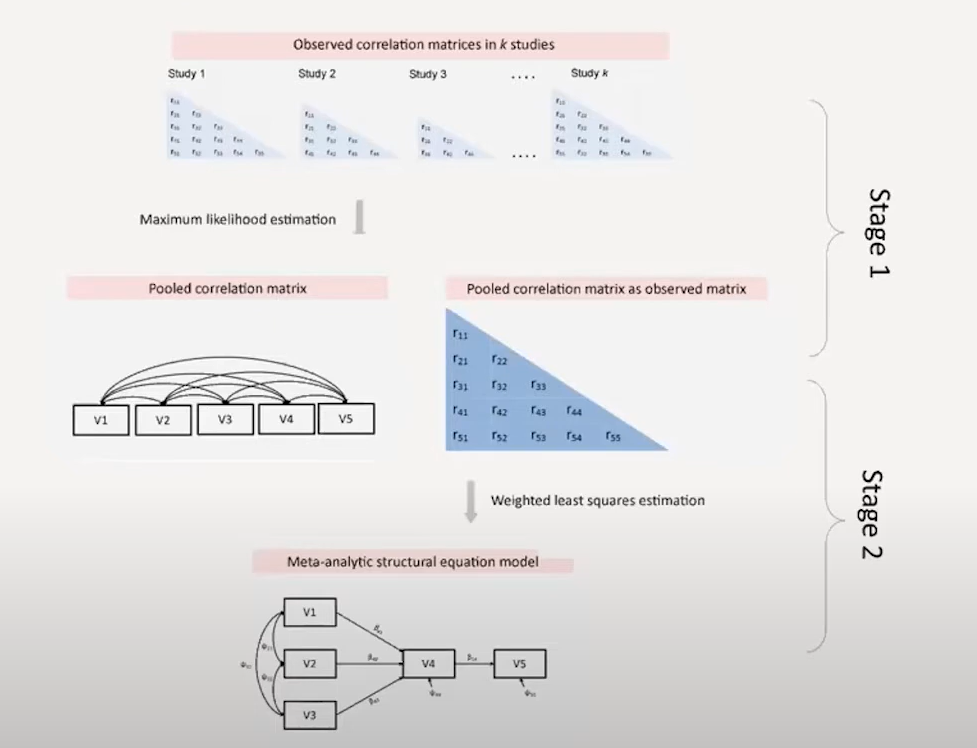
\includegraphics{images/image-230865052.png}

(image by \href{https://www.youtube.com/watch?v=0v-CdNLa_eo\&ab_channel=ZPID-LeibnizInstituteforPsychology}{Dr.~Suzanne Jak})

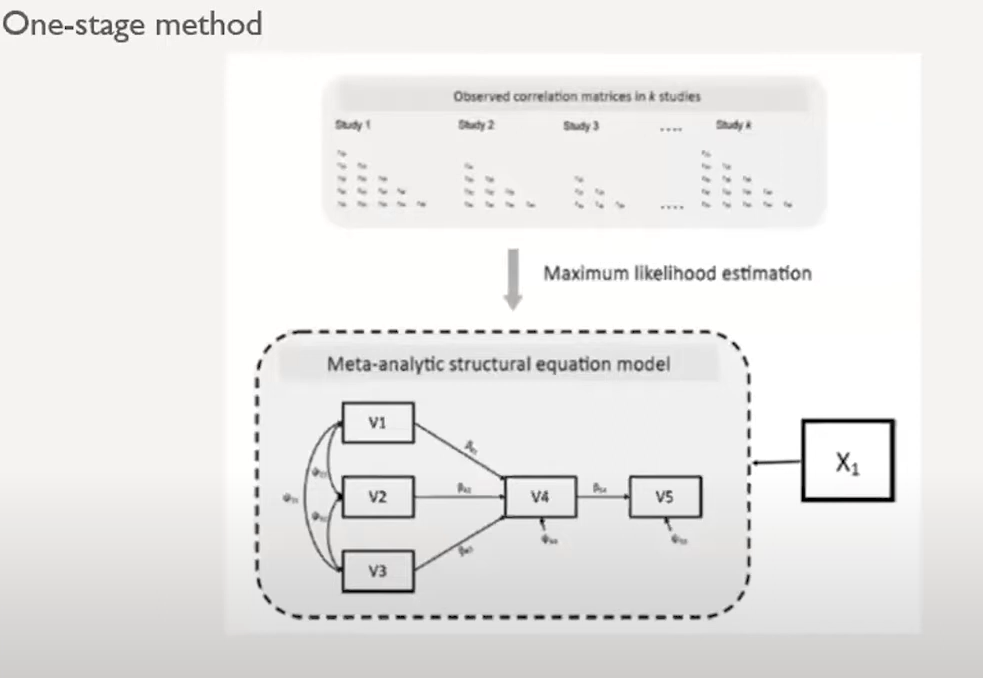
\includegraphics{images/image-105444969.png}

(image by \href{https://www.youtube.com/watch?v=0v-CdNLa_eo\&ab_channel=ZPID-LeibnizInstituteforPsychology}{Dr.~Suzanne Jak})

Steps to do MASEM \citep[p.~480]{bergh2016using}:

Step 1: Specify conceptual models:

\begin{enumerate}
\def\labelenumi{\arabic{enumi}.}
\tightlist
\item
  Specify competing models o be tested
\item
  Specify whether the models are a priori or post hoc
\end{enumerate}

Step 2: Meta-analytic procedures:

\begin{enumerate}
\def\labelenumi{\arabic{enumi}.}
\tightlist
\item
  Solutions to missing data (recommend the first three)

  \begin{enumerate}
  \def\labelenumii{\arabic{enumii}.}
  \item
    Search again (based on the same or different search criteria.
  \item
    Contact authors to request correlation values \citep{shadish1996}
  \item
    Replicate the primary study
  \item
    Use surrogate or proxy variables that are conceptually similar \citep{eby1999motivational}
  \item
    Use composite correlations by combining specific constructs into broader ones \citep{viswesvaran1995theory}
  \item
    Use a two-stage SEM \citep{cheung2005meta, fan2010factor}
  \item
    Data imputation (e.g., full information maximum likelihood) \citep{cheung2008model}
  \item
    Use the average effect size across nonmissing effect sizes \citep{viswesvaran1995theory}
  \end{enumerate}
\item
  Different pairs of variables can have different sample size values to calculate the meta-analytic correlations. Solutions:

  \begin{enumerate}
  \def\labelenumii{\arabic{enumii}.}
  \item
    Harmonic mean \citep{burke2003methodological}: \(k/(1/N_1 + 1/N_2 + \dots + 1/N_k)\) where \(k\) is the number of correlations, and \(N_k\) refers to the sample used to calculate the \(k\)-th correlation. This is \textbf{recommended} because it limits the influence of very big numbers and increases the influence of smaller values and is usually smaller than the arithmetic mean \citep{landis2013successfully, johnson2001synthetic}
  \item
    The smallest total sample size \citep{roesch2001meta}
  \item
    Median \citep{tokunaga2010evaluation}
  \item
    Arithmetic mean \citep{graham2011measuring, judge2002personality}
  \end{enumerate}
\item
  Derive meta-analytic matrix
\end{enumerate}

Step 3: Structural equation modeling

\begin{enumerate}
\def\labelenumi{\arabic{enumi}.}
\tightlist
\item
  Approaches

  \begin{enumerate}
  \def\labelenumii{\arabic{enumii}.}
  \item
    Two-stage methods \citep{cheung2005meta}

    \begin{enumerate}
    \def\labelenumiii{\arabic{enumiii}.}
    \tightlist
    \item
      can't do moderation analysis really. (can only do subgroup analysis)
    \item
      Stage 1: Combine the correlation matrices into a pooled correlation matrix
    \item
      Stage 2: Fit SEM on the pooled correlation matrix
    \item
      Can use (1) Uni variate approach \citep{hunter1990}, (2) GLM \citep{becker1992}, (3) TSSEM \citep{cheung2005meta}
    \end{enumerate}
  \item
    One-stage methods \citep{jak2020meta}

    \begin{enumerate}
    \def\labelenumiii{\arabic{enumiii}.}
    \item
      Can do moderation analysis (for continuous moderator)
    \item
      handles missing data similar to 2-stage
    \item
      provides fit indices similar to two-stage
    \item
      can use webMASEM to apply
    \end{enumerate}
  \item
    Parameter-based MASEM \citep{becker2007synthesis, gnambs2016parameter}

    \begin{enumerate}
    \def\labelenumiii{\arabic{enumiii}.}
    \item
      Steps: Fit SEM, then pool the SEM parameters
    \item
      need complete data, and model needs to fit equally well in all samples, but can be solved by Bayesian \citep{ke2019bayesian}
    \end{enumerate}
  \end{enumerate}
\item
  nonpositive definite matrix (i.e., 0 or negative eigenvalues) fix (either because of a small total number of studies in some cells, two variables are highly correlated, or overuse of imputation)

  \begin{enumerate}
  \def\labelenumii{\arabic{enumii}.}
  \item
    Choose alternative global starting values. \citep{eby1999motivational}
  \item
    Select precise starting values for parameter estimates \citep{eby1999motivational}
  \item
    Reduce the set of variables
  \end{enumerate}
\item
  Reliability missing: can either use

  \begin{enumerate}
  \def\labelenumii{\arabic{enumii}.}
  \item
    Mean reliability \citep{kirca2005market, rosengren2020meta}
  \item
    Use 0.8 as a conservative number for all constructs \citep{bergh2016using, aguinis2011debunking}
  \end{enumerate}
\item
  Sample dependencies fix:

  \begin{enumerate}
  \def\labelenumii{\arabic{enumii}.}
  \item
    \citep{geyskens2006make} recommendations in steps:

    \begin{enumerate}
    \def\labelenumiii{\arabic{enumiii}.}
    \item
      Include all meaningful correlations from each sample for consideration
    \item
      calculate composite correlation from conceptually similar component correlations from each sample
    \item
      If different studies used totally or partially overlapping datasets, choose correlation(s) based on the bigger sample size(s).
    \end{enumerate}
  \item
    use generalized least squares \citep{furlow2005meta, shadish1996}
  \item
    use random effect meta-analyses in conjunction with MASEM \citep{erez1996using}
  \item
    use multilevel meta-analytic in conjunction with MASEM \citep{van2003combining}
  \end{enumerate}
\item
  Use multiple fit measures (no general cutoff, all context-specific {[}\citet{nye2011effect})

  \begin{enumerate}
  \def\labelenumii{\arabic{enumii}.}
  \item
    Chi-square (careful because of its dependent on sample size): since MASEM can have a large number of observations, chi-square usually has poor fit even in cases where the empirical correlation matrix is quite close to the hypothesized model's correlation matrix. \citep{aguinis2009cautionary}. Hence, use other fit indices as well.

    \begin{enumerate}
    \def\labelenumiii{\arabic{enumiii}.}
    \item
      Tests the null hypothesis of exact fit
    \item
      If \(p < 0.05\), exact fit is rejected
    \end{enumerate}
  \item
    Comparative fit index (CFI)
  \item
    Goodness-of-fit index (GFI)
  \item
    Root mean square residual (RMSR): measure of approximate fit

    \begin{enumerate}
    \def\labelenumiii{\arabic{enumiii}.}
    \item
      \textless{} .05 close approximate fit
    \item
      .5 to .8 reasonable fit
    \item
      \textgreater.1 poor fit \citep{browne1992alternative}
    \end{enumerate}
  \item
    Standardized Root Mean Squared Residual (SRMSR)
  \end{enumerate}
\item
  Inclusion and exclusion criteria \citep[p.~482]{bergh2016using}:

  \begin{enumerate}
  \def\labelenumii{\arabic{enumii}.}
  \item
    Select the meta-analytic correlation for variables whose operationalizations are congruent with the a priori definitions of interest
  \item
    Select meta-analytic correlation reported by meta-analyses that used prespecified meta-analytic methodologies (e.g., how unreliability was adjusted/corrected)
  \item
    Utilize meta-analytic correlations derived from meta-analyses with the greatest sample sizes.
  \end{enumerate}
\end{enumerate}

Step 4: Reporting procedures

\begin{enumerate}
\def\labelenumi{\arabic{enumi}.}
\tightlist
\item
  Follow the meta-analysis reporting standards (MARS)

  \begin{enumerate}
  \def\labelenumii{\arabic{enumii}.}
  \tightlist
  \item
    If the model only has observed variables, the procedure should be called path analysis rather than MASEM
  \end{enumerate}
\item
  Include a table that has all estimated bivariate meta-analytic correlations and 95\% CIs for each correlation, the number of studies for each correlation (k), and the total sample size (n)
\item
  Include a table of results of each tested model with figures
\item
  Include a table of coefficients (always standardized) and statistical significance level, SEs, 95\% CIs.
\end{enumerate}

Data

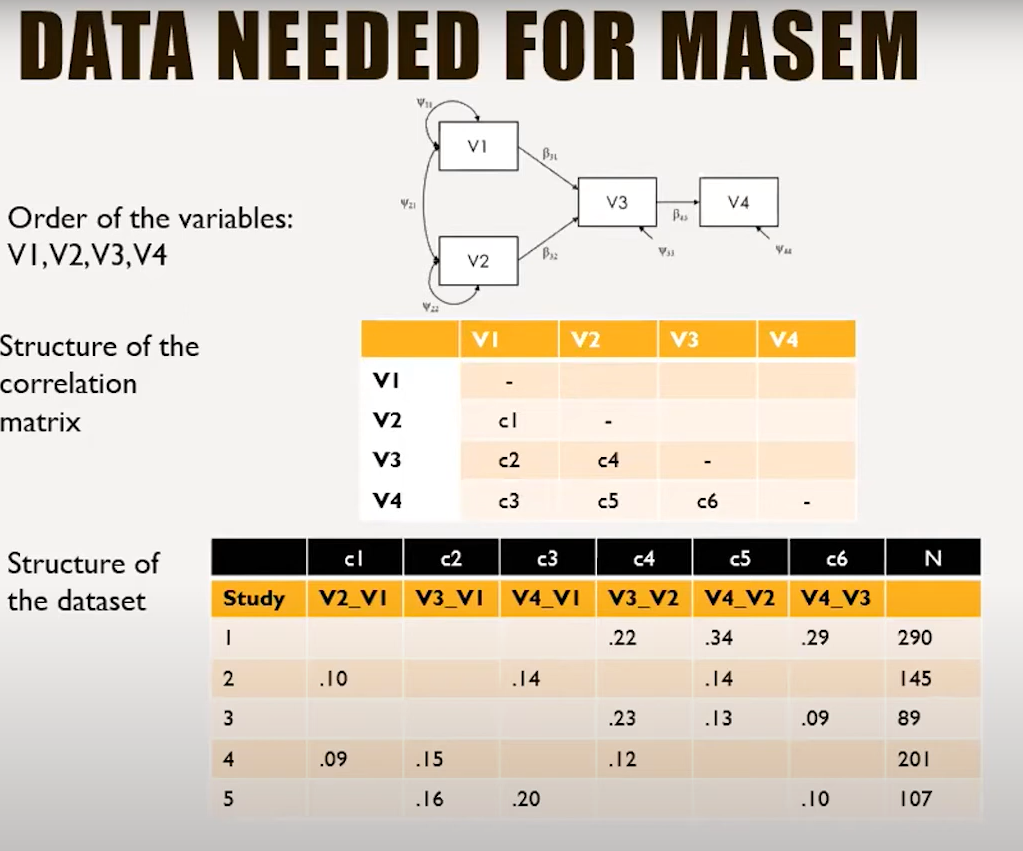
\includegraphics{images/image-325187377.png}

(image by \href{https://www.youtube.com/watch?v=0v-CdNLa_eo\&ab_channel=ZPID-LeibnizInstituteforPsychology}{Dr.~Suzanne Jak})

\hypertarget{section}{%
\section{}\label{section}}

metaSEM

\href{https://sjak.shinyapps.io/webMASEM/}{webMASEM}

\href{https://osf.io/wh6d3/}{Document}

\begin{Shaded}
\begin{Highlighting}[]
\FunctionTok{library}\NormalTok{(metaSEM)}
\FunctionTok{data}\NormalTok{(}\StringTok{"Roorda11"}\NormalTok{)}


\NormalTok{my.df }\OtherTok{\textless{}{-}} \FunctionTok{Cor2DataFrame}\NormalTok{(Roorda11}\SpecialCharTok{$}\NormalTok{data, Roorda11}\SpecialCharTok{$}\NormalTok{n)}

\DocumentationTok{\#\# Add centered SES as a moderator (standardizing SES helps to improve the stability of the results)}
\NormalTok{my.df}\SpecialCharTok{$}\NormalTok{data }\OtherTok{\textless{}{-}} \FunctionTok{data.frame}\NormalTok{(my.df}\SpecialCharTok{$}\NormalTok{data, }\AttributeTok{SES=}\FunctionTok{scale}\NormalTok{(Roorda11}\SpecialCharTok{$}\NormalTok{SES), }\AttributeTok{check.names=}\ConstantTok{FALSE}\NormalTok{)}
\FunctionTok{head}\NormalTok{(my.df}\SpecialCharTok{$}\NormalTok{data)}
\CommentTok{\#\textgreater{}   neg\_pos enga\_pos achiev\_pos enga\_neg achiev\_neg achiev\_enga}
\CommentTok{\#\textgreater{} 1   {-}0.54       NA       0.18       NA      {-}0.29          NA}
\CommentTok{\#\textgreater{} 2      NA     0.64       0.29       NA         NA        0.23}
\CommentTok{\#\textgreater{} 3      NA     0.29         NA       NA         NA          NA}
\CommentTok{\#\textgreater{} 4      NA     0.29         NA       NA         NA          NA}
\CommentTok{\#\textgreater{} 5      NA       NA         NA       NA      {-}0.24          NA}
\CommentTok{\#\textgreater{} 6      NA     0.06      {-}0.09       NA         NA        0.20}
\CommentTok{\#\textgreater{}   C(neg\_pos neg\_pos) C(enga\_pos neg\_pos) C(achiev\_pos neg\_pos)}
\CommentTok{\#\textgreater{} 1       0.0005989506       {-}0.0001515540         {-}9.072902e{-}05}
\CommentTok{\#\textgreater{} 2       0.0018375285       {-}0.0004649538         {-}2.783480e{-}04}
\CommentTok{\#\textgreater{} 3       0.0063790598       {-}0.0016141052         {-}9.662966e{-}04}
\CommentTok{\#\textgreater{} 4       0.0118882612       {-}0.0030081162         {-}1.800833e{-}03}
\CommentTok{\#\textgreater{} 5       0.0043833774       {-}0.0011091341         {-}6.639924e{-}04}
\CommentTok{\#\textgreater{} 6       0.0084368221       {-}0.0021347852         {-}1.278010e{-}03}
\CommentTok{\#\textgreater{}   C(enga\_neg neg\_pos) C(achiev\_neg neg\_pos) C(achiev\_enga neg\_pos)}
\CommentTok{\#\textgreater{} 1        0.0001507648          3.883529e{-}05          {-}2.214662e{-}05}
\CommentTok{\#\textgreater{} 2        0.0004625325          1.191427e{-}04          {-}6.794377e{-}05}
\CommentTok{\#\textgreater{} 3        0.0016057010          4.136094e{-}04          {-}2.358680e{-}04}
\CommentTok{\#\textgreater{} 4        0.0029924480          7.708155e{-}04          {-}4.395733e{-}04}
\CommentTok{\#\textgreater{} 5        0.0011033579          2.842099e{-}04          {-}1.620773e{-}04}
\CommentTok{\#\textgreater{} 6        0.0021236670          5.470291e{-}04          {-}3.119563e{-}04}
\CommentTok{\#\textgreater{}   C(enga\_pos enga\_pos) C(achiev\_pos enga\_pos) C(enga\_neg enga\_pos)}
\CommentTok{\#\textgreater{} 1         0.0006397574           0.0001647862        {-}0.0001910378}
\CommentTok{\#\textgreater{} 2         0.0019627209           0.0005055505        {-}0.0005860866}
\CommentTok{\#\textgreater{} 3         0.0068136692           0.0017550365        {-}0.0020346204}
\CommentTok{\#\textgreater{} 4         0.0126982181           0.0032707594        {-}0.0037918098}
\CommentTok{\#\textgreater{} 5         0.0046820183           0.0012059756        {-}0.0013980895}
\CommentTok{\#\textgreater{} 6         0.0090116268           0.0023211787        {-}0.0026909519}
\CommentTok{\#\textgreater{}   C(achiev\_neg enga\_pos) C(achiev\_enga enga\_pos) C(achiev\_pos achiev\_pos)}
\CommentTok{\#\textgreater{} 1          {-}5.134748e{-}05            3.127061e{-}05             0.0007526508}
\CommentTok{\#\textgreater{} 2          {-}1.575290e{-}04            9.593671e{-}05             0.0023090672}
\CommentTok{\#\textgreater{} 3          {-}5.468663e{-}04            3.330443e{-}04             0.0080160319}
\CommentTok{\#\textgreater{} 4          {-}1.019169e{-}03            6.206749e{-}04             0.0149389861}
\CommentTok{\#\textgreater{} 5          {-}3.757777e{-}04            2.288506e{-}04             0.0055082238}
\CommentTok{\#\textgreater{} 6          {-}7.232694e{-}04            4.404786e{-}04             0.0106018479}
\CommentTok{\#\textgreater{}   C(enga\_neg achiev\_pos) C(achiev\_neg achiev\_pos) C(achiev\_enga achiev\_pos)}
\CommentTok{\#\textgreater{} 1          {-}6.395603e{-}05            {-}0.0002463392              0.0001998712}
\CommentTok{\#\textgreater{} 2          {-}1.962108e{-}04            {-}0.0007557457              0.0006131884}
\CommentTok{\#\textgreater{} 3          {-}6.811498e{-}04            {-}0.0026236045              0.0021287084}
\CommentTok{\#\textgreater{} 4          {-}1.269431e{-}03            {-}0.0048894628              0.0039671437}
\CommentTok{\#\textgreater{} 5          {-}4.680533e{-}04            {-}0.0018028115              0.0014627425}
\CommentTok{\#\textgreater{} 6          {-}9.008810e{-}04            {-}0.0034699224              0.0028153850}
\CommentTok{\#\textgreater{}   C(enga\_neg enga\_neg) C(achiev\_neg enga\_neg) C(achiev\_enga enga\_neg)}
\CommentTok{\#\textgreater{} 1         0.0006389868           0.0001558889           {-}7.403068e{-}05}
\CommentTok{\#\textgreater{} 2         0.0019603566           0.0004782534           {-}2.271199e{-}04}
\CommentTok{\#\textgreater{} 3         0.0068054574           0.0016602742           {-}7.884516e{-}04}
\CommentTok{\#\textgreater{} 4         0.0126829174           0.0030941567           {-}1.469397e{-}03}
\CommentTok{\#\textgreater{} 5         0.0046763733           0.0011408577           {-}5.417848e{-}04}
\CommentTok{\#\textgreater{} 6         0.0090007701           0.0021958456           {-}1.042793e{-}03}
\CommentTok{\#\textgreater{}   C(achiev\_neg achiev\_neg) C(achiev\_enga achiev\_neg) C(achiev\_enga achiev\_enga)}
\CommentTok{\#\textgreater{} 1             0.0007298088             {-}0.0001921436               0.0006716402}
\CommentTok{\#\textgreater{} 2             0.0022389899             {-}0.0005894796               0.0020605352}
\CommentTok{\#\textgreater{} 3             0.0077727488             {-}0.0020464011               0.0071532366}
\CommentTok{\#\textgreater{} 4             0.0144856015             {-}0.0038137593               0.0133310400}
\CommentTok{\#\textgreater{} 5             0.0053410504             {-}0.0014061856               0.0049153535}
\CommentTok{\#\textgreater{} 6             0.0102800778             {-}0.0027065241               0.0094607305}
\CommentTok{\#\textgreater{}          SES}
\CommentTok{\#\textgreater{} 1  0.4464188}
\CommentTok{\#\textgreater{} 2  0.7145383}
\CommentTok{\#\textgreater{} 3  0.8821129}
\CommentTok{\#\textgreater{} 4 {-}0.8941783}
\CommentTok{\#\textgreater{} 5 {-}0.9947231}
\CommentTok{\#\textgreater{} 6 {-}0.5925439}
\end{Highlighting}
\end{Shaded}

\begin{Shaded}
\begin{Highlighting}[]
\FunctionTok{data}\NormalTok{(Scalco17)}
\NormalTok{my.df }\OtherTok{\textless{}{-}} \FunctionTok{Cor2DataFrame}\NormalTok{(Scalco17}\SpecialCharTok{$}\NormalTok{data, Scalco17}\SpecialCharTok{$}\NormalTok{n, }\AttributeTok{acov =} \StringTok{"weighted"}\NormalTok{)}

\DocumentationTok{\#\# Add the centered Age as a moderator}
\NormalTok{my.df}\SpecialCharTok{$}\NormalTok{data }\OtherTok{\textless{}{-}} \FunctionTok{data.frame}\NormalTok{(my.df}\SpecialCharTok{$}\NormalTok{data, }\AttributeTok{Age=}\FunctionTok{scale}\NormalTok{(Scalco17}\SpecialCharTok{$}\NormalTok{Age,  }\AttributeTok{scale=}\ConstantTok{FALSE}\NormalTok{), }\AttributeTok{check.names=}\ConstantTok{FALSE}\NormalTok{)}
\FunctionTok{head}\NormalTok{(my.df}\SpecialCharTok{$}\NormalTok{data)}
\CommentTok{\#\textgreater{}                                       SN\_ATT PBC\_ATT BI\_ATT BEH\_ATT PBC\_SN}
\CommentTok{\#\textgreater{} Al{-}Swidi et al., 2014                  0.562    0.18  0.798      NA  0.314}
\CommentTok{\#\textgreater{} Arvola et al., 2008 (Study A from IT)  0.690    0.44  0.730      NA  0.460}
\CommentTok{\#\textgreater{} Arvola et al., 2008 (Study A from UK)  0.520    0.22  0.600      NA  0.280}
\CommentTok{\#\textgreater{} Arvola et al., 2008 (Study A from FI)  0.570    0.40  0.670      NA  0.340}
\CommentTok{\#\textgreater{} Arvola et al., 2008 (Study B from IT)  0.760    0.35  0.710      NA  0.360}
\CommentTok{\#\textgreater{} Arvola et al., 2008 (Study B from UK)  0.460    0.03  0.550      NA  0.150}
\CommentTok{\#\textgreater{}                                       BI\_SN BEH\_SN BI\_PBC BEH\_PBC BEH\_BI}
\CommentTok{\#\textgreater{} Al{-}Swidi et al., 2014                 0.696     NA  0.216      NA     NA}
\CommentTok{\#\textgreater{} Arvola et al., 2008 (Study A from IT) 0.620     NA  0.410      NA     NA}
\CommentTok{\#\textgreater{} Arvola et al., 2008 (Study A from UK) 0.560     NA  0.310      NA     NA}
\CommentTok{\#\textgreater{} Arvola et al., 2008 (Study A from FI) 0.550     NA  0.360      NA     NA}
\CommentTok{\#\textgreater{} Arvola et al., 2008 (Study B from IT) 0.640     NA  0.240      NA     NA}
\CommentTok{\#\textgreater{} Arvola et al., 2008 (Study B from UK) 0.580     NA  0.100      NA     NA}
\CommentTok{\#\textgreater{}                                       C(SN\_ATT SN\_ATT) C(PBC\_ATT SN\_ATT)}
\CommentTok{\#\textgreater{} Al{-}Swidi et al., 2014                      0.003943225      0.0007678329}
\CommentTok{\#\textgreater{} Arvola et al., 2008 (Study A from IT)      0.003591846      0.0006994107}
\CommentTok{\#\textgreater{} Arvola et al., 2008 (Study A from UK)      0.002687225      0.0005232490}
\CommentTok{\#\textgreater{} Arvola et al., 2008 (Study A from FI)      0.003627773      0.0007064137}
\CommentTok{\#\textgreater{} Arvola et al., 2008 (Study B from IT)      0.003591851      0.0006994144}
\CommentTok{\#\textgreater{} Arvola et al., 2008 (Study B from UK)      0.002687228      0.0005232534}
\CommentTok{\#\textgreater{}                                       C(BI\_ATT SN\_ATT) C(BEH\_ATT SN\_ATT)}
\CommentTok{\#\textgreater{} Al{-}Swidi et al., 2014                     0.0011950612      0.0012021380}
\CommentTok{\#\textgreater{} Arvola et al., 2008 (Study A from IT)     0.0010885679      0.0010950127}
\CommentTok{\#\textgreater{} Arvola et al., 2008 (Study A from UK)     0.0008144034      0.0008192217}
\CommentTok{\#\textgreater{} Arvola et al., 2008 (Study A from FI)     0.0010994596      0.0011059726}
\CommentTok{\#\textgreater{} Arvola et al., 2008 (Study B from IT)     0.0010885709      0.0010950190}
\CommentTok{\#\textgreater{} Arvola et al., 2008 (Study B from UK)     0.0008144057      0.0008192250}
\CommentTok{\#\textgreater{}                                       C(PBC\_SN SN\_ATT) C(BI\_SN SN\_ATT)}
\CommentTok{\#\textgreater{} Al{-}Swidi et al., 2014                     0.0010869701     0.001853517}
\CommentTok{\#\textgreater{} Arvola et al., 2008 (Study A from IT)     0.0009901135     0.001688350}
\CommentTok{\#\textgreater{} Arvola et al., 2008 (Study A from UK)     0.0007407374     0.001263130}
\CommentTok{\#\textgreater{} Arvola et al., 2008 (Study A from FI)     0.0010000242     0.001705241}
\CommentTok{\#\textgreater{} Arvola et al., 2008 (Study B from IT)     0.0009901190     0.001688355}
\CommentTok{\#\textgreater{} Arvola et al., 2008 (Study B from UK)     0.0007407400     0.001263131}
\CommentTok{\#\textgreater{}                                       C(BEH\_SN SN\_ATT) C(BI\_PBC SN\_ATT)}
\CommentTok{\#\textgreater{} Al{-}Swidi et al., 2014                      0.001499227     0.0005441013}
\CommentTok{\#\textgreater{} Arvola et al., 2008 (Study A from IT)      0.001365631     0.0004956192}
\CommentTok{\#\textgreater{} Arvola et al., 2008 (Study A from UK)      0.001021685     0.0003707813}
\CommentTok{\#\textgreater{} Arvola et al., 2008 (Study A from FI)      0.001379297     0.0005005849}
\CommentTok{\#\textgreater{} Arvola et al., 2008 (Study B from IT)      0.001365638     0.0004956248}
\CommentTok{\#\textgreater{} Arvola et al., 2008 (Study B from UK)      0.001021687     0.0003707853}
\CommentTok{\#\textgreater{}                                       C(BEH\_PBC SN\_ATT) C(BEH\_BI SN\_ATT)}
\CommentTok{\#\textgreater{} Al{-}Swidi et al., 2014                      0.0004085977     0.0006118248}
\CommentTok{\#\textgreater{} Arvola et al., 2008 (Study A from IT)      0.0003721899     0.0005573032}
\CommentTok{\#\textgreater{} Arvola et al., 2008 (Study A from UK)      0.0002784411     0.0004169376}
\CommentTok{\#\textgreater{} Arvola et al., 2008 (Study A from FI)      0.0003759220     0.0005628839}
\CommentTok{\#\textgreater{} Arvola et al., 2008 (Study B from IT)      0.0003721961     0.0005573097}
\CommentTok{\#\textgreater{} Arvola et al., 2008 (Study B from UK)      0.0002784442     0.0004169395}
\CommentTok{\#\textgreater{}                                       C(PBC\_ATT PBC\_ATT) C(BI\_ATT PBC\_ATT)}
\CommentTok{\#\textgreater{} Al{-}Swidi et al., 2014                        0.004547982      0.0007764270}
\CommentTok{\#\textgreater{} Arvola et al., 2008 (Study A from IT)        0.004142718      0.0007072392}
\CommentTok{\#\textgreater{} Arvola et al., 2008 (Study A from UK)        0.003099353      0.0005291102}
\CommentTok{\#\textgreater{} Arvola et al., 2008 (Study A from FI)        0.004184156      0.0007143182}
\CommentTok{\#\textgreater{} Arvola et al., 2008 (Study B from IT)        0.004142722      0.0007072405}
\CommentTok{\#\textgreater{} Arvola et al., 2008 (Study B from UK)        0.003099355      0.0005291121}
\CommentTok{\#\textgreater{}                                       C(BEH\_ATT PBC\_ATT) C(PBC\_SN PBC\_ATT)}
\CommentTok{\#\textgreater{} Al{-}Swidi et al., 2014                       0.0013663069       0.001663768}
\CommentTok{\#\textgreater{} Arvola et al., 2008 (Study A from IT)       0.0012445546       0.001515516}
\CommentTok{\#\textgreater{} Arvola et al., 2008 (Study A from UK)       0.0009310978       0.001133814}
\CommentTok{\#\textgreater{} Arvola et al., 2008 (Study A from FI)       0.0012570110       0.001530681}
\CommentTok{\#\textgreater{} Arvola et al., 2008 (Study B from IT)       0.0012445593       0.001515519}
\CommentTok{\#\textgreater{} Arvola et al., 2008 (Study B from UK)       0.0009311003       0.001133816}
\CommentTok{\#\textgreater{}                                       C(BI\_SN PBC\_ATT) C(BEH\_SN PBC\_ATT)}
\CommentTok{\#\textgreater{} Al{-}Swidi et al., 2014                     0.0004362886      0.0005789500}
\CommentTok{\#\textgreater{} Arvola et al., 2008 (Study A from IT)     0.0003974112      0.0005273610}
\CommentTok{\#\textgreater{} Arvola et al., 2008 (Study A from UK)     0.0002973111      0.0003945293}
\CommentTok{\#\textgreater{} Arvola et al., 2008 (Study A from FI)     0.0004013935      0.0005326448}
\CommentTok{\#\textgreater{} Arvola et al., 2008 (Study B from IT)     0.0003974133      0.0005273648}
\CommentTok{\#\textgreater{} Arvola et al., 2008 (Study B from UK)     0.0002973136      0.0003945330}
\CommentTok{\#\textgreater{}                                       C(BI\_PBC PBC\_ATT) C(BEH\_PBC PBC\_ATT)}
\CommentTok{\#\textgreater{} Al{-}Swidi et al., 2014                       0.002592418        0.001688967}
\CommentTok{\#\textgreater{} Arvola et al., 2008 (Study A from IT)       0.002361415        0.001538469}
\CommentTok{\#\textgreater{} Arvola et al., 2008 (Study A from UK)       0.001766672        0.001150989}
\CommentTok{\#\textgreater{} Arvola et al., 2008 (Study A from FI)       0.002385040        0.001553864}
\CommentTok{\#\textgreater{} Arvola et al., 2008 (Study B from IT)       0.002361419        0.001538473}
\CommentTok{\#\textgreater{} Arvola et al., 2008 (Study B from UK)       0.001766674        0.001150991}
\CommentTok{\#\textgreater{}                                       C(BEH\_BI PBC\_ATT) C(BI\_ATT BI\_ATT)}
\CommentTok{\#\textgreater{} Al{-}Swidi et al., 2014                      0.0006653412      0.002028711}
\CommentTok{\#\textgreater{} Arvola et al., 2008 (Study A from IT)      0.0006060525      0.001847933}
\CommentTok{\#\textgreater{} Arvola et al., 2008 (Study A from UK)      0.0004534063      0.001382523}
\CommentTok{\#\textgreater{} Arvola et al., 2008 (Study A from FI)      0.0006121217      0.001866417}
\CommentTok{\#\textgreater{} Arvola et al., 2008 (Study B from IT)      0.0006060573      0.001847935}
\CommentTok{\#\textgreater{} Arvola et al., 2008 (Study B from UK)      0.0004534081      0.001382525}
\CommentTok{\#\textgreater{}                                       C(BEH\_ATT BI\_ATT) C(PBC\_SN BI\_ATT)}
\CommentTok{\#\textgreater{} Al{-}Swidi et al., 2014                      0.0012950293     0.0004215188}
\CommentTok{\#\textgreater{} Arvola et al., 2008 (Study A from IT)      0.0011796276     0.0003839583}
\CommentTok{\#\textgreater{} Arvola et al., 2008 (Study A from UK)      0.0008825291     0.0002872473}
\CommentTok{\#\textgreater{} Arvola et al., 2008 (Study A from FI)      0.0011914306     0.0003878047}
\CommentTok{\#\textgreater{} Arvola et al., 2008 (Study B from IT)      0.0011796309     0.0003839607}
\CommentTok{\#\textgreater{} Arvola et al., 2008 (Study B from UK)      0.0008825313     0.0002872486}
\CommentTok{\#\textgreater{}                                       C(BI\_SN BI\_ATT) C(BEH\_SN BI\_ATT)}
\CommentTok{\#\textgreater{} Al{-}Swidi et al., 2014                    0.0005366969     0.0005252402}
\CommentTok{\#\textgreater{} Arvola et al., 2008 (Study A from IT)    0.0004888703     0.0004784344}
\CommentTok{\#\textgreater{} Arvola et al., 2008 (Study A from UK)    0.0003657422     0.0003579326}
\CommentTok{\#\textgreater{} Arvola et al., 2008 (Study A from FI)    0.0004937645     0.0004832260}
\CommentTok{\#\textgreater{} Arvola et al., 2008 (Study B from IT)    0.0004888725     0.0004784377}
\CommentTok{\#\textgreater{} Arvola et al., 2008 (Study B from UK)    0.0003657430     0.0003579342}
\CommentTok{\#\textgreater{}                                       C(BI\_PBC BI\_ATT) C(BEH\_PBC BI\_ATT)}
\CommentTok{\#\textgreater{} Al{-}Swidi et al., 2014                     0.0005461551      0.0003593252}
\CommentTok{\#\textgreater{} Arvola et al., 2008 (Study A from IT)     0.0004974891      0.0003273071}
\CommentTok{\#\textgreater{} Arvola et al., 2008 (Study A from UK)     0.0003721847      0.0002448655}
\CommentTok{\#\textgreater{} Arvola et al., 2008 (Study A from FI)     0.0005024706      0.0003305875}
\CommentTok{\#\textgreater{} Arvola et al., 2008 (Study B from IT)     0.0004974914      0.0003273101}
\CommentTok{\#\textgreater{} Arvola et al., 2008 (Study B from UK)     0.0003721865      0.0002448671}
\CommentTok{\#\textgreater{}                                       C(BEH\_BI BI\_ATT) C(BEH\_ATT BEH\_ATT)}
\CommentTok{\#\textgreater{} Al{-}Swidi et al., 2014                     0.0005717456        0.003394130}
\CommentTok{\#\textgreater{} Arvola et al., 2008 (Study A from IT)     0.0005207960        0.003091678}
\CommentTok{\#\textgreater{} Arvola et al., 2008 (Study A from UK)     0.0003896268        0.002313023}
\CommentTok{\#\textgreater{} Arvola et al., 2008 (Study A from FI)     0.0005260094        0.003122605}
\CommentTok{\#\textgreater{} Arvola et al., 2008 (Study B from IT)     0.0005207994        0.003091684}
\CommentTok{\#\textgreater{} Arvola et al., 2008 (Study B from UK)     0.0003896281        0.002313026}
\CommentTok{\#\textgreater{}                                       C(PBC\_SN BEH\_ATT) C(BI\_SN BEH\_ATT)}
\CommentTok{\#\textgreater{} Al{-}Swidi et al., 2014                      0.0006188996     0.0006147083}
\CommentTok{\#\textgreater{} Arvola et al., 2008 (Study A from IT)      0.0005637510     0.0005599290}
\CommentTok{\#\textgreater{} Arvola et al., 2008 (Study A from UK)      0.0004217544     0.0004189019}
\CommentTok{\#\textgreater{} Arvola et al., 2008 (Study A from FI)      0.0005693995     0.0005655374}
\CommentTok{\#\textgreater{} Arvola et al., 2008 (Study B from IT)      0.0005637573     0.0005599341}
\CommentTok{\#\textgreater{} Arvola et al., 2008 (Study B from UK)      0.0004217561     0.0004189032}
\CommentTok{\#\textgreater{}                                       C(BEH\_SN BEH\_ATT) C(BI\_PBC BEH\_ATT)}
\CommentTok{\#\textgreater{} Al{-}Swidi et al., 2014                      0.0010606170      0.0007797356}
\CommentTok{\#\textgreater{} Arvola et al., 2008 (Study A from IT)      0.0009661029      0.0007102557}
\CommentTok{\#\textgreater{} Arvola et al., 2008 (Study A from UK)      0.0007227775      0.0005313609}
\CommentTok{\#\textgreater{} Arvola et al., 2008 (Study A from FI)      0.0009757752      0.0007173689}
\CommentTok{\#\textgreater{} Arvola et al., 2008 (Study B from IT)      0.0009661100      0.0007102617}
\CommentTok{\#\textgreater{} Arvola et al., 2008 (Study B from UK)      0.0007227797      0.0005313634}
\CommentTok{\#\textgreater{}                                       C(BEH\_PBC BEH\_ATT) C(BEH\_BI BEH\_ATT)}
\CommentTok{\#\textgreater{} Al{-}Swidi et al., 2014                       0.0007167328      0.0014083907}
\CommentTok{\#\textgreater{} Arvola et al., 2008 (Study A from IT)       0.0006528670      0.0012828871}
\CommentTok{\#\textgreater{} Arvola et al., 2008 (Study A from UK)       0.0004884290      0.0009597814}
\CommentTok{\#\textgreater{} Arvola et al., 2008 (Study A from FI)       0.0006594064      0.0012957243}
\CommentTok{\#\textgreater{} Arvola et al., 2008 (Study B from IT)       0.0006528733      0.0012828934}
\CommentTok{\#\textgreater{} Arvola et al., 2008 (Study B from UK)       0.0004884310      0.0009597833}
\CommentTok{\#\textgreater{}                                       C(PBC\_SN PBC\_SN) C(BI\_SN PBC\_SN)}
\CommentTok{\#\textgreater{} Al{-}Swidi et al., 2014                      0.004844329    0.0010602605}
\CommentTok{\#\textgreater{} Arvola et al., 2008 (Study A from IT)      0.004412664    0.0009657846}
\CommentTok{\#\textgreater{} Arvola et al., 2008 (Study A from UK)      0.003301311    0.0007225388}
\CommentTok{\#\textgreater{} Arvola et al., 2008 (Study A from FI)      0.004456799    0.0009754506}
\CommentTok{\#\textgreater{} Arvola et al., 2008 (Study B from IT)      0.004412667    0.0009657881}
\CommentTok{\#\textgreater{} Arvola et al., 2008 (Study B from UK)      0.003301312    0.0007225393}
\CommentTok{\#\textgreater{}                                       C(BEH\_SN PBC\_SN) C(BI\_PBC PBC\_SN)}
\CommentTok{\#\textgreater{} Al{-}Swidi et al., 2014                      0.001559436      0.002233169}
\CommentTok{\#\textgreater{} Arvola et al., 2008 (Study A from IT)      0.001420481      0.002034182}
\CommentTok{\#\textgreater{} Arvola et al., 2008 (Study A from UK)      0.001062716      0.001521853}
\CommentTok{\#\textgreater{} Arvola et al., 2008 (Study A from FI)      0.001434695      0.002054534}
\CommentTok{\#\textgreater{} Arvola et al., 2008 (Study B from IT)      0.001420486      0.002034186}
\CommentTok{\#\textgreater{} Arvola et al., 2008 (Study B from UK)      0.001062717      0.001521854}
\CommentTok{\#\textgreater{}                                       C(BEH\_PBC PBC\_SN) C(BEH\_BI PBC\_SN)}
\CommentTok{\#\textgreater{} Al{-}Swidi et al., 2014                       0.001572046     0.0006097931}
\CommentTok{\#\textgreater{} Arvola et al., 2008 (Study A from IT)       0.001431970     0.0005554571}
\CommentTok{\#\textgreater{} Arvola et al., 2008 (Study A from UK)       0.001071312     0.0004155530}
\CommentTok{\#\textgreater{} Arvola et al., 2008 (Study A from FI)       0.001446300     0.0005610200}
\CommentTok{\#\textgreater{} Arvola et al., 2008 (Study B from IT)       0.001431975     0.0005554630}
\CommentTok{\#\textgreater{} Arvola et al., 2008 (Study B from UK)       0.001071313     0.0004155533}
\CommentTok{\#\textgreater{}                                       C(BI\_SN BI\_SN) C(BEH\_SN BI\_SN)}
\CommentTok{\#\textgreater{} Al{-}Swidi et al., 2014                    0.002860047     0.001725475}
\CommentTok{\#\textgreater{} Arvola et al., 2008 (Study A from IT)    0.002605190     0.001571719}
\CommentTok{\#\textgreater{} Arvola et al., 2008 (Study A from UK)    0.001949063     0.001175872}
\CommentTok{\#\textgreater{} Arvola et al., 2008 (Study A from FI)    0.002631249     0.001587445}
\CommentTok{\#\textgreater{} Arvola et al., 2008 (Study B from IT)    0.002605194     0.001571724}
\CommentTok{\#\textgreater{} Arvola et al., 2008 (Study B from UK)    0.001949064     0.001175872}
\CommentTok{\#\textgreater{}                                       C(BI\_PBC BI\_SN) C(BEH\_PBC BI\_SN)}
\CommentTok{\#\textgreater{} Al{-}Swidi et al., 2014                    0.0005120236     0.0003559320}
\CommentTok{\#\textgreater{} Arvola et al., 2008 (Study A from IT)    0.0004664004     0.0003242175}
\CommentTok{\#\textgreater{} Arvola et al., 2008 (Study A from UK)    0.0003489245     0.0002425533}
\CommentTok{\#\textgreater{} Arvola et al., 2008 (Study A from FI)    0.0004710731     0.0003274689}
\CommentTok{\#\textgreater{} Arvola et al., 2008 (Study B from IT)    0.0004664041     0.0003242219}
\CommentTok{\#\textgreater{} Arvola et al., 2008 (Study B from UK)    0.0003489263     0.0002425544}
\CommentTok{\#\textgreater{}                                       C(BEH\_BI BI\_SN) C(BEH\_SN BEH\_SN)}
\CommentTok{\#\textgreater{} Al{-}Swidi et al., 2014                    0.0006331412      0.003763991}
\CommentTok{\#\textgreater{} Arvola et al., 2008 (Study A from IT)    0.0005767207      0.003428586}
\CommentTok{\#\textgreater{} Arvola et al., 2008 (Study A from UK)    0.0004314666      0.002565081}
\CommentTok{\#\textgreater{} Arvola et al., 2008 (Study A from FI)    0.0005824950      0.003462882}
\CommentTok{\#\textgreater{} Arvola et al., 2008 (Study B from IT)    0.0005767256      0.003428592}
\CommentTok{\#\textgreater{} Arvola et al., 2008 (Study B from UK)    0.0004314669      0.002565082}
\CommentTok{\#\textgreater{}                                       C(BI\_PBC BEH\_SN) C(BEH\_PBC BEH\_SN)}
\CommentTok{\#\textgreater{} Al{-}Swidi et al., 2014                     0.0006727061      0.0005788137}
\CommentTok{\#\textgreater{} Arvola et al., 2008 (Study A from IT)     0.0006127661      0.0005272397}
\CommentTok{\#\textgreater{} Arvola et al., 2008 (Study A from UK)     0.0004584240      0.0003944409}
\CommentTok{\#\textgreater{} Arvola et al., 2008 (Study A from FI)     0.0006189042      0.0005325228}
\CommentTok{\#\textgreater{} Arvola et al., 2008 (Study B from IT)     0.0006127711      0.0005272453}
\CommentTok{\#\textgreater{} Arvola et al., 2008 (Study B from UK)     0.0004584269      0.0003944432}
\CommentTok{\#\textgreater{}                                       C(BEH\_BI BEH\_SN) C(BI\_PBC BI\_PBC)}
\CommentTok{\#\textgreater{} Al{-}Swidi et al., 2014                     0.0011957546      0.004234763}
\CommentTok{\#\textgreater{} Arvola et al., 2008 (Study A from IT)     0.0010892004      0.003857415}
\CommentTok{\#\textgreater{} Arvola et al., 2008 (Study A from UK)     0.0008148751      0.002885902}
\CommentTok{\#\textgreater{} Arvola et al., 2008 (Study A from FI)     0.0011001009      0.003895999}
\CommentTok{\#\textgreater{} Arvola et al., 2008 (Study B from IT)     0.0010892065      0.003857419}
\CommentTok{\#\textgreater{} Arvola et al., 2008 (Study B from UK)     0.0008148760      0.002885903}
\CommentTok{\#\textgreater{}                                       C(BEH\_PBC BI\_PBC) C(BEH\_BI BI\_PBC)}
\CommentTok{\#\textgreater{} Al{-}Swidi et al., 2014                       0.002227321     0.0009451238}
\CommentTok{\#\textgreater{} Arvola et al., 2008 (Study A from IT)       0.002028854     0.0008609071}
\CommentTok{\#\textgreater{} Arvola et al., 2008 (Study A from UK)       0.001517869     0.0006440742}
\CommentTok{\#\textgreater{} Arvola et al., 2008 (Study A from FI)       0.002049152     0.0008695244}
\CommentTok{\#\textgreater{} Arvola et al., 2008 (Study B from IT)       0.002028859     0.0008609126}
\CommentTok{\#\textgreater{} Arvola et al., 2008 (Study B from UK)       0.001517871     0.0006440756}
\CommentTok{\#\textgreater{}                                       C(BEH\_PBC BEH\_PBC) C(BEH\_BI BEH\_PBC)}
\CommentTok{\#\textgreater{} Al{-}Swidi et al., 2014                        0.003778502      0.0006339252}
\CommentTok{\#\textgreater{} Arvola et al., 2008 (Study A from IT)        0.003441810      0.0005774389}
\CommentTok{\#\textgreater{} Arvola et al., 2008 (Study A from UK)        0.002574972      0.0004320001}
\CommentTok{\#\textgreater{} Arvola et al., 2008 (Study A from FI)        0.003476236      0.0005832218}
\CommentTok{\#\textgreater{} Arvola et al., 2008 (Study B from IT)        0.003441814      0.0005774445}
\CommentTok{\#\textgreater{} Arvola et al., 2008 (Study B from UK)        0.002574974      0.0004320014}
\CommentTok{\#\textgreater{}                                       C(BEH\_BI BEH\_BI)       Age}
\CommentTok{\#\textgreater{} Al{-}Swidi et al., 2014                      0.002176140 {-}2.398421}
\CommentTok{\#\textgreater{} Arvola et al., 2008 (Study A from IT)      0.001982225  2.871579}
\CommentTok{\#\textgreater{} Arvola et al., 2008 (Study A from UK)      0.001482992  2.871579}
\CommentTok{\#\textgreater{} Arvola et al., 2008 (Study A from FI)      0.002002054  2.871579}
\CommentTok{\#\textgreater{} Arvola et al., 2008 (Study B from IT)      0.001982230  2.871579}
\CommentTok{\#\textgreater{} Arvola et al., 2008 (Study B from UK)      0.001482993  2.871579}
\end{Highlighting}
\end{Shaded}

\hypertarget{univariate-approach}{%
\section{Univariate approach}\label{univariate-approach}}

\citep{viswesvaran1995}

Stage 1:

\begin{itemize}
\item
  Synthesize the correlation coefficients in a correlation matrix as if the correlation coefficients were independent
\item
  Incomplete correlation coefficients are handled by either list-wise deletion or pairwise deletion
\item
  But when using pairwise decision, missing correlations are assumed to be missing completely at random
\end{itemize}

Stage 2:

\begin{itemize}
\item
  The pooled correlation matrix is used as if it was a covariance matrix

  \begin{itemize}
  \item
    But the SEs may be incorrect
  \item
    Treating correlation matrices as covariance matrices in SEM is very dangerous \citep{cudeck1989}
  \end{itemize}
\item
  Use harmonic mean of the sample sizes as the sample size

  \begin{itemize}
  \item
    very hard to argue to have a single sample size to be used to represent the precision fo the average correlation matrix
  \item
    (some SEs can be overestimated and some can be underestimated) \citep{cudeck1989}
  \item
    Chi-square test and GOF will be affected
  \end{itemize}
\end{itemize}

\hypertarget{gls-approach}{%
\section{GLS Approach}\label{gls-approach}}

Stage 1

\begin{itemize}
\tightlist
\item
  GLS is utilized to create correlation matrices by considering the impact of sampling error.
\end{itemize}

Stage 2

\begin{itemize}
\tightlist
\item
  parameter estimates are obtained through matrix calculations and SEs are determined using the multivariate delta method.
\item
  However, this method is not easily adaptable to models that are over-identified or latent variables.
\end{itemize}

\hypertarget{tssem-approach}{%
\section{TSSEM Approach}\label{tssem-approach}}

Fixed-effects models assume that and . Random-effects models, on the other hand, treat

\hypertarget{fixed-effects}{%
\subsection{Fixed-effects}\label{fixed-effects}}

\begin{itemize}
\item
  researchers are only concerned with the specific studies included in the meta-analysis
\item
  a single correlation matrix is assumed
\item
  need to impose nonlinear constraints to ensure the diagonals are 1 \texttt{diag.constraints\ =\ T}
\end{itemize}

\hypertarget{random-effects}{%
\subsection{Random-effects}\label{random-effects}}

\begin{itemize}
\item
  the studies as samples from a larger population
\item
  researchers may want to generalize their findings to beyond the studies included in the meta-analysis
\item
  studies may have different correlation matrices
\end{itemize}

\hypertarget{application}{%
\chapter{Application}\label{application}}

Code by \href{https://osf.io/jnryt/?view_only=7eaaaedf59a8407cac5e52317b20bc3a}{Diego G Campos}

\begin{Shaded}
\begin{Highlighting}[]
\CommentTok{\# Load packages}
\FunctionTok{library}\NormalTok{(metaSEM)}
\FunctionTok{library}\NormalTok{(semPlot)}
\FunctionTok{library}\NormalTok{(lavaan)}
\FunctionTok{library}\NormalTok{(OpenMx)}
\end{Highlighting}
\end{Shaded}

\hypertarget{data-input-and-preparation}{%
\section{Data input and preparation}\label{data-input-and-preparation}}

\begin{Shaded}
\begin{Highlighting}[]
\DocumentationTok{\#\# Uncorrected correlations}
\DocumentationTok{\#\# Constructs: PU, PEU, ATT, and BI}

\CommentTok{\# Read in the correlations}
\CommentTok{\# We have 4 variables: Therefore we need 6 correlations and 4 variances}
\NormalTok{TAMu }\OtherTok{\textless{}{-}} \FunctionTok{matrix}\NormalTok{(}
    \FunctionTok{c}\NormalTok{(}\DecValTok{1}\NormalTok{,}\FloatTok{0.61}\NormalTok{,}\DecValTok{1}\NormalTok{,}\FloatTok{0.6776}\NormalTok{,}\FloatTok{0.5138}\NormalTok{,}\DecValTok{1}\NormalTok{,}\FloatTok{0.599184}\NormalTok{,}\FloatTok{0.449892}\NormalTok{,}\FloatTok{0.860328}\NormalTok{,}\DecValTok{1}\NormalTok{,}
        \DecValTok{1}\NormalTok{,}\FloatTok{0.661}\NormalTok{,}\DecValTok{1}\NormalTok{,}\FloatTok{0.59}\NormalTok{,}\FloatTok{0.584}\NormalTok{,}\DecValTok{1}\NormalTok{,}\FloatTok{0.75}\NormalTok{,}\FloatTok{0.746}\NormalTok{,}\FloatTok{0.684}\NormalTok{,}\DecValTok{1}\NormalTok{,}
        \DecValTok{1}\NormalTok{,}\FloatTok{0.5}\NormalTok{,}\DecValTok{1}\NormalTok{,}\FloatTok{0.64}\NormalTok{,}\FloatTok{0.55}\NormalTok{,}\DecValTok{1}\NormalTok{,}\FloatTok{0.55}\NormalTok{,}\FloatTok{0.48}\NormalTok{,}\FloatTok{0.59}\NormalTok{,}\DecValTok{1}\NormalTok{,}
        \DecValTok{1}\NormalTok{,}\FloatTok{0.512}\NormalTok{,}\DecValTok{1}\NormalTok{,}\FloatTok{0.461}\NormalTok{,}\FloatTok{0.754}\NormalTok{,}\DecValTok{1}\NormalTok{,}\FloatTok{0.364}\NormalTok{,}\FloatTok{0.669}\NormalTok{,}\FloatTok{0.595}\NormalTok{,}\DecValTok{1}\NormalTok{,}
        \DecValTok{1}\NormalTok{,}\FloatTok{0.279}\NormalTok{,}\DecValTok{1}\NormalTok{,}\FloatTok{0.63}\NormalTok{,}\FloatTok{0.873}\NormalTok{,}\DecValTok{1}\NormalTok{,}\FloatTok{0.319}\NormalTok{,}\FloatTok{0.441}\NormalTok{,}\FloatTok{0.505}\NormalTok{,}\DecValTok{1}\NormalTok{,}
        \DecValTok{1}\NormalTok{,}\FloatTok{0.68}\NormalTok{,}\DecValTok{1}\NormalTok{,}\FloatTok{0.68}\NormalTok{,}\FloatTok{0.73}\NormalTok{,}\DecValTok{1}\NormalTok{,}\FloatTok{0.34}\NormalTok{,}\FloatTok{0.3}\NormalTok{,}\FloatTok{0.3}\NormalTok{,}\DecValTok{1}\NormalTok{,}
        \DecValTok{1}\NormalTok{,}\FloatTok{0.4}\NormalTok{,}\DecValTok{1}\NormalTok{,}\FloatTok{0.56}\NormalTok{,}\FloatTok{0.43}\NormalTok{,}\DecValTok{1}\NormalTok{,}\FloatTok{0.23}\NormalTok{,}\FloatTok{0.32}\NormalTok{,}\FloatTok{0.36}\NormalTok{,}\DecValTok{1}\NormalTok{,}
        \DecValTok{1}\NormalTok{,}\FloatTok{0.329}\NormalTok{,}\DecValTok{1}\NormalTok{,}\FloatTok{0.565}\NormalTok{,}\FloatTok{0.349}\NormalTok{,}\DecValTok{1}\NormalTok{,}\FloatTok{0.523}\NormalTok{,}\FloatTok{0.327}\NormalTok{,}\FloatTok{0.462}\NormalTok{,}\DecValTok{1}\NormalTok{,}
        \DecValTok{1}\NormalTok{,}\FloatTok{0.136}\NormalTok{,}\DecValTok{1}\NormalTok{,}\FloatTok{0.625}\NormalTok{,}\FloatTok{0.1}\NormalTok{,}\DecValTok{1}\NormalTok{,}\FloatTok{0.436}\NormalTok{,}\FloatTok{0.1}\NormalTok{,}\FloatTok{0.514}\NormalTok{,}\DecValTok{1}\NormalTok{,}
        \DecValTok{1}\NormalTok{,}\FloatTok{0.467}\NormalTok{,}\DecValTok{1}\NormalTok{,}\FloatTok{0.634}\NormalTok{,}\FloatTok{0.61}\NormalTok{,}\DecValTok{1}\NormalTok{,}\FloatTok{0.562}\NormalTok{,}\FloatTok{0.494}\NormalTok{,}\FloatTok{0.681}\NormalTok{,}\DecValTok{1}\NormalTok{,}
        \DecValTok{1}\NormalTok{,}\FloatTok{0.62}\NormalTok{,}\DecValTok{1}\NormalTok{,}\FloatTok{0.72}\NormalTok{,}\FloatTok{0.73}\NormalTok{,}\DecValTok{1}\NormalTok{,}\FloatTok{0.76}\NormalTok{,}\FloatTok{0.6}\NormalTok{,}\FloatTok{0.71}\NormalTok{,}\DecValTok{1}\NormalTok{,}
        \DecValTok{1}\NormalTok{,}\FloatTok{0.69}\NormalTok{,}\DecValTok{1}\NormalTok{,}\FloatTok{0.76}\NormalTok{,}\FloatTok{0.71}\NormalTok{,}\DecValTok{1}\NormalTok{,}\FloatTok{0.03}\NormalTok{,}\FloatTok{0.18}\NormalTok{,}\FloatTok{0.27}\NormalTok{,}\DecValTok{1}\NormalTok{,}
        \DecValTok{1}\NormalTok{,}\FloatTok{0.067}\NormalTok{,}\DecValTok{1}\NormalTok{,}\FloatTok{0.207}\NormalTok{,}\FloatTok{0.426}\NormalTok{,}\DecValTok{1}\NormalTok{,}\FloatTok{0.199}\NormalTok{,}\FloatTok{0.076}\NormalTok{,}\FloatTok{0.006}\NormalTok{,}\DecValTok{1}\NormalTok{,}
        \DecValTok{1}\NormalTok{,}\FloatTok{0.649}\NormalTok{,}\DecValTok{1}\NormalTok{,}\FloatTok{0.525}\NormalTok{,}\FloatTok{0.408}\NormalTok{,}\DecValTok{1}\NormalTok{,}\FloatTok{0.521}\NormalTok{,}\FloatTok{0.406}\NormalTok{,}\FloatTok{0.418}\NormalTok{,}\DecValTok{1}\NormalTok{,}
        \DecValTok{1}\NormalTok{,}\FloatTok{0.3}\NormalTok{,}\DecValTok{1}\NormalTok{,}\FloatTok{0.66}\NormalTok{,}\FloatTok{0.52}\NormalTok{,}\DecValTok{1}\NormalTok{,}\FloatTok{0.57}\NormalTok{,}\FloatTok{0.26}\NormalTok{,}\FloatTok{0.5}\NormalTok{,}\DecValTok{1}\NormalTok{,}
        \DecValTok{1}\NormalTok{,}\FloatTok{0.44}\NormalTok{,}\DecValTok{1}\NormalTok{,}\FloatTok{0.62}\NormalTok{,}\FloatTok{0.51}\NormalTok{,}\DecValTok{1}\NormalTok{,}\FloatTok{0.43}\NormalTok{,}\FloatTok{0.29}\NormalTok{,}\FloatTok{0.36}\NormalTok{,}\DecValTok{1}\NormalTok{,}
        \DecValTok{1}\NormalTok{,}\FloatTok{0.449}\NormalTok{,}\DecValTok{1}\NormalTok{,}\FloatTok{0.791}\NormalTok{,}\FloatTok{0.509}\NormalTok{,}\DecValTok{1}\NormalTok{,}\FloatTok{0.362}\NormalTok{,}\FloatTok{0.217}\NormalTok{,}\FloatTok{0.412}\NormalTok{,}\DecValTok{1}\NormalTok{,}
        \DecValTok{1}\NormalTok{,}\FloatTok{0.392}\NormalTok{,}\DecValTok{1}\NormalTok{,}\FloatTok{0.682}\NormalTok{,}\FloatTok{0.446}\NormalTok{,}\DecValTok{1}\NormalTok{,}\FloatTok{0.327}\NormalTok{,}\FloatTok{0.188}\NormalTok{,}\FloatTok{0.442}\NormalTok{,}\DecValTok{1}\NormalTok{,}
        \DecValTok{1}\NormalTok{,}\FloatTok{0.11}\NormalTok{,}\DecValTok{1}\NormalTok{,}\FloatTok{0.75}\NormalTok{,}\FloatTok{0.11}\NormalTok{,}\DecValTok{1}\NormalTok{,}\FloatTok{0.62}\NormalTok{,}\FloatTok{0.2}\NormalTok{,}\FloatTok{0.67}\NormalTok{,}\DecValTok{1}\NormalTok{,}
        \DecValTok{1}\NormalTok{,}\FloatTok{0.41}\NormalTok{,}\DecValTok{1}\NormalTok{,}\FloatTok{0.54}\NormalTok{,}\FloatTok{0.51}\NormalTok{,}\DecValTok{1}\NormalTok{,}\FloatTok{0.4}\NormalTok{,}\FloatTok{0.43}\NormalTok{,}\FloatTok{0.54}\NormalTok{,}\DecValTok{1}\NormalTok{,}
        \DecValTok{1}\NormalTok{,}\FloatTok{0.656}\NormalTok{,}\DecValTok{1}\NormalTok{,}\FloatTok{0.8358}\NormalTok{,}\FloatTok{0.564}\NormalTok{,}\DecValTok{1}\NormalTok{,}\FloatTok{0.643}\NormalTok{,}\FloatTok{0.5431}\NormalTok{,}\FloatTok{0.5299}\NormalTok{,}\DecValTok{1}\NormalTok{,}
        \DecValTok{1}\NormalTok{,}\FloatTok{0.33}\NormalTok{,}\DecValTok{1}\NormalTok{,}\FloatTok{0.63}\NormalTok{,}\FloatTok{0.5}\NormalTok{,}\DecValTok{1}\NormalTok{,}\FloatTok{0.738}\NormalTok{,}\FloatTok{0.311}\NormalTok{,}\FloatTok{0.527}\NormalTok{,}\DecValTok{1}\NormalTok{,}
        \DecValTok{1}\NormalTok{,}\FloatTok{0.23}\NormalTok{,}\DecValTok{1}\NormalTok{,}\FloatTok{0.46}\NormalTok{,}\FloatTok{0.35}\NormalTok{,}\DecValTok{1}\NormalTok{,}\FloatTok{0.43}\NormalTok{,}\FloatTok{0.19}\NormalTok{,}\FloatTok{0.44}\NormalTok{,}\DecValTok{1}\NormalTok{,}
        \DecValTok{1}\NormalTok{,}\FloatTok{0.44}\NormalTok{,}\DecValTok{1}\NormalTok{,}\FloatTok{0.61}\NormalTok{,}\FloatTok{0.48}\NormalTok{,}\DecValTok{1}\NormalTok{,}\FloatTok{0.68}\NormalTok{,}\FloatTok{0.33}\NormalTok{,}\FloatTok{0.55}\NormalTok{,}\DecValTok{1}\NormalTok{,}
        \DecValTok{1}\NormalTok{,}\FloatTok{0.72}\NormalTok{,}\DecValTok{1}\NormalTok{,}\FloatTok{0.71}\NormalTok{,}\FloatTok{0.7}\NormalTok{,}\DecValTok{1}\NormalTok{,}\FloatTok{0.73}\NormalTok{,}\FloatTok{0.65}\NormalTok{,}\FloatTok{0.68}\NormalTok{,}\DecValTok{1}\NormalTok{,}
        \DecValTok{1}\NormalTok{,}\FloatTok{0.52}\NormalTok{,}\DecValTok{1}\NormalTok{,}\FloatTok{0.535}\NormalTok{,}\FloatTok{0.51}\NormalTok{,}\DecValTok{1}\NormalTok{,}\FloatTok{0.707}\NormalTok{,}\FloatTok{0.553}\NormalTok{,}\FloatTok{0.437}\NormalTok{,}\DecValTok{1}\NormalTok{,}
        \DecValTok{1}\NormalTok{,}\FloatTok{0.54}\NormalTok{,}\DecValTok{1}\NormalTok{,}\FloatTok{0.64}\NormalTok{,}\FloatTok{0.56}\NormalTok{,}\DecValTok{1}\NormalTok{,}\FloatTok{0.54}\NormalTok{,}\FloatTok{0.38}\NormalTok{,}\FloatTok{0.61}\NormalTok{,}\DecValTok{1}\NormalTok{,}
        \DecValTok{1}\NormalTok{,}\FloatTok{0.53}\NormalTok{,}\DecValTok{1}\NormalTok{,}\FloatTok{0.63}\NormalTok{,}\FloatTok{0.65}\NormalTok{,}\DecValTok{1}\NormalTok{,}\FloatTok{0.57}\NormalTok{,}\FloatTok{0.51}\NormalTok{,}\FloatTok{0.69}\NormalTok{,}\DecValTok{1}\NormalTok{,}
        \DecValTok{1}\NormalTok{,}\FloatTok{0.54}\NormalTok{,}\DecValTok{1}\NormalTok{,}\FloatTok{0.46}\NormalTok{,}\FloatTok{0.44}\NormalTok{,}\DecValTok{1}\NormalTok{,}\FloatTok{0.35}\NormalTok{,}\FloatTok{0.22}\NormalTok{,}\FloatTok{0.21}\NormalTok{,}\DecValTok{1}\NormalTok{,}
        \DecValTok{1}\NormalTok{,}\FloatTok{0.36}\NormalTok{,}\DecValTok{1}\NormalTok{,}\FloatTok{0.57}\NormalTok{,}\FloatTok{0.48}\NormalTok{,}\DecValTok{1}\NormalTok{,}\FloatTok{0.16}\NormalTok{,}\FloatTok{0.17}\NormalTok{,}\FloatTok{0.13}\NormalTok{,}\DecValTok{1}\NormalTok{,}
        \DecValTok{1}\NormalTok{,}\FloatTok{0.44}\NormalTok{,}\DecValTok{1}\NormalTok{,}\FloatTok{0.63}\NormalTok{,}\FloatTok{0.47}\NormalTok{,}\DecValTok{1}\NormalTok{,}\FloatTok{0.63}\NormalTok{,}\FloatTok{0.41}\NormalTok{,}\FloatTok{0.62}\NormalTok{,}\DecValTok{1}\NormalTok{,}
        \DecValTok{1}\NormalTok{,}\FloatTok{0.44}\NormalTok{,}\DecValTok{1}\NormalTok{,}\FloatTok{0.61}\NormalTok{,}\FloatTok{0.49}\NormalTok{,}\DecValTok{1}\NormalTok{,}\FloatTok{0.41}\NormalTok{,}\FloatTok{0.3}\NormalTok{,}\FloatTok{0.4}\NormalTok{,}\DecValTok{1}\NormalTok{,}
        \DecValTok{1}\NormalTok{,}\FloatTok{0.66}\NormalTok{,}\DecValTok{1}\NormalTok{,}\FloatTok{0.28}\NormalTok{,}\FloatTok{0.2}\NormalTok{,}\DecValTok{1}\NormalTok{,}\FloatTok{0.58}\NormalTok{,}\FloatTok{0.5}\NormalTok{,}\FloatTok{0.07}\NormalTok{,}\DecValTok{1}\NormalTok{,}
        \DecValTok{1}\NormalTok{,}\FloatTok{0.53}\NormalTok{,}\DecValTok{1}\NormalTok{,}\FloatTok{0.81}\NormalTok{,}\FloatTok{0.67}\NormalTok{,}\DecValTok{1}\NormalTok{,}\FloatTok{0.7}\NormalTok{,}\FloatTok{0.63}\NormalTok{,}\FloatTok{0.69}\NormalTok{,}\DecValTok{1}\NormalTok{,}
        \DecValTok{1}\NormalTok{,}\FloatTok{0.61}\NormalTok{,}\DecValTok{1}\NormalTok{,}\FloatTok{0.6}\NormalTok{,}\FloatTok{0.64}\NormalTok{,}\DecValTok{1}\NormalTok{,}\FloatTok{0.62}\NormalTok{,}\FloatTok{0.59}\NormalTok{,}\FloatTok{0.71}\NormalTok{,}\DecValTok{1}\NormalTok{,}
        \DecValTok{1}\NormalTok{,}\FloatTok{0.62}\NormalTok{,}\DecValTok{1}\NormalTok{,}\FloatTok{0.71}\NormalTok{,}\FloatTok{0.55}\NormalTok{,}\DecValTok{1}\NormalTok{,}\FloatTok{0.66}\NormalTok{,}\FloatTok{0.56}\NormalTok{,}\FloatTok{0.84}\NormalTok{,}\DecValTok{1}\NormalTok{,}
        \DecValTok{1}\NormalTok{,}\FloatTok{0.575}\NormalTok{,}\DecValTok{1}\NormalTok{,}\FloatTok{0.486}\NormalTok{,}\FloatTok{0.453}\NormalTok{,}\DecValTok{1}\NormalTok{,}\FloatTok{0.351}\NormalTok{,}\FloatTok{0.297}\NormalTok{,}\FloatTok{0.447}\NormalTok{,}\DecValTok{1}\NormalTok{,}
        \DecValTok{1}\NormalTok{,}\FloatTok{0.749}\NormalTok{,}\DecValTok{1}\NormalTok{,}\FloatTok{0.508}\NormalTok{,}\FloatTok{0.258}\NormalTok{,}\DecValTok{1}\NormalTok{,}\FloatTok{0.872}\NormalTok{,}\FloatTok{0.743}\NormalTok{,}\FloatTok{0.461}\NormalTok{,}\DecValTok{1}\NormalTok{,}
        \DecValTok{1}\NormalTok{,}\FloatTok{0.61}\NormalTok{,}\DecValTok{1}\NormalTok{,}\FloatTok{0.63}\NormalTok{,}\FloatTok{0.67}\NormalTok{,}\DecValTok{1}\NormalTok{,}\FloatTok{0.64}\NormalTok{,}\FloatTok{0.59}\NormalTok{,}\FloatTok{0.75}\NormalTok{,}\DecValTok{1}\NormalTok{,}
        \DecValTok{1}\NormalTok{,}\FloatTok{0.31}\NormalTok{,}\DecValTok{1}\NormalTok{,}\FloatTok{0.23}\NormalTok{,}\FloatTok{0.61}\NormalTok{,}\DecValTok{1}\NormalTok{,}\FloatTok{0.28}\NormalTok{,}\FloatTok{0.53}\NormalTok{,}\FloatTok{0.53}\NormalTok{,}\DecValTok{1}\NormalTok{,}
        \DecValTok{1}\NormalTok{,}\FloatTok{0.65}\NormalTok{,}\DecValTok{1}\NormalTok{,}\FloatTok{0.51}\NormalTok{,}\FloatTok{0.35}\NormalTok{,}\DecValTok{1}\NormalTok{,}\FloatTok{0.5}\NormalTok{,}\FloatTok{0.41}\NormalTok{,}\FloatTok{0.42}\NormalTok{,}\DecValTok{1}\NormalTok{,}
        \DecValTok{1}\NormalTok{,}\FloatTok{0.526}\NormalTok{,}\DecValTok{1}\NormalTok{,}\FloatTok{0.681}\NormalTok{,}\FloatTok{0.585}\NormalTok{,}\DecValTok{1}\NormalTok{,}\FloatTok{0.654}\NormalTok{,}\FloatTok{0.445}\NormalTok{,}\FloatTok{0.684}\NormalTok{,}\DecValTok{1}\NormalTok{,}
        \DecValTok{1}\NormalTok{,}\FloatTok{0.307}\NormalTok{,}\DecValTok{1}\NormalTok{,}\FloatTok{0.632}\NormalTok{,}\FloatTok{0.462}\NormalTok{,}\DecValTok{1}\NormalTok{,}\FloatTok{0.586}\NormalTok{,}\FloatTok{0.283}\NormalTok{,}\FloatTok{0.446}\NormalTok{,}\DecValTok{1}\NormalTok{,}
        \DecValTok{1}\NormalTok{,}\FloatTok{0.517}\NormalTok{,}\DecValTok{1}\NormalTok{,}\FloatTok{0.6}\NormalTok{,}\FloatTok{0.527}\NormalTok{,}\DecValTok{1}\NormalTok{,}\FloatTok{0.548}\NormalTok{,}\FloatTok{0.405}\NormalTok{,}\FloatTok{0.687}\NormalTok{,}\DecValTok{1}\NormalTok{,}
        \DecValTok{1}\NormalTok{,}\FloatTok{0.64}\NormalTok{,}\DecValTok{1}\NormalTok{,}\FloatTok{0.65}\NormalTok{,}\FloatTok{0.65}\NormalTok{,}\DecValTok{1}\NormalTok{,}\FloatTok{0.61}\NormalTok{,}\FloatTok{0.65}\NormalTok{,}\FloatTok{0.75}\NormalTok{,}\DecValTok{1}\NormalTok{,}
        \DecValTok{1}\NormalTok{,}\FloatTok{0.26}\NormalTok{,}\DecValTok{1}\NormalTok{,}\FloatTok{0.549}\NormalTok{,}\FloatTok{0.497}\NormalTok{,}\DecValTok{1}\NormalTok{,}\FloatTok{0.192}\NormalTok{,}\FloatTok{0.265}\NormalTok{,}\FloatTok{0.249}\NormalTok{,}\DecValTok{1}\NormalTok{,}
        \DecValTok{1}\NormalTok{,}\FloatTok{0.26}\NormalTok{,}\DecValTok{1}\NormalTok{,}\FloatTok{0.551}\NormalTok{,}\FloatTok{0.507}\NormalTok{,}\DecValTok{1}\NormalTok{,}\FloatTok{0.176}\NormalTok{,}\FloatTok{0.101}\NormalTok{,}\FloatTok{0.257}\NormalTok{,}\DecValTok{1}\NormalTok{,}
        \DecValTok{1}\NormalTok{,}\FloatTok{0.5376}\NormalTok{,}\DecValTok{1}\NormalTok{,}\FloatTok{0.6336}\NormalTok{,}\FloatTok{0.8396}\NormalTok{,}\DecValTok{1}\NormalTok{,}\FloatTok{0.8905}\NormalTok{,}\FloatTok{0.6887}\NormalTok{,}\FloatTok{0.8154}\NormalTok{,}\DecValTok{1}\NormalTok{,}
        \DecValTok{1}\NormalTok{,}\FloatTok{0.709}\NormalTok{,}\DecValTok{1}\NormalTok{,}\FloatTok{0.885}\NormalTok{,}\FloatTok{0.768}\NormalTok{,}\DecValTok{1}\NormalTok{,}\FloatTok{0.758}\NormalTok{,}\FloatTok{0.589}\NormalTok{,}\FloatTok{0.783}\NormalTok{,}\DecValTok{1}\NormalTok{,}
        \DecValTok{1}\NormalTok{,}\FloatTok{0.49}\NormalTok{,}\DecValTok{1}\NormalTok{,}\FloatTok{0.63}\NormalTok{,}\FloatTok{0.53}\NormalTok{,}\DecValTok{1}\NormalTok{,}\FloatTok{0.63}\NormalTok{,}\FloatTok{0.46}\NormalTok{,}\FloatTok{0.62}\NormalTok{,}\DecValTok{1}\NormalTok{),}
    \AttributeTok{ncol=}\DecValTok{10}\NormalTok{, }\AttributeTok{byrow=}\ConstantTok{TRUE}\NormalTok{)    }\CommentTok{\# fill in correlations row by row with the variances}

\CommentTok{\# Split the above{-}created matrix into matrices for single studies}
\CommentTok{\# 50 studies in total}
\CommentTok{\# 4x4 correlation matrices}
\NormalTok{TAMu }\OtherTok{\textless{}{-}} \FunctionTok{lapply}\NormalTok{(}\FunctionTok{split}\NormalTok{(TAMu, }\DecValTok{1}\SpecialCharTok{:}\DecValTok{50}\NormalTok{), }\CommentTok{\# split rows into separate studies}
                                  \CommentTok{\# 50 studies }
                   \ControlFlowTok{function}\NormalTok{(x) \{mat }\OtherTok{\textless{}{-}} \FunctionTok{matrix}\NormalTok{(}\DecValTok{1}\NormalTok{, }\AttributeTok{ncol=}\DecValTok{4}\NormalTok{, }\AttributeTok{nrow=}\DecValTok{4}\NormalTok{);   }\CommentTok{\# create matrix with 1\textquotesingle{}s}
\NormalTok{                   mat[}\FunctionTok{upper.tri}\NormalTok{(mat, }\AttributeTok{diag=}\ConstantTok{TRUE}\NormalTok{)] }\OtherTok{\textless{}{-}}\NormalTok{ x;     }\CommentTok{\# fill upper matrix and diagonals}
\NormalTok{                   mat[}\FunctionTok{lower.tri}\NormalTok{(mat)] }\OtherTok{\textless{}{-}} \FunctionTok{t}\NormalTok{(mat)[}\FunctionTok{lower.tri}\NormalTok{(mat)];   }\CommentTok{\# fill lower matrix}
\NormalTok{                   mat\})}

\CommentTok{\# Name variables}
\NormalTok{TAMu }\OtherTok{\textless{}{-}} \FunctionTok{lapply}\NormalTok{(TAMu, }\ControlFlowTok{function}\NormalTok{(x, var.names) \{}\FunctionTok{dimnames}\NormalTok{(x) }\OtherTok{\textless{}{-}} \FunctionTok{list}\NormalTok{(var.names, var.names); x\},}
                   \AttributeTok{var.names=}\FunctionTok{c}\NormalTok{(}\StringTok{"PU"}\NormalTok{, }\StringTok{"PEU"}\NormalTok{, }\StringTok{"ATT"}\NormalTok{, }\StringTok{"BI"}\NormalTok{))   }\CommentTok{\# create variable names                }

\CommentTok{\# Study names}
\FunctionTok{names}\NormalTok{(TAMu) }\OtherTok{\textless{}{-}} \FunctionTok{c}\NormalTok{(}\StringTok{"Okazaki \& Renda dos Santos (2012)"}\NormalTok{,}
                    \StringTok{"Parkman (2015)"}\NormalTok{,}
                    \StringTok{"Wong (2015)"}\NormalTok{,}
                    \StringTok{"Cote \& Miliner (2015)"}\NormalTok{,}
                    \StringTok{"Teo \& Milutinovic (2015)"}\NormalTok{,}
                    \StringTok{"Teo \& Fan et al. (2015){-}1"}\NormalTok{,}
                    \StringTok{"Teo \& Fan et al. (2015){-}2"}\NormalTok{,}
                    \StringTok{"Koutromanos et al. (2015){-}1"}\NormalTok{,}
                    \StringTok{"Koutromanos et al. (2015){-}2"}\NormalTok{,}
                    \StringTok{"Wu et al. (2015)"}\NormalTok{,}
                    \StringTok{"Kabakci{-}Yurdakul et al. (2014)"}\NormalTok{,}
                    \StringTok{"Kirmizi (2014)"}\NormalTok{,}
                    \StringTok{"Mac Callum et al. (2014)"}\NormalTok{,}
                    \StringTok{"Wong et al. (2013)"}\NormalTok{,}
                    \StringTok{"Teo \& Ursavas et al. (2011a)"}\NormalTok{,}
                    \StringTok{"Teo \& Luan et al. (2008)"}\NormalTok{,}
                    \StringTok{"Sumak \& Sorgo (2016){-}1"}\NormalTok{,}
                    \StringTok{"Sumak \& Sorgo (2016){-}2"}\NormalTok{,}
                    \StringTok{"Wu et al. (2016)"}\NormalTok{,}
                    \StringTok{"Wong et al. (2016)"}\NormalTok{,}
                    \StringTok{"Atif et al. (2015)"}\NormalTok{,}
                    \StringTok{"Tokel \& Isler (2015)"}\NormalTok{,}
                    \StringTok{"Sadeghi et al. (2014)"}\NormalTok{,}
                    \StringTok{"Pynoo et al. (2012)"}\NormalTok{,}
                    \StringTok{"Aypay et al. (2012)"}\NormalTok{,}
                    \StringTok{"Chen \& Tseng (2012)"}\NormalTok{,}
                    \StringTok{"Teo (2012a)"}\NormalTok{,}
                    \StringTok{"Teo \& van Schaik (2012)"}\NormalTok{,}
                    \StringTok{"Teo \& Noyes (2011)"}\NormalTok{,}
                    \StringTok{"Teo \& Lee et al. (2009a){-}1"}\NormalTok{,}
                    \StringTok{"Teo \& Lee et al. (2009a){-}2"}\NormalTok{,}
                    \StringTok{"Teo (2009a)"}\NormalTok{,}
                    \StringTok{"Park et al. (2007)"}\NormalTok{,}
                    \StringTok{"Cheung \& Sachs (2006)"}\NormalTok{,}
                    \StringTok{"Teo (2011)"}\NormalTok{,}
                    \StringTok{"Shiue (2007)"}\NormalTok{,}
                    \StringTok{"Chiu (2017)"}\NormalTok{,}
                    \StringTok{"Lai et al. (2013)"}\NormalTok{,}
                    \StringTok{"Teo \& Zhou et al. (2016)"}\NormalTok{,}
                    \StringTok{"Teo (2008)"}\NormalTok{,}
                    \StringTok{"Wong \& Teo et al. (2012)"}\NormalTok{,}
                    \StringTok{"Luan \& Teo (2009)"}\NormalTok{,}
                    \StringTok{"Teo \& Ursavas et al. (2012)"}\NormalTok{,}
                    \StringTok{"Teo \& Zhou (2014)"}\NormalTok{,}
                    \StringTok{"Teo (2013)"}\NormalTok{,}
                    \StringTok{"Teo \& Milutinovic et al. (2016a){-}1"}\NormalTok{,}
                    \StringTok{"Teo \& Milutinovic et al. (2016a){-}2"}\NormalTok{,}
                    \StringTok{"Pittalis \& Christou (2010)"}\NormalTok{,}
                    \StringTok{"Fathema et al. (2015)"}\NormalTok{,}
                    \StringTok{"Luan \& Teo (2011)"}\NormalTok{)}

\CommentTok{\# Sample sizes}
\NormalTok{TAM.n }\OtherTok{\textless{}{-}} \FunctionTok{c}\NormalTok{(}\DecValTok{446}\NormalTok{,}\DecValTok{88}\NormalTok{,}\DecValTok{234}\NormalTok{,}\DecValTok{29}\NormalTok{,}\DecValTok{313}\NormalTok{,}\DecValTok{169}\NormalTok{,}\DecValTok{170}\NormalTok{,}\DecValTok{151}\NormalTok{,}\DecValTok{106}\NormalTok{,}\DecValTok{340}\NormalTok{,}\DecValTok{579}\NormalTok{,}
            \DecValTok{213}\NormalTok{,}\DecValTok{196}\NormalTok{,}\DecValTok{302}\NormalTok{,}\DecValTok{197}\NormalTok{,}\DecValTok{495}\NormalTok{,}\DecValTok{438}\NormalTok{,}\DecValTok{460}\NormalTok{,}\DecValTok{144}\NormalTok{,}\DecValTok{185}\NormalTok{,}\DecValTok{184}\NormalTok{,}\DecValTok{46}\NormalTok{,}\DecValTok{275}\NormalTok{,}
            \DecValTok{919}\NormalTok{,}\DecValTok{754}\NormalTok{,}\DecValTok{402}\NormalTok{,}\DecValTok{157}\NormalTok{,}\DecValTok{429}\NormalTok{,}\DecValTok{153}\NormalTok{,}\DecValTok{250}\NormalTok{,}\DecValTok{245}\NormalTok{,}\DecValTok{475}\NormalTok{,}\DecValTok{191}\NormalTok{,}\DecValTok{57}\NormalTok{,}\DecValTok{592}\NormalTok{,}
            \DecValTok{242}\NormalTok{,}\DecValTok{306}\NormalTok{,}\DecValTok{160}\NormalTok{,}\DecValTok{592}\NormalTok{,}\DecValTok{139}\NormalTok{,}\DecValTok{302}\NormalTok{,}\DecValTok{245}\NormalTok{,}\DecValTok{487}\NormalTok{,}\DecValTok{314}\NormalTok{,}\DecValTok{385}\NormalTok{,}\DecValTok{226}\NormalTok{,}
            \DecValTok{226}\NormalTok{,}\DecValTok{105}\NormalTok{,}\DecValTok{560}\NormalTok{,}\DecValTok{245}\NormalTok{)}

\DocumentationTok{\#\#\#\#\#\#\#\#\#\#\#\#\#\#\#\#\#   }
\CommentTok{\# Combine everything in an object}
\NormalTok{TAMu }\OtherTok{\textless{}{-}} \FunctionTok{list}\NormalTok{(}\AttributeTok{data=}\NormalTok{TAMu, }\AttributeTok{n=}\NormalTok{TAM.n)}
\FunctionTok{head}\NormalTok{(TAMu}\SpecialCharTok{$}\NormalTok{data)}
\CommentTok{\#\textgreater{} $\textasciigrave{}Okazaki \& Renda dos Santos (2012)\textasciigrave{}}
\CommentTok{\#\textgreater{}           PU      PEU      ATT       BI}
\CommentTok{\#\textgreater{} PU  1.000000 0.610000 0.677600 0.599184}
\CommentTok{\#\textgreater{} PEU 0.610000 1.000000 0.513800 0.449892}
\CommentTok{\#\textgreater{} ATT 0.677600 0.513800 1.000000 0.860328}
\CommentTok{\#\textgreater{} BI  0.599184 0.449892 0.860328 1.000000}
\CommentTok{\#\textgreater{} }
\CommentTok{\#\textgreater{} $\textasciigrave{}Parkman (2015)\textasciigrave{}}
\CommentTok{\#\textgreater{}        PU   PEU   ATT    BI}
\CommentTok{\#\textgreater{} PU  1.000 0.661 0.590 0.750}
\CommentTok{\#\textgreater{} PEU 0.661 1.000 0.584 0.746}
\CommentTok{\#\textgreater{} ATT 0.590 0.584 1.000 0.684}
\CommentTok{\#\textgreater{} BI  0.750 0.746 0.684 1.000}
\CommentTok{\#\textgreater{} }
\CommentTok{\#\textgreater{} $\textasciigrave{}Wong (2015)\textasciigrave{}}
\CommentTok{\#\textgreater{}       PU  PEU  ATT   BI}
\CommentTok{\#\textgreater{} PU  1.00 0.50 0.64 0.55}
\CommentTok{\#\textgreater{} PEU 0.50 1.00 0.55 0.48}
\CommentTok{\#\textgreater{} ATT 0.64 0.55 1.00 0.59}
\CommentTok{\#\textgreater{} BI  0.55 0.48 0.59 1.00}
\CommentTok{\#\textgreater{} }
\CommentTok{\#\textgreater{} $\textasciigrave{}Cote \& Miliner (2015)\textasciigrave{}}
\CommentTok{\#\textgreater{}        PU   PEU   ATT    BI}
\CommentTok{\#\textgreater{} PU  1.000 0.512 0.461 0.364}
\CommentTok{\#\textgreater{} PEU 0.512 1.000 0.754 0.669}
\CommentTok{\#\textgreater{} ATT 0.461 0.754 1.000 0.595}
\CommentTok{\#\textgreater{} BI  0.364 0.669 0.595 1.000}
\CommentTok{\#\textgreater{} }
\CommentTok{\#\textgreater{} $\textasciigrave{}Teo \& Milutinovic (2015)\textasciigrave{}}
\CommentTok{\#\textgreater{}        PU   PEU   ATT    BI}
\CommentTok{\#\textgreater{} PU  1.000 0.279 0.630 0.319}
\CommentTok{\#\textgreater{} PEU 0.279 1.000 0.873 0.441}
\CommentTok{\#\textgreater{} ATT 0.630 0.873 1.000 0.505}
\CommentTok{\#\textgreater{} BI  0.319 0.441 0.505 1.000}
\CommentTok{\#\textgreater{} }
\CommentTok{\#\textgreater{} $\textasciigrave{}Teo \& Fan et al. (2015){-}1\textasciigrave{}}
\CommentTok{\#\textgreater{}       PU  PEU  ATT   BI}
\CommentTok{\#\textgreater{} PU  1.00 0.68 0.68 0.34}
\CommentTok{\#\textgreater{} PEU 0.68 1.00 0.73 0.30}
\CommentTok{\#\textgreater{} ATT 0.68 0.73 1.00 0.30}
\CommentTok{\#\textgreater{} BI  0.34 0.30 0.30 1.00}
\FunctionTok{head}\NormalTok{(TAMu}\SpecialCharTok{$}\NormalTok{n)}
\CommentTok{\#\textgreater{} [1] 446  88 234  29 313 169}
\end{Highlighting}
\end{Shaded}

\newpage

\hypertarget{correlation-based-masem}{%
\chapter{Correlation-Based MASEM}\label{correlation-based-masem}}

\hypertarget{check-the-correlation-matrices-for-positive-definiteness}{%
\section{Check the correlation matrices for positive definiteness}\label{check-the-correlation-matrices-for-positive-definiteness}}

\begin{Shaded}
\begin{Highlighting}[]
\CommentTok{\# PD check}
\NormalTok{pd\_check }\OtherTok{\textless{}{-}} \FunctionTok{is.pd}\NormalTok{(TAMu}\SpecialCharTok{$}\NormalTok{data)}
\FunctionTok{sum}\NormalTok{(}\SpecialCharTok{!}\FunctionTok{is.na}\NormalTok{(pd\_check))}
\CommentTok{\#\textgreater{} [1] 50}
\NormalTok{pd\_check}
\CommentTok{\#\textgreater{}  Okazaki \& Renda dos Santos (2012)                     Parkman (2015) }
\CommentTok{\#\textgreater{}                               TRUE                               TRUE }
\CommentTok{\#\textgreater{}                        Wong (2015)              Cote \& Miliner (2015) }
\CommentTok{\#\textgreater{}                               TRUE                               TRUE }
\CommentTok{\#\textgreater{}           Teo \& Milutinovic (2015)          Teo \& Fan et al. (2015){-}1 }
\CommentTok{\#\textgreater{}                               TRUE                               TRUE }
\CommentTok{\#\textgreater{}          Teo \& Fan et al. (2015){-}2        Koutromanos et al. (2015){-}1 }
\CommentTok{\#\textgreater{}                               TRUE                               TRUE }
\CommentTok{\#\textgreater{}        Koutromanos et al. (2015){-}2                   Wu et al. (2015) }
\CommentTok{\#\textgreater{}                               TRUE                               TRUE }
\CommentTok{\#\textgreater{}     Kabakci{-}Yurdakul et al. (2014)                     Kirmizi (2014) }
\CommentTok{\#\textgreater{}                               TRUE                               TRUE }
\CommentTok{\#\textgreater{}           Mac Callum et al. (2014)                 Wong et al. (2013) }
\CommentTok{\#\textgreater{}                               TRUE                               TRUE }
\CommentTok{\#\textgreater{}       Teo \& Ursavas et al. (2011a)           Teo \& Luan et al. (2008) }
\CommentTok{\#\textgreater{}                               TRUE                               TRUE }
\CommentTok{\#\textgreater{}             Sumak \& Sorgo (2016){-}1             Sumak \& Sorgo (2016){-}2 }
\CommentTok{\#\textgreater{}                               TRUE                               TRUE }
\CommentTok{\#\textgreater{}                   Wu et al. (2016)                 Wong et al. (2016) }
\CommentTok{\#\textgreater{}                               TRUE                               TRUE }
\CommentTok{\#\textgreater{}                 Atif et al. (2015)               Tokel \& Isler (2015) }
\CommentTok{\#\textgreater{}                               TRUE                               TRUE }
\CommentTok{\#\textgreater{}              Sadeghi et al. (2014)                Pynoo et al. (2012) }
\CommentTok{\#\textgreater{}                               TRUE                               TRUE }
\CommentTok{\#\textgreater{}                Aypay et al. (2012)                Chen \& Tseng (2012) }
\CommentTok{\#\textgreater{}                               TRUE                               TRUE }
\CommentTok{\#\textgreater{}                        Teo (2012a)            Teo \& van Schaik (2012) }
\CommentTok{\#\textgreater{}                               TRUE                               TRUE }
\CommentTok{\#\textgreater{}                 Teo \& Noyes (2011)         Teo \& Lee et al. (2009a){-}1 }
\CommentTok{\#\textgreater{}                               TRUE                               TRUE }
\CommentTok{\#\textgreater{}         Teo \& Lee et al. (2009a){-}2                        Teo (2009a) }
\CommentTok{\#\textgreater{}                               TRUE                               TRUE }
\CommentTok{\#\textgreater{}                 Park et al. (2007)              Cheung \& Sachs (2006) }
\CommentTok{\#\textgreater{}                               TRUE                               TRUE }
\CommentTok{\#\textgreater{}                         Teo (2011)                       Shiue (2007) }
\CommentTok{\#\textgreater{}                               TRUE                               TRUE }
\CommentTok{\#\textgreater{}                        Chiu (2017)                  Lai et al. (2013) }
\CommentTok{\#\textgreater{}                               TRUE                               TRUE }
\CommentTok{\#\textgreater{}           Teo \& Zhou et al. (2016)                         Teo (2008) }
\CommentTok{\#\textgreater{}                               TRUE                               TRUE }
\CommentTok{\#\textgreater{}           Wong \& Teo et al. (2012)                  Luan \& Teo (2009) }
\CommentTok{\#\textgreater{}                               TRUE                               TRUE }
\CommentTok{\#\textgreater{}        Teo \& Ursavas et al. (2012)                  Teo \& Zhou (2014) }
\CommentTok{\#\textgreater{}                               TRUE                               TRUE }
\CommentTok{\#\textgreater{}                         Teo (2013) Teo \& Milutinovic et al. (2016a){-}1 }
\CommentTok{\#\textgreater{}                               TRUE                               TRUE }
\CommentTok{\#\textgreater{} Teo \& Milutinovic et al. (2016a){-}2         Pittalis \& Christou (2010) }
\CommentTok{\#\textgreater{}                               TRUE                               TRUE }
\CommentTok{\#\textgreater{}              Fathema et al. (2015)                  Luan \& Teo (2011) }
\CommentTok{\#\textgreater{}                               TRUE                               TRUE}

\CommentTok{\# if some Fail, need to exclude because its matrix is not positive definite}

\CommentTok{\# Some description of the studies}
\CommentTok{\# Available studies per correlation}
\FunctionTok{pattern.na}\NormalTok{(TAMu}\SpecialCharTok{$}\NormalTok{data, }\AttributeTok{show.na=}\ConstantTok{FALSE}\NormalTok{)}
\CommentTok{\#\textgreater{}     PU PEU ATT BI}
\CommentTok{\#\textgreater{} PU  50  50  50 50}
\CommentTok{\#\textgreater{} PEU 50  50  50 50}
\CommentTok{\#\textgreater{} ATT 50  50  50 50}
\CommentTok{\#\textgreater{} BI  50  50  50 50}


\CommentTok{\# Available sample sizes per correlation}
\FunctionTok{pattern.n}\NormalTok{(TAMu}\SpecialCharTok{$}\NormalTok{data, TAMu}\SpecialCharTok{$}\NormalTok{n)}
\CommentTok{\#\textgreater{}        PU   PEU   ATT    BI}
\CommentTok{\#\textgreater{} PU  14918 14918 14918 14918}
\CommentTok{\#\textgreater{} PEU 14918 14918 14918 14918}
\CommentTok{\#\textgreater{} ATT 14918 14918 14918 14918}
\CommentTok{\#\textgreater{} BI  14918 14918 14918 14918}
\end{Highlighting}
\end{Shaded}

All 50 correlation matrices are positive definite and can be submitted to stage 1 of the correlation-based MASEM approach (i.e., two-stage SEM). If some correlation matrices were not positive definite, we would either have to exclude them or find the nearest positive definite matrix (using the \texttt{nearPD()} function in the \texttt{Matrix} package).

Notice that none of the correlations were missing.

\hypertarget{stage-1-pooling-of-correlation-matrices}{%
\section{Stage 1: Pooling of correlation matrices}\label{stage-1-pooling-of-correlation-matrices}}

\hypertarget{pooling-under-a-random-effects-model}{%
\subsection{Pooling under a random-effects model}\label{pooling-under-a-random-effects-model}}

\begin{Shaded}
\begin{Highlighting}[]
\CommentTok{\# Combine correlation matrices using a REM}
\CommentTok{\# }
\NormalTok{rem }\OtherTok{\textless{}{-}} \FunctionTok{tssem1}\NormalTok{(TAMu}\SpecialCharTok{$}\NormalTok{data, TAMu}\SpecialCharTok{$}\NormalTok{n, }
                \AttributeTok{method =} \StringTok{"REM"}\NormalTok{, }\CommentTok{\# random effect model}
                \AttributeTok{RE.type =} \StringTok{"Diag"}\NormalTok{)}

\CommentTok{\# Summarize the results}
\FunctionTok{summary}\NormalTok{(rem)}
\CommentTok{\#\textgreater{} }
\CommentTok{\#\textgreater{} Call:}
\CommentTok{\#\textgreater{} meta(y = ES, v = acovR, RE.constraints = Diag(paste0(RE.startvalues, }
\CommentTok{\#\textgreater{}     "*Tau2\_", 1:no.es, "\_", 1:no.es)), RE.lbound = RE.lbound, }
\CommentTok{\#\textgreater{}     I2 = I2, model.name = model.name, suppressWarnings = TRUE, }
\CommentTok{\#\textgreater{}     silent = silent, run = run)}
\CommentTok{\#\textgreater{} }
\CommentTok{\#\textgreater{} 95\% confidence intervals: z statistic approximation (robust=FALSE)}
\CommentTok{\#\textgreater{} Coefficients:}
\CommentTok{\#\textgreater{}             Estimate Std.Error    lbound    ubound z value  Pr(\textgreater{}|z|)    }
\CommentTok{\#\textgreater{} Intercept1 0.4828802 0.0217706 0.4402105 0.5255499 22.1803 \textless{} 2.2e{-}16 ***}
\CommentTok{\#\textgreater{} Intercept2 0.6068160 0.0174683 0.5725787 0.6410533 34.7381 \textless{} 2.2e{-}16 ***}
\CommentTok{\#\textgreater{} Intercept3 0.5153033 0.0254332 0.4654551 0.5651514 20.2610 \textless{} 2.2e{-}16 ***}
\CommentTok{\#\textgreater{} Intercept4 0.5276429 0.0209277 0.4866254 0.5686604 25.2127 \textless{} 2.2e{-}16 ***}
\CommentTok{\#\textgreater{} Intercept5 0.4089908 0.0220210 0.3658304 0.4521513 18.5727 \textless{} 2.2e{-}16 ***}
\CommentTok{\#\textgreater{} Intercept6 0.5187087 0.0259696 0.4678093 0.5696081 19.9737 \textless{} 2.2e{-}16 ***}
\CommentTok{\#\textgreater{} Tau2\_1\_1   0.0210148 0.0047131 0.0117772 0.0302523  4.4588 8.243e{-}06 ***}
\CommentTok{\#\textgreater{} Tau2\_2\_2   0.0134545 0.0030663 0.0074446 0.0194643  4.3878 1.145e{-}05 ***}
\CommentTok{\#\textgreater{} Tau2\_3\_3   0.0298527 0.0064754 0.0171612 0.0425443  4.6102 4.023e{-}06 ***}
\CommentTok{\#\textgreater{} Tau2\_4\_4   0.0195271 0.0044114 0.0108809 0.0281733  4.4265 9.578e{-}06 ***}
\CommentTok{\#\textgreater{} Tau2\_5\_5   0.0210140 0.0048452 0.0115176 0.0305103  4.3371 1.444e{-}05 ***}
\CommentTok{\#\textgreater{} Tau2\_6\_6   0.0312785 0.0066695 0.0182064 0.0443506  4.6898 2.735e{-}06 ***}
\CommentTok{\#\textgreater{} {-}{-}{-}}
\CommentTok{\#\textgreater{} Signif. codes:  0 \textquotesingle{}***\textquotesingle{} 0.001 \textquotesingle{}**\textquotesingle{} 0.01 \textquotesingle{}*\textquotesingle{} 0.05 \textquotesingle{}.\textquotesingle{} 0.1 \textquotesingle{} \textquotesingle{} 1}
\CommentTok{\#\textgreater{} }
\CommentTok{\#\textgreater{} Q statistic on the homogeneity of effect sizes: 3622.949}
\CommentTok{\#\textgreater{} Degrees of freedom of the Q statistic: 294}
\CommentTok{\#\textgreater{} P value of the Q statistic: 0}
\CommentTok{\#\textgreater{} }
\CommentTok{\#\textgreater{} Heterogeneity indices (based on the estimated Tau2):}
\CommentTok{\#\textgreater{}                              Estimate}
\CommentTok{\#\textgreater{} Intercept1: I2 (Q statistic)   0.9178}
\CommentTok{\#\textgreater{} Intercept2: I2 (Q statistic)   0.9146}
\CommentTok{\#\textgreater{} Intercept3: I2 (Q statistic)   0.9460}
\CommentTok{\#\textgreater{} Intercept4: I2 (Q statistic)   0.9217}
\CommentTok{\#\textgreater{} Intercept5: I2 (Q statistic)   0.9015}
\CommentTok{\#\textgreater{} Intercept6: I2 (Q statistic)   0.9493}
\CommentTok{\#\textgreater{} }
\CommentTok{\#\textgreater{} Number of studies (or clusters): 50}
\CommentTok{\#\textgreater{} Number of observed statistics: 27}
\CommentTok{\#\textgreater{} Number of estimated parameters: 12}
\CommentTok{\#\textgreater{} Degrees of freedom: 15}
\CommentTok{\#\textgreater{} {-}2 log likelihood: {-}241.0067 }
\CommentTok{\#\textgreater{} OpenMx status1: 0 ("0" or "1": The optimization is considered fine.}
\CommentTok{\#\textgreater{} Other values may indicate problems.)}
\end{Highlighting}
\end{Shaded}

\begin{Shaded}
\begin{Highlighting}[]
\CommentTok{\# Extract the pooled correlation matrix}
\NormalTok{corr.rem }\OtherTok{\textless{}{-}} \FunctionTok{vec2symMat}\NormalTok{(}\FunctionTok{coef}\NormalTok{(rem, }\AttributeTok{select=}\StringTok{"fixed"}\NormalTok{), }\AttributeTok{diag=}\ConstantTok{FALSE}\NormalTok{)}
\FunctionTok{colnames}\NormalTok{(corr.rem) }\OtherTok{\textless{}{-}} \FunctionTok{c}\NormalTok{(}\StringTok{"PU"}\NormalTok{, }\StringTok{"PEU"}\NormalTok{, }\StringTok{"ATT"}\NormalTok{, }\StringTok{"BI"}\NormalTok{)}
\FunctionTok{rownames}\NormalTok{(corr.rem) }\OtherTok{\textless{}{-}} \FunctionTok{c}\NormalTok{(}\StringTok{"PU"}\NormalTok{, }\StringTok{"PEU"}\NormalTok{, }\StringTok{"ATT"}\NormalTok{, }\StringTok{"BI"}\NormalTok{)}
\NormalTok{corr.rem}
\CommentTok{\#\textgreater{}            PU       PEU       ATT        BI}
\CommentTok{\#\textgreater{} PU  1.0000000 0.4828802 0.6068160 0.5153033}
\CommentTok{\#\textgreater{} PEU 0.4828802 1.0000000 0.5276429 0.4089908}
\CommentTok{\#\textgreater{} ATT 0.6068160 0.5276429 1.0000000 0.5187087}
\CommentTok{\#\textgreater{} BI  0.5153033 0.4089908 0.5187087 1.0000000}
\end{Highlighting}
\end{Shaded}

Beacuse the Q statistic is different from 0. We can consider some moderation analysis

\hypertarget{pooling-under-a-fixed-effects-model}{%
\subsection{Pooling under a fixed-effects model}\label{pooling-under-a-fixed-effects-model}}

\begin{Shaded}
\begin{Highlighting}[]
\CommentTok{\# Combine correlation matrices using a FEM}
\NormalTok{fem }\OtherTok{\textless{}{-}} \FunctionTok{tssem1}\NormalTok{(TAMu}\SpecialCharTok{$}\NormalTok{data, TAMu}\SpecialCharTok{$}\NormalTok{n, }
                \AttributeTok{method =} \StringTok{"FEM"}\NormalTok{)}

\CommentTok{\# Summarize the results}
\FunctionTok{summary}\NormalTok{(fem)}
\CommentTok{\#\textgreater{} }
\CommentTok{\#\textgreater{} Call:}
\CommentTok{\#\textgreater{} tssem1FEM(Cov = Cov, n = n, cor.analysis = cor.analysis, model.name = model.name, }
\CommentTok{\#\textgreater{}     cluster = cluster, suppressWarnings = suppressWarnings, silent = silent, }
\CommentTok{\#\textgreater{}     run = run)}
\CommentTok{\#\textgreater{} }
\CommentTok{\#\textgreater{} Coefficients:}
\CommentTok{\#\textgreater{}         Estimate Std.Error z value  Pr(\textgreater{}|z|)    }
\CommentTok{\#\textgreater{} S[1,2] 0.5212537 0.0060659  85.932 \textless{} 2.2e{-}16 ***}
\CommentTok{\#\textgreater{} S[1,3] 0.6402167 0.0049081 130.441 \textless{} 2.2e{-}16 ***}
\CommentTok{\#\textgreater{} S[1,4] 0.5639943 0.0057290  98.445 \textless{} 2.2e{-}16 ***}
\CommentTok{\#\textgreater{} S[2,3] 0.5652784 0.0056752  99.605 \textless{} 2.2e{-}16 ***}
\CommentTok{\#\textgreater{} S[2,4] 0.4406021 0.0067117  65.647 \textless{} 2.2e{-}16 ***}
\CommentTok{\#\textgreater{} S[3,4] 0.5744811 0.0056531 101.622 \textless{} 2.2e{-}16 ***}
\CommentTok{\#\textgreater{} {-}{-}{-}}
\CommentTok{\#\textgreater{} Signif. codes:  0 \textquotesingle{}***\textquotesingle{} 0.001 \textquotesingle{}**\textquotesingle{} 0.01 \textquotesingle{}*\textquotesingle{} 0.05 \textquotesingle{}.\textquotesingle{} 0.1 \textquotesingle{} \textquotesingle{} 1}
\CommentTok{\#\textgreater{} }
\CommentTok{\#\textgreater{} Goodness{-}of{-}fit indices:}
\CommentTok{\#\textgreater{}                                       Value}
\CommentTok{\#\textgreater{} Sample size                      14918.0000}
\CommentTok{\#\textgreater{} Chi{-}square of target model        3908.0585}
\CommentTok{\#\textgreater{} DF of target model                 294.0000}
\CommentTok{\#\textgreater{} p value of target model              0.0000}
\CommentTok{\#\textgreater{} Chi{-}square of independence model 25262.4835}
\CommentTok{\#\textgreater{} DF of independence model           300.0000}
\CommentTok{\#\textgreater{} RMSEA                                0.2030}
\CommentTok{\#\textgreater{} RMSEA lower 95\% CI                   0.1977}
\CommentTok{\#\textgreater{} RMSEA upper 95\% CI                   0.2090}
\CommentTok{\#\textgreater{} SRMR                                 0.1432}
\CommentTok{\#\textgreater{} TLI                                  0.8523}
\CommentTok{\#\textgreater{} CFI                                  0.8552}
\CommentTok{\#\textgreater{} AIC                               3320.0585}
\CommentTok{\#\textgreater{} BIC                               1082.6233}
\CommentTok{\#\textgreater{} OpenMx status1: 0 ("0" or "1": The optimization is considered fine.}
\CommentTok{\#\textgreater{} Other values may indicate problems.)}

\CommentTok{\# Extract the pooled correlation matrix}
\FunctionTok{coef}\NormalTok{(fem)}
\CommentTok{\#\textgreater{}            PU       PEU       ATT        BI}
\CommentTok{\#\textgreater{} PU  1.0000000 0.5212537 0.6402167 0.5639943}
\CommentTok{\#\textgreater{} PEU 0.5212537 1.0000000 0.5652784 0.4406021}
\CommentTok{\#\textgreater{} ATT 0.6402167 0.5652784 1.0000000 0.5744811}
\CommentTok{\#\textgreater{} BI  0.5639943 0.4406021 0.5744811 1.0000000}
\end{Highlighting}
\end{Shaded}

The fit of the fixed-effects model is marginal and suggests that the data are not represented well. Moreover, the REM indicates some significant heterogeneity of the correlations across studies. This gives reason to prefer the REM over the FEM.

\hypertarget{stage-2-structural-equation-modeling}{%
\section{Stage 2: Structural equation modeling}\label{stage-2-structural-equation-modeling}}

The pooled correlation matrix is now submitted to SEM.

\hypertarget{model-1-path-model-with-the-direct-effect}{%
\subsection{Model 1: Path model with the direct effect}\label{model-1-path-model-with-the-direct-effect}}

In the first step, we specify the model using the \texttt{lavaan} language.

\begin{Shaded}
\begin{Highlighting}[]
\CommentTok{\# Model specification}
\NormalTok{Model1 }\OtherTok{\textless{}{-}} \StringTok{" \# Structural parameters}
\StringTok{            BI \textasciitilde{} ATT + PU}
\StringTok{            ATT \textasciitilde{} PEU + PU}
\StringTok{            PU \textasciitilde{} PEU}
\StringTok{            }
\StringTok{            \# Variance of independent variables}
\StringTok{            PEU \textasciitilde{}\textasciitilde{} 1*PEU}
\StringTok{"}

\CommentTok{\# Convert the model into the RAM language}
\NormalTok{RAM }\OtherTok{\textless{}{-}} \FunctionTok{lavaan2RAM}\NormalTok{(Model1,}
                  \AttributeTok{obs.variables =} \FunctionTok{c}\NormalTok{(}\StringTok{"PU"}\NormalTok{, }\StringTok{"PEU"}\NormalTok{, }\StringTok{"ATT"}\NormalTok{, }\StringTok{"BI"}\NormalTok{))}
\end{Highlighting}
\end{Shaded}

This model is now estimated using the pooled correlation matrix obtained from the stage-1 REM.

\begin{Shaded}
\begin{Highlighting}[]
\CommentTok{\# Model estimation}
\CommentTok{\# Confidence intervals are likelihood{-}ratio based (LBCIs)}
\NormalTok{TS.Model1 }\OtherTok{\textless{}{-}} \FunctionTok{tssem2}\NormalTok{(rem, }\AttributeTok{RAM =}\NormalTok{ RAM,}
                  \AttributeTok{intervals.type=}\StringTok{"LB"}\NormalTok{,}
                  \AttributeTok{diag.constraints =} \ConstantTok{TRUE}\NormalTok{,}
                  \AttributeTok{model.name =} \StringTok{"Model 1 with the direct effect"}\NormalTok{)}

\CommentTok{\# Summarize the model parameters}
\FunctionTok{summary}\NormalTok{(TS.Model1)}
\CommentTok{\#\textgreater{} }
\CommentTok{\#\textgreater{} Call:}
\CommentTok{\#\textgreater{} wls(Cov = pooledS, aCov = aCov, n = tssem1.obj$total.n, RAM = RAM, }
\CommentTok{\#\textgreater{}     Amatrix = Amatrix, Smatrix = Smatrix, Fmatrix = Fmatrix, }
\CommentTok{\#\textgreater{}     diag.constraints = diag.constraints, cor.analysis = cor.analysis, }
\CommentTok{\#\textgreater{}     intervals.type = intervals.type, mx.algebras = mx.algebras, }
\CommentTok{\#\textgreater{}     model.name = model.name, suppressWarnings = suppressWarnings, }
\CommentTok{\#\textgreater{}     silent = silent, run = run)}
\CommentTok{\#\textgreater{} }
\CommentTok{\#\textgreater{} 95\% confidence intervals: Likelihood{-}based statistic}
\CommentTok{\#\textgreater{} Coefficients:}
\CommentTok{\#\textgreater{}            Estimate Std.Error lbound ubound z value Pr(\textgreater{}|z|)}
\CommentTok{\#\textgreater{} ATTONPEU    0.31363        NA     NA     NA      NA       NA}
\CommentTok{\#\textgreater{} ATTONPU     0.15952        NA     NA     NA      NA       NA}
\CommentTok{\#\textgreater{} BIONATT     0.13118        NA     NA     NA      NA       NA}
\CommentTok{\#\textgreater{} BIONPU      0.12996        NA     NA     NA      NA       NA}
\CommentTok{\#\textgreater{} PUONPEU     0.30617        NA     NA     NA      NA       NA}
\CommentTok{\#\textgreater{} ATTWITHATT  0.10009        NA     NA     NA      NA       NA}
\CommentTok{\#\textgreater{} BIWITHBI    0.10009        NA     NA     NA      NA       NA}
\CommentTok{\#\textgreater{} PUWITHPU    0.10009        NA     NA     NA      NA       NA}
\CommentTok{\#\textgreater{} }
\CommentTok{\#\textgreater{} Goodness{-}of{-}fit indices:}
\CommentTok{\#\textgreater{}                                                 Value}
\CommentTok{\#\textgreater{} Sample size                                14918.0000}
\CommentTok{\#\textgreater{} Chi{-}square of target model                  1564.2536}
\CommentTok{\#\textgreater{} DF of target model                             1.0000}
\CommentTok{\#\textgreater{} p value of target model                        0.0000}
\CommentTok{\#\textgreater{} Number of constraints imposed on "Smatrix"     3.0000}
\CommentTok{\#\textgreater{} DF manually adjusted                           0.0000}
\CommentTok{\#\textgreater{} Chi{-}square of independence model            3002.8448}
\CommentTok{\#\textgreater{} DF of independence model                       6.0000}
\CommentTok{\#\textgreater{} RMSEA                                          0.3237}
\CommentTok{\#\textgreater{} RMSEA lower 95\% CI                             0.3104}
\CommentTok{\#\textgreater{} RMSEA upper 95\% CI                             0.3373}
\CommentTok{\#\textgreater{} SRMR                                           0.3739}
\CommentTok{\#\textgreater{} TLI                                           {-}2.1298}
\CommentTok{\#\textgreater{} CFI                                            0.4784}
\CommentTok{\#\textgreater{} AIC                                         1562.2536}
\CommentTok{\#\textgreater{} BIC                                         1554.6433}
\CommentTok{\#\textgreater{} OpenMx status1: 3 ("0" or "1": The optimization is considered fine.}
\CommentTok{\#\textgreater{} Other values indicate problems.)}

\CommentTok{\# Rerun the model to circumvent convergence issues and get all parameters}
\NormalTok{TS.Model1 }\OtherTok{\textless{}{-}} \FunctionTok{rerun}\NormalTok{(TS.Model1)}
\end{Highlighting}
\end{Shaded}

\begin{Shaded}
\begin{Highlighting}[]

\CommentTok{\# Summarize the model parameters}
\FunctionTok{summary}\NormalTok{(TS.Model1)}
\CommentTok{\#\textgreater{} }
\CommentTok{\#\textgreater{} Call:}
\CommentTok{\#\textgreater{} wls(Cov = pooledS, aCov = aCov, n = tssem1.obj$total.n, RAM = RAM, }
\CommentTok{\#\textgreater{}     Amatrix = Amatrix, Smatrix = Smatrix, Fmatrix = Fmatrix, }
\CommentTok{\#\textgreater{}     diag.constraints = diag.constraints, cor.analysis = cor.analysis, }
\CommentTok{\#\textgreater{}     intervals.type = intervals.type, mx.algebras = mx.algebras, }
\CommentTok{\#\textgreater{}     model.name = model.name, suppressWarnings = suppressWarnings, }
\CommentTok{\#\textgreater{}     silent = silent, run = run)}
\CommentTok{\#\textgreater{} }
\CommentTok{\#\textgreater{} 95\% confidence intervals: Likelihood{-}based statistic}
\CommentTok{\#\textgreater{} Coefficients:}
\CommentTok{\#\textgreater{}            Estimate Std.Error  lbound  ubound z value Pr(\textgreater{}|z|)}
\CommentTok{\#\textgreater{} ATTONPEU    0.32668        NA 0.26622 0.38448      NA       NA}
\CommentTok{\#\textgreater{} ATTONPU     0.43668        NA 0.38553 0.48763      NA       NA}
\CommentTok{\#\textgreater{} BIONATT     0.35455        NA 0.26337 0.44480      NA       NA}
\CommentTok{\#\textgreater{} BIONPU      0.32253        NA 0.23007 0.41357      NA       NA}
\CommentTok{\#\textgreater{} PUONPEU     0.49973        NA 0.45790 0.54145      NA       NA}
\CommentTok{\#\textgreater{} ATTWITHATT  0.56001        NA 0.51641 0.60109      NA       NA}
\CommentTok{\#\textgreater{} BIWITHBI    0.63306        NA 0.58725 0.67591      NA       NA}
\CommentTok{\#\textgreater{} PUWITHPU    0.75027        NA 0.70688 0.79028      NA       NA}
\CommentTok{\#\textgreater{} }
\CommentTok{\#\textgreater{} Goodness{-}of{-}fit indices:}
\CommentTok{\#\textgreater{}                                                 Value}
\CommentTok{\#\textgreater{} Sample size                                14918.0000}
\CommentTok{\#\textgreater{} Chi{-}square of target model                    10.0900}
\CommentTok{\#\textgreater{} DF of target model                             1.0000}
\CommentTok{\#\textgreater{} p value of target model                        0.0015}
\CommentTok{\#\textgreater{} Number of constraints imposed on "Smatrix"     3.0000}
\CommentTok{\#\textgreater{} DF manually adjusted                           0.0000}
\CommentTok{\#\textgreater{} Chi{-}square of independence model            3002.8448}
\CommentTok{\#\textgreater{} DF of independence model                       6.0000}
\CommentTok{\#\textgreater{} RMSEA                                          0.0247}
\CommentTok{\#\textgreater{} RMSEA lower 95\% CI                             0.0125}
\CommentTok{\#\textgreater{} RMSEA upper 95\% CI                             0.0395}
\CommentTok{\#\textgreater{} SRMR                                           0.0285}
\CommentTok{\#\textgreater{} TLI                                            0.9818}
\CommentTok{\#\textgreater{} CFI                                            0.9970}
\CommentTok{\#\textgreater{} AIC                                            8.0900}
\CommentTok{\#\textgreater{} BIC                                            0.4797}
\CommentTok{\#\textgreater{} OpenMx status1: 0 ("0" or "1": The optimization is considered fine.}
\CommentTok{\#\textgreater{} Other values indicate problems.)}

\CommentTok{\# Plot results }
\FunctionTok{plot}\NormalTok{(TS.Model1)}
\end{Highlighting}
\end{Shaded}

\begin{center}\includegraphics[width=0.9\linewidth]{masem_files/figure-latex/unnamed-chunk-10-1} \end{center}

\begin{Shaded}
\begin{Highlighting}[]

\CommentTok{\# Visualize the model and add its parameters}
\NormalTok{TS.Model1.plot }\OtherTok{\textless{}{-}} \FunctionTok{meta2semPlot}\NormalTok{(TS.Model1)}
\FunctionTok{semPaths}\NormalTok{(TS.Model1.plot, }\AttributeTok{whatLabels=}\StringTok{"est"}\NormalTok{, }
         \AttributeTok{rotation=}\DecValTok{2}\NormalTok{,}
         \AttributeTok{edge.label.cex =} \FloatTok{1.25}\NormalTok{,}
         \AttributeTok{sizeMan =} \DecValTok{8}\NormalTok{,}
         \AttributeTok{color =} \StringTok{"grey"}\NormalTok{,}
         \AttributeTok{layout =} \StringTok{"tree2"}\NormalTok{)}
\end{Highlighting}
\end{Shaded}

\begin{center}\includegraphics[width=0.9\linewidth]{masem_files/figure-latex/unnamed-chunk-10-2} \end{center}

\hypertarget{model-2-path-model-without-the-direct-effect}{%
\subsection{Model 2: Path model without the direct effect}\label{model-2-path-model-without-the-direct-effect}}

In the first step, we specify the model using the \texttt{lavaan} language.

\begin{Shaded}
\begin{Highlighting}[]
\CommentTok{\# Model specification}
\NormalTok{Model2 }\OtherTok{\textless{}{-}} \StringTok{" \# Structural parameters}
\StringTok{            BI \textasciitilde{} ATT}
\StringTok{            ATT \textasciitilde{} PEU + PU}
\StringTok{            PU \textasciitilde{} PEU}
\StringTok{            }
\StringTok{            \# Variance of independent variables}
\StringTok{            PEU \textasciitilde{}\textasciitilde{} 1*PEU}
\StringTok{"}

\CommentTok{\# Convert the model into the RAM language}
\NormalTok{RAM2 }\OtherTok{\textless{}{-}} \FunctionTok{lavaan2RAM}\NormalTok{(Model2,}
                  \AttributeTok{obs.variables =} \FunctionTok{c}\NormalTok{(}\StringTok{"PU"}\NormalTok{, }\StringTok{"PEU"}\NormalTok{, }\StringTok{"ATT"}\NormalTok{, }\StringTok{"BI"}\NormalTok{))}
\end{Highlighting}
\end{Shaded}

This model is now estimated using the pooled correlation matrix obtained from the stage-1 REM.

\begin{Shaded}
\begin{Highlighting}[]
\CommentTok{\# Model estimation}
\CommentTok{\# Confidence intervals are likelihood{-}ratio based (LBCIs)}
\NormalTok{TS.Model2 }\OtherTok{\textless{}{-}} \FunctionTok{tssem2}\NormalTok{(rem, }\AttributeTok{RAM =}\NormalTok{ RAM2,}
                  \AttributeTok{intervals.type=}\StringTok{"LB"}\NormalTok{,}
                  \AttributeTok{diag.constraints =} \ConstantTok{TRUE}\NormalTok{,}
                  \AttributeTok{model.name =} \StringTok{"Model 2 without the direct effect"}\NormalTok{)}

\CommentTok{\# Rerun the model to circumvent convergence issues and get all parameters}
\NormalTok{TS.Model2 }\OtherTok{\textless{}{-}} \FunctionTok{rerun}\NormalTok{(TS.Model2)}
\end{Highlighting}
\end{Shaded}

\begin{Shaded}
\begin{Highlighting}[]

\CommentTok{\# Summarize the model parameters}
\FunctionTok{summary}\NormalTok{(TS.Model2)}
\CommentTok{\#\textgreater{} }
\CommentTok{\#\textgreater{} Call:}
\CommentTok{\#\textgreater{} wls(Cov = pooledS, aCov = aCov, n = tssem1.obj$total.n, RAM = RAM, }
\CommentTok{\#\textgreater{}     Amatrix = Amatrix, Smatrix = Smatrix, Fmatrix = Fmatrix, }
\CommentTok{\#\textgreater{}     diag.constraints = diag.constraints, cor.analysis = cor.analysis, }
\CommentTok{\#\textgreater{}     intervals.type = intervals.type, mx.algebras = mx.algebras, }
\CommentTok{\#\textgreater{}     model.name = model.name, suppressWarnings = suppressWarnings, }
\CommentTok{\#\textgreater{}     silent = silent, run = run)}
\CommentTok{\#\textgreater{} }
\CommentTok{\#\textgreater{} 95\% confidence intervals: Likelihood{-}based statistic}
\CommentTok{\#\textgreater{} Coefficients:}
\CommentTok{\#\textgreater{}            Estimate Std.Error  lbound  ubound z value Pr(\textgreater{}|z|)}
\CommentTok{\#\textgreater{} ATTONPEU    0.32656        NA 0.27283 0.37870      NA       NA}
\CommentTok{\#\textgreater{} ATTONPU     0.48260        NA 0.43557 0.52893      NA       NA}
\CommentTok{\#\textgreater{} BIONATT     0.63443        NA 0.59523 0.67385      NA       NA}
\CommentTok{\#\textgreater{} PUONPEU     0.48312        NA 0.44040 0.52585      NA       NA}
\CommentTok{\#\textgreater{} ATTWITHATT  0.50818        NA 0.46574 0.54856      NA       NA}
\CommentTok{\#\textgreater{} BIWITHBI    0.59750        NA 0.54592 0.64562      NA       NA}
\CommentTok{\#\textgreater{} PUWITHPU    0.76660        NA 0.72328 0.80609      NA       NA}
\CommentTok{\#\textgreater{} }
\CommentTok{\#\textgreater{} Goodness{-}of{-}fit indices:}
\CommentTok{\#\textgreater{}                                                 Value}
\CommentTok{\#\textgreater{} Sample size                                14918.0000}
\CommentTok{\#\textgreater{} Chi{-}square of target model                    52.1717}
\CommentTok{\#\textgreater{} DF of target model                             2.0000}
\CommentTok{\#\textgreater{} p value of target model                        0.0000}
\CommentTok{\#\textgreater{} Number of constraints imposed on "Smatrix"     3.0000}
\CommentTok{\#\textgreater{} DF manually adjusted                           0.0000}
\CommentTok{\#\textgreater{} Chi{-}square of independence model            3002.8448}
\CommentTok{\#\textgreater{} DF of independence model                       6.0000}
\CommentTok{\#\textgreater{} RMSEA                                          0.0410}
\CommentTok{\#\textgreater{} RMSEA lower 95\% CI                             0.0318}
\CommentTok{\#\textgreater{} RMSEA upper 95\% CI                             0.0510}
\CommentTok{\#\textgreater{} SRMR                                           0.0711}
\CommentTok{\#\textgreater{} TLI                                            0.9498}
\CommentTok{\#\textgreater{} CFI                                            0.9833}
\CommentTok{\#\textgreater{} AIC                                           48.1717}
\CommentTok{\#\textgreater{} BIC                                           32.9510}
\CommentTok{\#\textgreater{} OpenMx status1: 0 ("0" or "1": The optimization is considered fine.}
\CommentTok{\#\textgreater{} Other values indicate problems.)}

\CommentTok{\# Visualize the model and add its parameters}
\NormalTok{TS.Model2.plot }\OtherTok{\textless{}{-}} \FunctionTok{meta2semPlot}\NormalTok{(TS.Model2)}
\FunctionTok{semPaths}\NormalTok{(TS.Model2.plot, }\AttributeTok{whatLabels=}\StringTok{"est"}\NormalTok{, }
         \AttributeTok{rotation=}\DecValTok{2}\NormalTok{,}
         \AttributeTok{edge.label.cex =} \FloatTok{1.25}\NormalTok{,}
         \AttributeTok{sizeMan =} \DecValTok{8}\NormalTok{,}
         \AttributeTok{color =} \StringTok{"grey"}\NormalTok{,}
         \AttributeTok{layout =} \StringTok{"tree2"}\NormalTok{)}
\end{Highlighting}
\end{Shaded}

\begin{center}\includegraphics[width=0.9\linewidth]{masem_files/figure-latex/unnamed-chunk-12-1} \end{center}

\hypertarget{model-comparison-model-1-vs.-model-2}{%
\subsection{Model comparison: Model 1 vs.~Model 2}\label{model-comparison-model-1-vs.-model-2}}

\begin{Shaded}
\begin{Highlighting}[]
\CommentTok{\# Model comparison}
\FunctionTok{anova}\NormalTok{(TS.Model1, TS.Model2)}
\CommentTok{\#\textgreater{}                             base                        comparison ep minus2LL}
\CommentTok{\#\textgreater{} 1 Model 1 with the direct effect                              \textless{}NA\textgreater{}  8 10.09000}
\CommentTok{\#\textgreater{} 2 Model 1 with the direct effect Model 2 without the direct effect  7 52.17166}
\CommentTok{\#\textgreater{}   df      AIC   diffLL diffdf            p}
\CommentTok{\#\textgreater{} 1 {-}5 26.09000       NA     NA           NA}
\CommentTok{\#\textgreater{} 2 {-}4 66.17166 42.08165      1 8.754068e{-}11}
\end{Highlighting}
\end{Shaded}

The chi-square different test suggest the preference of the model with the direct effect (\texttt{Model\ 1}) over the model without this effect (\texttt{Model\ 2}).

\hypertarget{r-session-info}{%
\chapter{R session info}\label{r-session-info}}

\begin{Shaded}
\begin{Highlighting}[]
\FunctionTok{sessionInfo}\NormalTok{()}
\CommentTok{\#\textgreater{} R version 4.0.4 (2021{-}02{-}15)}
\CommentTok{\#\textgreater{} Platform: x86\_64{-}w64{-}mingw32/x64 (64{-}bit)}
\CommentTok{\#\textgreater{} Running under: Windows 10 x64 (build 19045)}
\CommentTok{\#\textgreater{} }
\CommentTok{\#\textgreater{} Matrix products: default}
\CommentTok{\#\textgreater{} }
\CommentTok{\#\textgreater{} locale:}
\CommentTok{\#\textgreater{} [1] LC\_COLLATE=English\_United States.1252 }
\CommentTok{\#\textgreater{} [2] LC\_CTYPE=English\_United States.1252   }
\CommentTok{\#\textgreater{} [3] LC\_MONETARY=English\_United States.1252}
\CommentTok{\#\textgreater{} [4] LC\_NUMERIC=C                          }
\CommentTok{\#\textgreater{} [5] LC\_TIME=English\_United States.1252    }
\CommentTok{\#\textgreater{} }
\CommentTok{\#\textgreater{} attached base packages:}
\CommentTok{\#\textgreater{} [1] stats     graphics  grDevices utils     datasets  methods   base     }
\CommentTok{\#\textgreater{} }
\CommentTok{\#\textgreater{} other attached packages:}
\CommentTok{\#\textgreater{}  [1] lavaan\_0.6{-}12   semPlot\_1.1.4   metaSEM\_1.2.5.1 OpenMx\_2.20.6  }
\CommentTok{\#\textgreater{}  [5] scales\_1.2.1    forcats\_0.5.2   stringr\_1.4.1   dplyr\_1.0.10   }
\CommentTok{\#\textgreater{}  [9] purrr\_0.3.5     readr\_2.1.3     tidyr\_1.2.1     tibble\_3.1.8   }
\CommentTok{\#\textgreater{} [13] ggplot2\_3.4.0   tidyverse\_1.3.2}
\CommentTok{\#\textgreater{} }
\CommentTok{\#\textgreater{} loaded via a namespace (and not attached):}
\CommentTok{\#\textgreater{}   [1] googledrive\_2.0.0   minqa\_1.2.4         colorspace\_2.0{-}3   }
\CommentTok{\#\textgreater{}   [4] deldir\_1.0{-}6        ellipsis\_0.3.2      htmlTable\_2.4.1    }
\CommentTok{\#\textgreater{}   [7] corpcor\_1.6.10      base64enc\_0.1{-}3     fs\_1.5.2           }
\CommentTok{\#\textgreater{}  [10] rstudioapi\_0.14     fansi\_1.0.3         mvtnorm\_1.1{-}3      }
\CommentTok{\#\textgreater{}  [13] lubridate\_1.8.0     xml2\_1.3.3          codetools\_0.2{-}18   }
\CommentTok{\#\textgreater{}  [16] splines\_4.0.4       mnormt\_2.1.1        knitr\_1.40         }
\CommentTok{\#\textgreater{}  [19] glasso\_1.11         Formula\_1.2{-}4       jsonlite\_1.8.2     }
\CommentTok{\#\textgreater{}  [22] nloptr\_2.0.3        broom\_1.0.1         cluster\_2.1.2      }
\CommentTok{\#\textgreater{}  [25] dbplyr\_2.2.1        png\_0.1{-}7           compiler\_4.0.4     }
\CommentTok{\#\textgreater{}  [28] httr\_1.4.4          backports\_1.4.1     assertthat\_0.2.1   }
\CommentTok{\#\textgreater{}  [31] Matrix\_1.5{-}1        fastmap\_1.1.0       gargle\_1.2.1       }
\CommentTok{\#\textgreater{}  [34] cli\_3.4.1           htmltools\_0.5.3     tools\_4.0.4        }
\CommentTok{\#\textgreater{}  [37] igraph\_1.3.5        coda\_0.19{-}4         gtable\_0.3.1       }
\CommentTok{\#\textgreater{}  [40] glue\_1.6.2          reshape2\_1.4.4      Rcpp\_1.0.9         }
\CommentTok{\#\textgreater{}  [43] carData\_3.0{-}5       cellranger\_1.1.0    vctrs\_0.5.0        }
\CommentTok{\#\textgreater{}  [46] nlme\_3.1{-}155        lisrelToR\_0.1.4     psych\_2.2.9        }
\CommentTok{\#\textgreater{}  [49] xfun\_0.33           openxlsx\_4.2.5      lme4\_1.1{-}30        }
\CommentTok{\#\textgreater{}  [52] rvest\_1.0.3         lifecycle\_1.0.3     gtools\_3.9.3       }
\CommentTok{\#\textgreater{}  [55] XML\_3.99{-}0.11       googlesheets4\_1.0.1 MASS\_7.3{-}55        }
\CommentTok{\#\textgreater{}  [58] hms\_1.1.2           kutils\_1.70         parallel\_4.0.4     }
\CommentTok{\#\textgreater{}  [61] RColorBrewer\_1.1{-}3  yaml\_2.3.5          pbapply\_1.5{-}0      }
\CommentTok{\#\textgreater{}  [64] gridExtra\_2.3       rpart\_4.1.16        latticeExtra\_0.6{-}30}
\CommentTok{\#\textgreater{}  [67] stringi\_1.7.8       checkmate\_2.1.0     sem\_3.1{-}15         }
\CommentTok{\#\textgreater{}  [70] boot\_1.3{-}28         zip\_2.2.1           rlang\_1.0.6        }
\CommentTok{\#\textgreater{}  [73] pkgconfig\_2.0.3     arm\_1.13{-}1          evaluate\_0.17      }
\CommentTok{\#\textgreater{}  [76] lattice\_0.20{-}45     htmlwidgets\_1.5.4   tidyselect\_1.2.0   }
\CommentTok{\#\textgreater{}  [79] plyr\_1.8.7          magrittr\_2.0.3      bookdown\_0.29      }
\CommentTok{\#\textgreater{}  [82] R6\_2.5.1            generics\_0.1.3      Hmisc\_4.7{-}1        }
\CommentTok{\#\textgreater{}  [85] DBI\_1.1.3           pillar\_1.8.1        haven\_2.5.1        }
\CommentTok{\#\textgreater{}  [88] foreign\_0.8{-}83      withr\_2.5.0         rockchalk\_1.8.151  }
\CommentTok{\#\textgreater{}  [91] nnet\_7.3{-}18         survival\_3.4{-}0      abind\_1.4{-}5        }
\CommentTok{\#\textgreater{}  [94] modelr\_0.1.9        crayon\_1.5.2        fdrtool\_1.2.17     }
\CommentTok{\#\textgreater{}  [97] interp\_1.1{-}3        utf8\_1.2.2          ellipse\_0.4.2      }
\CommentTok{\#\textgreater{} [100] tzdb\_0.3.0          rmarkdown\_2.17      jpeg\_0.1{-}9         }
\CommentTok{\#\textgreater{} [103] grid\_4.0.4          readxl\_1.4.1        qgraph\_1.9.2       }
\CommentTok{\#\textgreater{} [106] data.table\_1.14.2   pbivnorm\_0.6.0      reprex\_2.0.2       }
\CommentTok{\#\textgreater{} [109] digest\_0.6.29       xtable\_1.8{-}4        mi\_1.1             }
\CommentTok{\#\textgreater{} [112] RcppParallel\_5.1.5  stats4\_4.0.4        munsell\_0.5.0}
\end{Highlighting}
\end{Shaded}


  \bibliography{book.bib,packages.bib,references.bib}

\end{document}
